Summary KW2

\documentclass{article}
\usepackage{graphicx}
\usepackage{hyperref}
\usepackage{setspace}
\usepackage{listings}
\lstset{
    basicstyle=\ttfamily\small,
    breaklines=true,
    frame=single
}

\setlength{\parindent}{0pt}

\title{KW2 Summary}
\author{Stefan Redl}

\begin{document}

\maketitle

\section{SISSIz Prediction}

Checks whether the pipeline is still running anyway and whether the output is correct, i.e. no corrupt or incorrect files have been created. 
Unfortunately, several files with 0 bytes were created because I mistakenly worked on the wrong script and changed some code. 
I deleted all 0 bytes and restarted the pipeline.

\section{RNAz Prediction}

The pipeline is finished and has no false files.

\section{Samples from SISSIz, Multiperm and aln-Shuffle}

Checked the Data from the Samples and they are fine. 
I make a script to convert the CLUSTAL Files into FASTA Files because the Method SPOT-RNA needs a FASTA file to predict the RNA Structure. 
I installed Biopython on my PC and also on the Server. 
\singlespacing
Biopython with version 1.84.

\singlespacing
\begin{lstlisting}
pip install biopython
\end{lstlisting}
\singlespacing
Tested the script (convertCluFasta.py) on my PC and it works fine. 
\singlespacing
\begin{lstlisting}
python3 convertCluToFasta.py 
\end{lstlisting}
\singlespacing
The script is attached.

\section{SPOT-RNA2}

Try to install SPOT-RNA2 as described in the following. 
\singlespacing
\url{https://github.com/jaswindersingh2/SPOT-RNA2}.
\singlespacing
I was able to install SPOT-RNA2 on my PC, but was unable to run the program due to the requirement of the entire NCBI database (~400GB), which caused issues as there is insufficient memory available on the server (only 15-30GB in my virtual environment).
Therefore this method will probably not work. 

\subsubsection{Idea}
To create a link between the database and SPOT-RNA2 and simulate that the database is on the system. 

\section{SPOT-RNA}

Since the SPOT-RNA2 could not be used, I tried to install the previous version SPOT-RNA as described in the description:
\singlespacing
\url{https://github.com/jaswindersingh2/SPOT-RNA}
\singlespacing

I was able to install it on my PC and it works perfectly. 

\section{RNA-MSM}

\url{https://github.com/yikunpku/RNA-MSM?tab=readme-ov-file}
\singlespacing
I'm just about to install it and try it out soon.

\section{Questions}

\begin{itemize}
    \item Can I compare SPOT-RNA with SISSIz? The output of a sample is attached.
    \item Should I use SPOT-RNA instead of SPOT-RNA2 or should I look for an alternative?
\end{itemize}

\end{document}



Summary KW4

\documentclass{article}
\usepackage{graphicx} % Required for inserting images
\usepackage{hyperref}
\usepackage{setspace}
\usepackage{listings}
\usepackage{float}
\usepackage[font=small,labelfont=bf]{caption}
\usepackage[a4paper, margin=1in]{geometry}


% Einstellungen für Code Listings
\lstset{
basicstyle=\ttfamily\small,
breaklines=true,
frame=single
}

\setlength{\parindent}{0pt}
\setlength{\textfloatsep}{0pt}

\title{KW4 Summary}
\author{Stefan Redl}
\begin{document}
\maketitle

\section{Benchmark of the Tools}

This section presents the results of the randomization of the individual tools and compares their performance.


\begin{figure}[H]
    \centering
    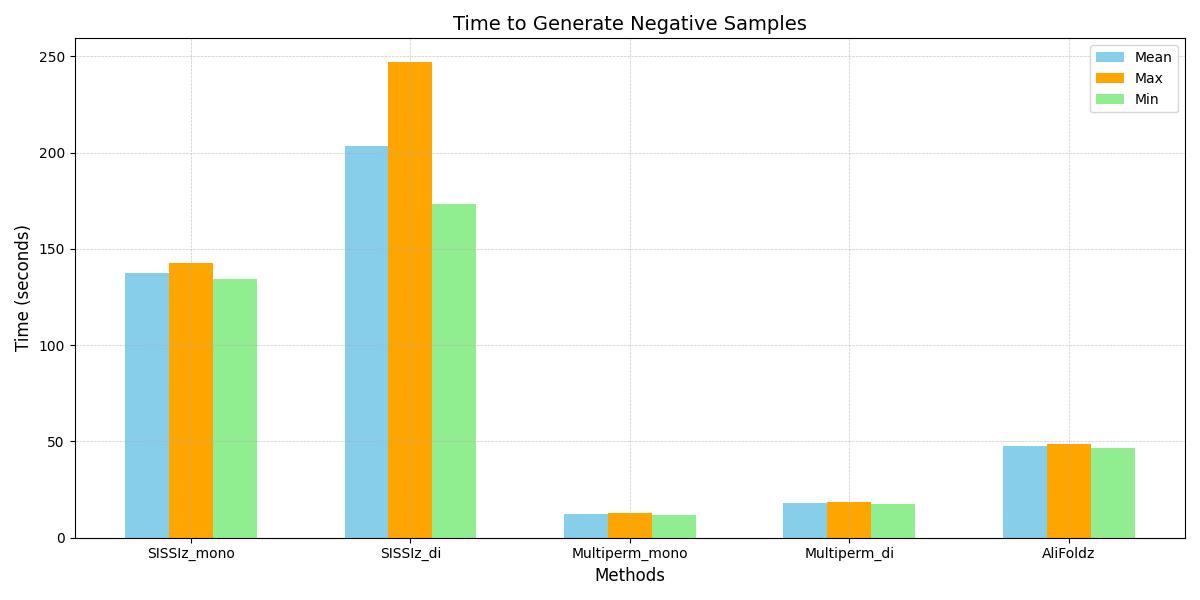
\includegraphics[scale=0.5]{Randomisation/Bar Chart.png}
    \caption{Display of the maximum, average and minimum time per 1000 samples}
    \label{fig:bar_chart}
\end{figure}


The SISSIz method requires significantly more time to simulate the randomized alignments. SISSIz mono requires an average of around 140 seconds per 1000 files, while SISSIz di is significantly slower at over 200 seconds. In contrast, the shuffle methods are 5 to 10 times faster, with Multiperm mono being the fastest method at only around 15 seconds per 1000 files.


\begin{figure}[H]
    \centering
    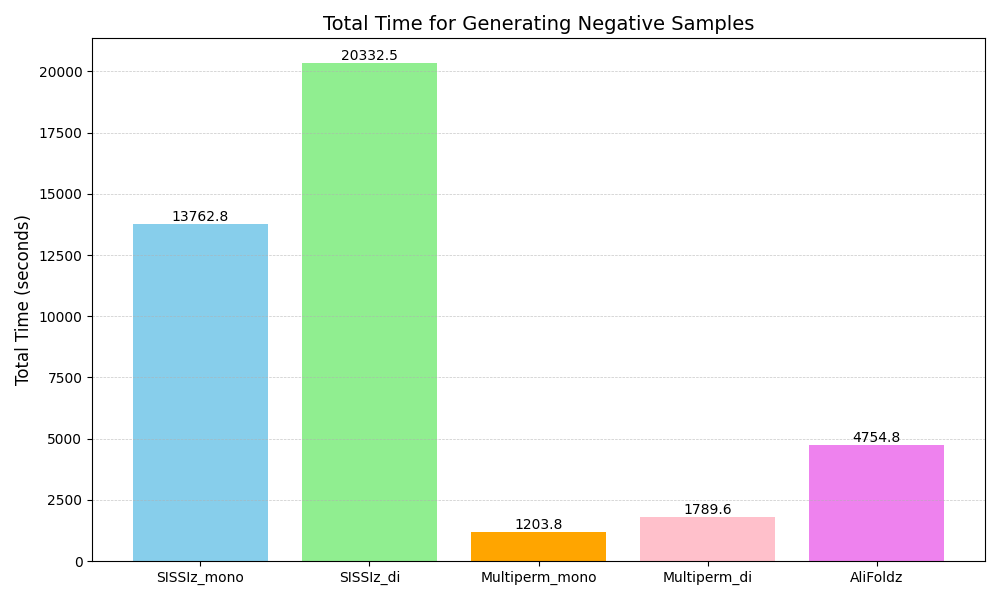
\includegraphics[scale=0.5]{Randomisation/Bar Chart Total Times.png}
    \caption{Gesamtzeiten für jedes Werkzeug}
    \label{fig:bar_chart_total}
\end{figure}


In terms of the total time for the simulation and shuffling of 100,000 alignments, SISSIz requires the most time. The di variant takes 20,332.5 seconds, while the mono variant is slightly faster at 13,762.8 seconds. The shuffle methods, on the other hand, require less than 5,000 seconds.


\begin{figure}[H]
    \centering
    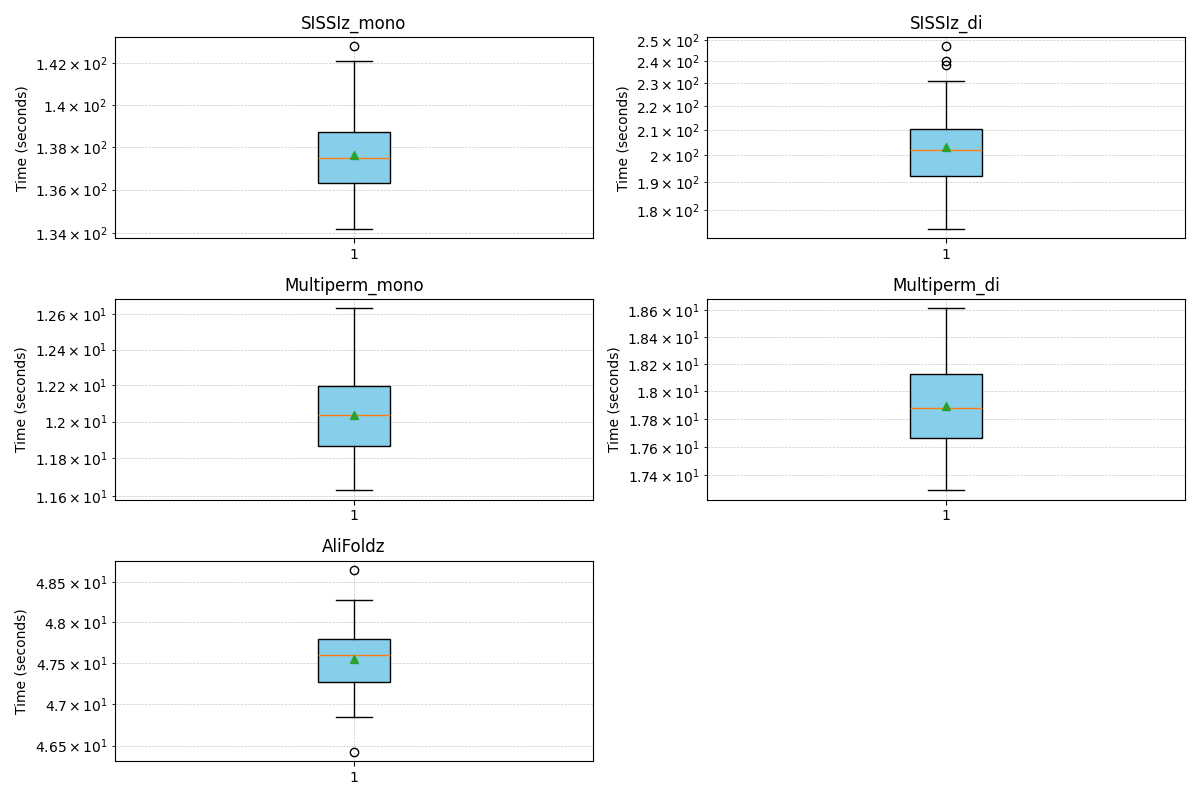
\includegraphics[scale=0.5]{Randomisation/Boxplot.png}
    \caption{Boxplot of the runtimes of the methods}
    \label{fig:boxplot_randomisation}
\end{figure}

\clearpage

\section{RNAz Data analysis}

Started the pipeline again to time how long RNAz takes to predict and then compare it to SISSIz and the other AI tools.


This section presents the results of the RNAz data analysis.



\begin{figure}[H]
    \centering
    \includegraphics[scale=0.5]{RNAz_prediction/Boxplot Consensus MFE.png}
    \caption{Consens Minimum Free Energy (MFE)}
    \label{fig:boxplot_mfe}
\end{figure}


The boxplot for the consensus MFE shows that the two SISSIz methods are above the threshold value of -20 kcal/mol, which indicates that the RNA structure was almost completely destroyed. In contrast, the shuffle methods show values below -20 kcal/mol. Alifoldz hardly managed to destroy the RNA structure, apart from a few alignments.


\begin{figure}[H]
    \centering
    \includegraphics[scale=0.5]{RNAz_prediction/Boxplot Structure conservatlion index.png}
    \caption{Structure preservation index (SCI)}
    \label{fig:boxplot_sci}
\end{figure}


The boxplot for the structure conservation index (SCI) also shows that all methods affected the RNA structure, with SISSIz achieving the best results. Alifoldz performed the worst here and was almost unable to destroy the structure in some alignments.


\begin{figure}[H]
    \centering
    \includegraphics[scale=0.5]{RNAz_prediction/Boxplot SVM RNA-class probability.png}
    \caption{SVM RNA-class probability}
    \label{fig:boxplot_svm}
\end{figure}


The SVM RNA class probability does not clearly indicate that the RNA structure has been destroyed, as all measurable values are well above the threshold value of 0.9. The lowest value is only 0.987, which indicates an intact RNA structure.

Additionally, I wanted to create a plot with the z-score, but the mean z-score provided by RNAz only describes the mean value of the mean single sequence MFE, which cannot be compared to the z-score provided by SISSIz

\clearpage

\section{SISSIz Data analysis}

This section presents the results of the SISSIz data analysis.


\begin{figure}[H]
    \centering
    \includegraphics[scale=0.5]{SISSIz_prediction/Consensus Minimum Free Energy (MFE).png}
    \caption{Consens Minimum Free Energy (MFE)}
    \label{fig:sissiz_mfe}
\end{figure}


The boxplot for the consensus MFE shows that the two SISSIz methods are above the threshold value of -20 kcal/mol, which indicates that the RNA structure was almost completely destroyed. In contrast, the shuffle methods show values below -20 kcal/mol. Alifoldz hardly managed to destroy the RNA structure, apart from a few alignments.


\begin{figure}[H]
    \centering
    \includegraphics[scale=0.5]{SISSIz_prediction/Structural Conservation Index (SCI).png}
    \caption{Structure preservation index (SCI)}
    \label{fig:sissiz_sci}
\end{figure}


The boxplot for the structure conservation index (SCI) shows that all methods affected the RNA structure, with SISSIz achieving the best results. Alifoldz performed the worst and was almost unable to destroy the alignments.


\begin{figure}[H]
    \centering
    \includegraphics[scale=0.5]{SISSIz_prediction/z-score.png}
    \caption{Z-Scores}
    \label{fig:sissiz_zscore}
\end{figure}


The z-scores confirm the previous results and show that SISSIz has almost completely destroyed the RNA structure. The threshold values are between -4 and +4, where by everything below -4 is considered an almost intact RNA structure. This is also evident from the positive alignments of SISSI.

\clearpage

\section{Tasks for KW5}

\begin{itemize}
    \item Calculation of the z-score of the RNA analysis in order to compare it with SISSIz
    \item Evaluation of the performance of RNAz and SISSIz
    \item Improve and adapt the pipeline diagram.
    \item Add the native alignments to the pipeline diagram.
    \item Consider which Ai tools I use for the evaluation of the alignments
\end{itemize}


\end{document}

Summary KW5 

\documentclass{article}
\usepackage{graphicx} % Required for inserting images
\usepackage{hyperref}
\usepackage{setspace}
\usepackage{listings}
\usepackage{float}
\usepackage[font=small,labelfont=bf]{caption}
\usepackage[a4paper, margin=1in]{geometry}
\usepackage{setspace}  
\onehalfspacing
\usepackage{hyperref}
\usepackage{xcolor}
\hypersetup{
    colorlinks=true, 
    linkcolor=blue, 
    urlcolor=blue,  
}

% Einstellungen für Code Listings
\lstset{
basicstyle=\ttfamily\small,
breaklines=true,
frame=single
}

\setlength{\parindent}{0pt}
\setlength{\textfloatsep}{0pt}

\title{KW5 Summary}
\author{Stefan Redl}
\begin{document}
\maketitle

\section{Pipeline}

\begin{large}
In the first run, RNA sequences from Bacillus subtilis with 78 sequences and 401 alignments were used and subsequently randomized with SISSI. Subsequently, for each positive sample generated, 1,000 negative samples were created using shuffle and simulation methods in order to destroy the RNA secondary structure as far as possible. This was done using the following methods:

\begin{itemize}
    \item MultiPerm v0.94 (mono- and dinucleotide conservation)
    \item aln-shuffle (mononucleotide conservation only)
    \item SISSIz v3.0 (mono- and dinucleotide conservation)
\end{itemize}

After the RNA secondary structure has been destroyed, it is checked whether it has been completely eliminated. I used the RNAz and SISSIz tools for this. The prediction is later extended with AI tools.

\begin{itemize}
    \item RNAz v2.1.1
    \item SISSIz v3.0
    \item SPOT-RNA2 \href{https://doi.org/10.1093/bioinformatics/btab165}{\textbf{[1]}} \href{https://github.com/jaswindersingh2/SPOT-RNA2}{\textbf{[2]}}
    \item DeepFoldRNA \href{https://doi.org/10.1101/2022.05.15.491755}{\textbf{[3]}} \href{https://github.com/robpearc/DeepFoldRNA}{\textbf{[4]}}
    \item RNA-MSM \href{https://doi.org/10.1093/nar/gkad1031}{\textbf{[5]}} \href{https://github.com/yikunpku/RNA-MSM}{\textbf{[6]}} 
\end{itemize}

The results were then visualized with Python, evaluated and compared with other methods.

After completion of the first run, an RNA sequence of Bacillus subtilis is extracted from the RFAM database. In this run, randomization with SISSI is omitted. Instead, the RNA secondary structure is destroyed directly and then analyzed with RNAz, SISSIz and the AI models.

\begin{figure}[H]
    \centering
    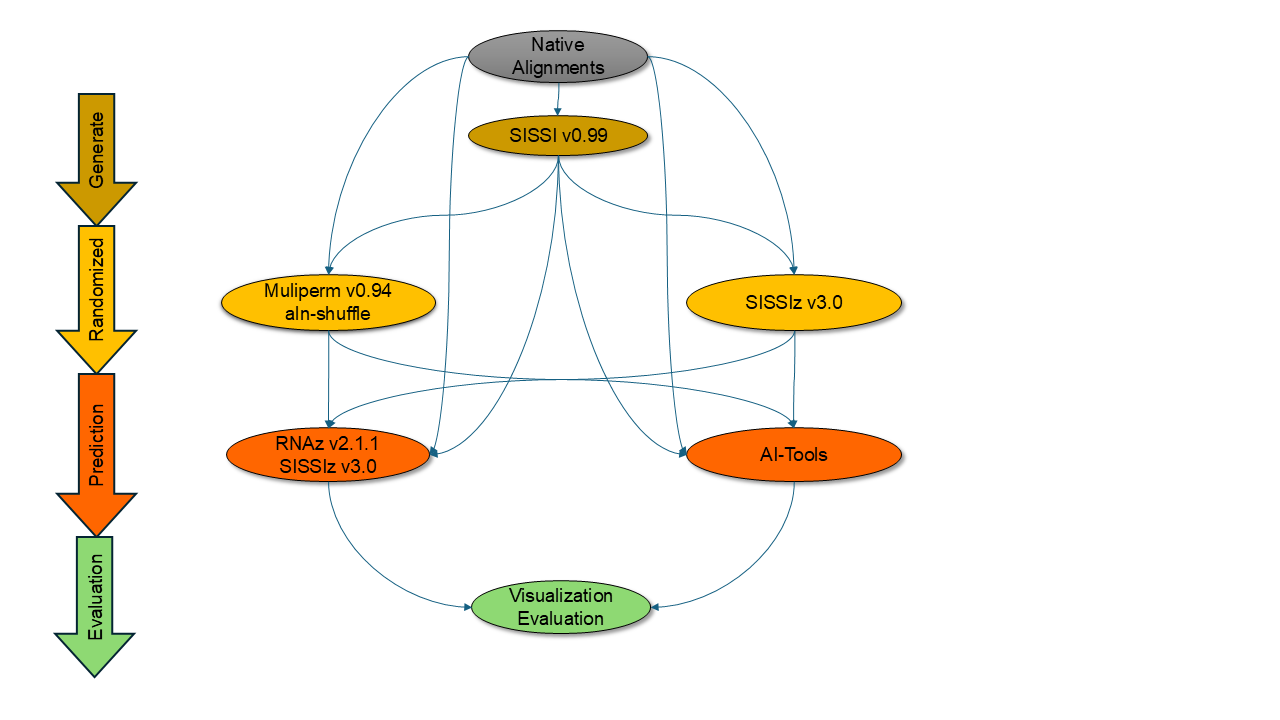
\includegraphics[scale=0.7]{Pipeline Diagramm.png}
    \caption{Pipeline}
    \label{fig:bar_chart}
\end{figure}

\section{Time capture from RNAz and SISSIz}

I have integrated a time measurement into the scripts RNAz-prediction.py and SISSIz-prediction.py. An intermediate measurement is carried out after every 1,000 predictions. This enables a more precise evaluation of the performance of the prediction tools used.

The test is carried out on a system with 24 cores to ensure a fair and comparable performance analysis.

\section{Research about the p-value and mean-z-score in RNAz}

I have noticed that the mean z-score is calculated differently in RNAz than in SISSIz. Therefore, I still need to check how I can adjust the calculation in RNAz to ensure direct comparability.

One possible solution would be to use RNAalifold. This could calculate the partial sequences from the Clustal files and then determine the mean value and the standard deviation.

\section{Copy Data all Data to my Sytem}

Because the FH get a new Server on Monday the 3th, i started to copy all necessary Folders into my System.

\section{Tasks for KW6}

\begin{itemize}
    \item Extract an RNA sequence from the RFAM database to start the second run without SISSI
    \item Select two suitable AI tools and understand their process 
    \item start a run from SISSI-prediction.py with the integrate time capturing
    \item as soon as the new fh server arrives, I will have to reinstall all the tools and recreate my setup
\end{itemize}


\section{References SPOT-RNA2}

\begin{itemize}
    \item[\textbf{[1]}] \url{https://doi.org/10.1093/bioinformatics/btab165} \par
    \item[\textbf{[2]}] \url{https://github.com/jaswindersingh2/SPOT-RNA2}
\end{itemize}


\section{References DeepFoldRNA}

\begin{itemize}
    \item[\textbf{[3]}] \url{https://doi.org/10.1101/2022.05.15.491755} \par
    \item[\textbf{[4]}] \url{https://github.com/robpearc/DeepFoldRNA}
\end{itemize}

\section{References RNA-MSM}

\begin{itemize}
    \item[\textbf{[5]}] \url{https://doi.org/10.1093/nar/gkad1031} \par
    \item[\textbf{[6]}] \url{https://github.com/yikunpku/RNA-MSM}
\end{itemize}

\end{large}
\end{document}


Summary KW6 and KW7

\documentclass{article}
\usepackage{graphicx} % Required for inserting images
\usepackage{hyperref}
\usepackage{setspace}
\usepackage{listings}
\usepackage{float}
\usepackage[font=small,labelfont=bf]{caption}
\usepackage[a4paper, margin=1in]{geometry}
\usepackage{setspace}  
\onehalfspacing
\usepackage{hyperref}
\usepackage{xcolor}
\hypersetup{
    colorlinks=true, 
    linkcolor=blue, 
    urlcolor=blue,  
}

% Einstellungen für Code Listings
\lstset{
basicstyle=\ttfamily\small,
breaklines=true,
frame=single
}

\setlength{\parindent}{0pt}
\setlength{\textfloatsep}{0pt}

\title{KW6 and KW7 Summary}
\author{Stefan Redl}
\begin{document}
\maketitle

\begin{large}

\section{Pipeline}

\section{Evaluate the timing of RNAz}

Started to evaluate the timing from RNAz during the prediction. 
To compare it with SISSIz i started also a timing, but i must stop it, because the FH get a new Server. To be continued.

\section{Searching for b.subtilis}

I started to research for nativ b.subtilis alignments in the RFAM Database, but i cannot find the right alignments. After the Meeting with Tanja i restarted my research and try to translate the B.subtilis.ct2 file from SISSI into a fasta file. 
I entered the Fasta Sequenze into the RFAM database and got 4 identical hits. To be continued

\clearpage

\section{SPOT-RNA2\href{https://doi.org/10.1093/bioinformatics/btab165}{\textbf{[1]}}}

\textbf{Title:}\par
Improved RNA Secondary Structure and Tertiary Base Pairing Prediction Using Evolutionary Profiles, Mutational Coupling, and 2D Transfer Learning \\[0.5em]

\textbf{Authors:} \par 
Jaswinder Singh, Kuldip Paliwal, Tongchuan Zhang, Jaspreet Singh, Thomas Litfin, Yaoqi Zhou \\[0.5em]

\textbf{Introduction:}\par

The discovery of numerous non-coding RNAs, especially long non-coding RNAs, has revolutionized our understanding of their biological functions.
The ability to accurately determine their secondary and tertiary structures is limited by the constraints of experimental techniques.
Computational prediction methods have significantly improved in recent years with deep learning and transfer learning.\\[0.5em]

\textbf{Motivation:}\par

Accurate RNA structure prediction is crucial for understanding its function.
Traditional experimental methods such as X-ray crystallography and NMR are expensive and time-consuming, necessitating efficient computational methods.\\[0.5em]

\textbf{Methods:}\par

The proposed method, SPOT-RNA2, extends previous approaches by incorporating evolutionary profiles and mutational coupling.
Input data includes:
    \begin{itemize}
        \item One-hot encoding of the RNA sequence.
        \item Predicted base-pair probabilities from the single-sequence method LinearPartition.
        \item Position-Specific Scoring Matrix (PSSM) and two-dimensional Direct Coupling Analysis (DCA) information.
        \item The method employs an ensemble of deep neural networks, optimized from SPOT-RNA to improve prediction accuracy. \\[0.5em]
    \end{itemize} 

\textbf{Results:}\par

SPOT-RNA2 demonstrates significant improvements in predicting canonical and non-canonical base pairs as well as tertiary interactions like pseudoknots.
The method achieves an F1-score above 0.8 for 14 out of 16 tested RNAs with more than 1000 homologous sequences.
The integration of artificial homologous sequences generated through deep mutational scanning further improves accuracy. \\[0.5em]

\textbf{Availability and Implementation:}\par

SPOT-RNA2 is available as standalone software and via a web server.
The datasets used can be downloaded from GitHub and the web server.\\[0.5em]

\textbf{Performance Evaluation:}\par

Performance is assessed using F1-score and Matthews correlation coefficient (MCC).
SPOT-RNA2 outperforms existing RNA secondary structure prediction methods in various test scenarios, including pseudoknot and non-canonical base pair prediction.\\[0.5em]

\textbf{Comparison with Existing Methods:}\par

SPOT-RNA2 is compared with other single-sequence and alignment-based prediction methods.
Results show consistently higher accuracy, particularly for RNAs with complex base-pairing patterns.\\[0.5em]

\textbf{Conclusion:}\par

SPOT-RNA2 is a powerful tool for RNA structure prediction, demonstrating the potential of evolutionary information to enhance prediction accuracy.
The method is particularly beneficial for RNAs with a large number of homologous sequences, improving prediction accuracy.\\[0.5em]

\textbf{Future Perspectives:}\par

Combining natural and artificial homologous sequences could further improve prediction accuracy.
The development of more efficient algorithms for handling longer RNA sequences and reducing computational time is a future goal.\\[0.5em]

\textbf{Contact Information:}\par

Jaswinder Singh: jaswinder.singh3@griffithuni.edu.au
Yaoqi Zhou: yaoqi.zhou@griffith.edu.au\\[0.5em]

\clearpage

\section{DeepFoldRNA\href{https://doi.org/10.1101/2022.05.15.491755}{\textbf{[2]}}}

\textbf{Title:}\par
De Novo RNA Tertiary Structure Prediction at Atomic Resolution Using Geometric Potentials from Deep Learning\\[0.5em]

\textbf{Authors:}\par
Robin Pearce, Gilbert S. Omenn, Yang Zhang\\[0.5em]

\textbf{Introduction:}\par

RNA molecules play a crucial role in many biological processes, with their functions strongly dependent on their three-dimensional structures.
There is a significant gap between the number of known RNA sequences and experimentally determined RNA structures.
Effective computational methods for RNA structure prediction are urgently needed, particularly for non-coding RNAs.\\[0.5em]

\textbf{DeepFoldRNA:}\par

DeepFoldRNA is a novel method combining deep self-attention neural networks and gradient-based folding simulations.
The approach aims to determine the spatial position of each atom in an RNA molecule solely from its nucleotide sequence.\\[0.5em]

\textbf{Methods:}\par

\textbf{Restraint Generation Module:}
    Multiple sequence alignments (MSAs) are created through iterative searches in RNA databases.
    Self-attention neural networks predict spatial constraints (restraints) such as pairwise distances and backbone torsion angles.\\[0.5em]
\textbf{Structure Construction Module:}
    Predicted geometric restraints are converted into composite potentials guiding L-BFGS folding simulations.
    These simulations enable rapid and precise RNA folding.\\[0.5em]

\textbf{Results:}\par

DeepFoldRNA was tested on two independent benchmark datasets: one from Rfam families and one from RNA-Puzzles
The method achieved an average RMSD of 2.68 Å and a TM-score of 0.757, significantly improving over existing methods.
DeepFoldRNA folds medium-sized RNAs in about one minute on average, 350-4000 times faster than leading Monte Carlo simulation approaches.\\[0.5em]

\textbf{Applications:}\par

Its high speed and accuracy allow large-scale applications in atomic RNA structure modeling.
The method could be extended to RNA-protein interactions and RNA complexes to better understand molecular and cellular functions.\\[0.5em]

\clearpage

\section{RNA-MSM\href{https://doi.org/10.1093/nar/gkad1031}{\textbf{[3]}}}

\textbf{Title:}\par
Multiple Sequence Alignment-based RNA Language Model and Its Application to Structural Inference\\[0.5em]

\textbf{Authors:}\par
Yikun Zhang, Mei Lang, Jiuhong Jiang, et al.\\[0.5em]

\textbf{Introduction:}\par

RNA and DNA are harder to interpret than proteins, as they have only four letters compared to twenty for proteins.
Previous RNA language models based on BERT-like architectures fail to capture evolutionary information effectively.
An unsupervised RNA language model based on multiple sequence alignments (MSA) could improve RNA structure and function prediction.\\[0.5em]

\textbf{RNA-MSM:}\par

RNA-MSM was developed to utilize homologous RNA sequences from RNAcmap, generating more homologs than manually curated databases like Rfam.
The model uses an unsupervised learning architecture producing two-dimensional attention maps and one-dimensional embeddings encoding structural information.\\[0.5em]

\textbf{Results:}\par

RNA-MSM’s generated attention maps and embeddings accurately predict 2D base-pairing probabilities and 1D solvent accessibilities.
The model outperforms techniques like SPOT-RNA2 and RNAsnap2 in base pair and solvent accessibility predictions.
The study emphasizes challenges in RNA structure prediction compared to proteins and highlights the importance of evolutionary information.\\[0.5em]

\textbf{Availability:}\par

Source codes, models, and datasets are publicly available on Zenodo.\\[0.5em]

\clearpage

\section{Sean Eddy and Elena Rivas\href{https://www.mcb.harvard.edu/department/news/mcb-welcomes-sean-eddy-and-elena-rivas/}{\textbf{[4]}}}

Sean Eddy and Elena Rivas, renowned computational biologists from the Janelia Research Campus, are joining the Department of Molecular and Cellular Biology (MCB) this fall. Eddy will serve as a professor, while Rivas will take on the role of senior research fellow and lecturer. Their work focuses on the significance of RNA in evolution, utilizing advanced computational tools to analyze RNA sequences' structure, function, and evolutionary history.\\[0.5em]

Eddy's journey into science began in rural Pennsylvania, inspired by his mother, who pursued biology while raising six children. He initially studied physics at Caltech but switched to biology, eventually earning a PhD in molecular biology at the University of Colorado. His research on self-splicing RNA and the movement of introns led him to develop algorithms for RNA analysis, culminating in the creation of HMMER and Infernal software.\\[0.5em]

Rivas, originally a particle physicist, transitioned to biology after realizing her passion for problem-solving in a more rewarding field. She joined Eddy's lab, where she applied her physics background to RNA research, developing programs to identify RNA genes and their evolutionary significance.\\[0.5em]

At Janelia, both Eddy and Rivas made significant contributions to RNA research and software development. Eddy focused on enhancing Infernal and exploring cell-type specific genomics, while Rivas worked on probabilistic models for genome sequence interpretation.\\[0.5em]

Now at MCB, they are excited to build a new lab, collaborate with diverse researchers, and tackle new scientific challenges. Eddy, who has a history with MCB, feels a strong connection to the department, viewing it as a second home. Together, they look forward to refining their current projects and exploring new avenues in RNA research and beyond.\\[0.5em]

\clearpage

\section{Evolutionary conservation of RNA sequence and structure\href{https://pubmed.ncbi.nlm.nih.gov/33754485/}{\textbf{[5]}}}

The article by Elena Rivas titled "Evolutionary conservation of RNA sequence and structure" provides a comprehensive analysis of the role of RNA in biological processes and the challenges associated with predicting its structural properties. In recent decades, scientific interest has increasingly shifted from DNA to RNA, driven by the recognition that RNA serves not only as an intermediary molecule in protein synthesis but also plays a crucial role in various regulatory and structural functions within the cell. In particular, non-coding RNAs, including long non-coding RNAs (lncRNAs), have been identified as essential for gene regulation and the maintenance of cellular homeostasis.\\[0.5em]

\textbf{Importance of RNA Structure}\par
Rivas argues that predicting RNA structure from a single sequence is insufficient to establish the functional relevance of that structure. Many random RNA sequences can exhibit complex and plausible structures that are indistinguishable from those of functional RNAs. Therefore, it is critical to analyze the evolutionary signatures left by conserved RNAs to determine whether an RNA possesses a functionally relevant structure. The article emphasizes that identifying conserved RNA structures is not only vital for understanding RNA function but also for reconstructing the evolutionary history of organisms.\\[0.5em]

\textbf{Methods for Analyzing RNA Conservation}\par
The article describes various statistical approaches for measuring the conservation of RNA structures, particularly the application of covariation analyses. These methods allow for the differentiation between structural RNA conservation and covariation arising from independent phylogenetic substitutions. Rivas highlights the necessity of identifying false positives that may arise from artifacts, such as the inclusion of pseudogenes in alignments, as these can significantly compromise the analysis of RNA structure conservation.\\[0.5em]

\textbf{Covariation and Variability}\par
A central theme of the article is the analysis of sequence variations and their patterns to support or refute the existence of a conserved RNA structure. Rivas explains that a conserved RNA sequence does not necessarily imply a conserved structure. Instead, supporting evidence for a conserved structure requires a specific pattern of variations indicative of evolutionary preservation. The article underscores that there are also variation patterns that support the absence of a conserved structure, illustrating the complexity of RNA evolution.\\[0.5em]

\textbf{Challenges in Identifying Conserved RNA Structures}\par
Rivas discusses the challenges associated with identifying new evolutionarily conserved RNA structures. She emphasizes that the integration of sequence and structural information, along with the consideration of covariation and variability, is crucial for understanding the evolutionary significance of RNA. The article concludes by stating that developing methods for analyzing RNA structure and function, which incorporate both evolutionary and structural information, is of paramount importance for elucidating the mechanisms of RNA function and evolution.\\[0.5em]

\textbf{Conclusion}\par
Overall, Rivas's article offers profound insights into the current challenges and advancements in RNA research, particularly regarding the identification and analysis of conserved RNA structures. The findings from this research could not only deepen the understanding of the biological functions of RNA but also pave the way for new approaches to investigate the evolution of RNA molecules and their roles in cellular regulation and function.\\[0.5em]

\clearpage

\section{sincFold\href{https://pubmed.ncbi.nlm.nih.gov/38855913/}{\textbf{[6]}}\href{https://github.com/sinc-lab/sincFold}{\textbf{[7]}}}

The article presents "sincFold," a novel end-to-end deep learning model designed for predicting RNA secondary structures by learning both short- and long-range interactions from RNA sequences. This research addresses the longstanding challenge of accurately predicting RNA secondary structures, which are crucial for understanding the functional roles of RNA molecules in biological processes.\\[0.5em]

\textbf{Motivation and Background}\par

RNA molecules, including both coding and non-coding RNAs, play vital roles in various biological functions. The ability to predict their secondary structures from sequences is essential for elucidating their functions and evolutionary significance. Traditional methods for RNA secondary structure prediction have relied on thermodynamic models and dynamic programming, which have limitations in performance. Recent advancements in deep learning have shown promise in improving prediction accuracy, yet there remains significant room for enhancement.\\[0.5em]

\textbf{Methodology}\par

sincFold employs a two-stage deep learning architecture that integrates both one-dimensional (1D) and two-dimensional (2D) residual neural networks. The model takes a one-hot encoded RNA sequence as input and predicts a contact matrix that represents nucleotide interactions. The first stage focuses on learning local patterns in the 1D representation of the sequence, while the second stage captures distant relationships through a 2D representation.\\[0.5em]

\textbf{Key components of the sincFold architecture include}\par

\begin{itemize}
    \item \textbf{1D Residual Networks} 
    These networks facilitate the learning of short-range interactions by stacking identity blocks that help propagate signals and mitigate vanishing gradient issues.
    \item \textbf{2D Residual Networks} 
    After obtaining a 1D encoding, the model transitions to a 2D representation to learn long-range interactions, enhancing the model's ability to predict complex RNA structures.\\[0.5em]
\end{itemize}

\textbf{Results}\par

Extensive experiments were conducted using several benchmark datasets, including RNAstralign and ArchiveII, to evaluate the performance of sincFold. The model demonstrated superior accuracy in predicting RNA secondary structures compared to classical methods and other state-of-the-art deep learning approaches. The results indicate that sincFold can effectively learn the intricate patterns of RNA interactions with minimal physical assumptions.\\[0.5em]

\textbf{Performance Metrics}\par

The performance of sincFold was assessed using metrics such as the F1 score, which evaluates the accuracy of predicted base pairs against reference structures. The model achieved high F1 scores, particularly excelling in the prediction of both canonical and non-canonical base pairs.\\[0.5em]

\textbf{Conclusion}\par

sincFold represents a significant advancement in RNA secondary structure prediction, leveraging deep learning techniques to capture both short- and long-range interactions effectively. The model's end-to-end learning approach allows for accurate predictions without the need for multiple sequence alignments or extensive pre-processing. The authors have made the source code publicly available, facilitating further research and development in the field of RNA bioinformatics.\\[0.5em]

\clearpage

\section{Tasks for KW8}

\begin{itemize}
    \item Revise the presentation
    \item Ask Frau Graf if she has already created a user for me so that I can run through my pipeline again.
    \item Reconfigure the server for my pipeline
    \item Research about native bacillus subtilis alignments
    \item Start with the Master's thesis (introduction, methods used, ...
    \item Read following Papers and make a summary
    \begin{itemize}
        \item https://pubmed.ncbi.nlm.nih.gov/33845850/
        \item https://pubmed.ncbi.nlm.nih.gov/36596869/
        \item https://pubmed.ncbi.nlm.nih.gov/39526405/
        \item https://pubmed.ncbi.nlm.nih.gov/39526405/
    \end{itemize}
\end{itemize}

\section{References}

\begin{itemize}
    \item[\textbf{[1]}] \url{https://doi.org/10.1093/bioinformatics/btab165} \par
    \item[\textbf{[2]}] \url{https://doi.org/10.1101/2022.05.15.491755}
    \item[\textbf{[3]}] \url{https://doi.org/10.1093/nar/gkad1031} \par
    \item[\textbf{[4]}] \url{https://www.mcb.harvard.edu/department/news/mcb-welcomes-sean-eddy-and-elena-rivas/}
    \item[\textbf{[5]}] \url{https://pubmed.ncbi.nlm.nih.gov/33754485/} \par
    \item[\textbf{[6]}] \url{https://pubmed.ncbi.nlm.nih.gov/38855913/} \par
    \item[\textbf{[7]}] \url{https://github.com/sinc-lab/sincFold} \par
\end{itemize}


\end{large}
\end{document}

Summary KW8 and KW9

\documentclass{article}
\usepackage{graphicx} % Required for inserting images
\usepackage{hyperref}
\usepackage{setspace}
\usepackage{listings}
\usepackage{float}
\usepackage[font=small,labelfont=bf]{caption}
\usepackage[a4paper, margin=1in]{geometry}
\usepackage{setspace}  
\onehalfspacing
\usepackage{hyperref}
\usepackage{xcolor}
\hypersetup{
    colorlinks=true, 
    linkcolor=blue, 
    urlcolor=blue,  
}

% Einstellungen für Code Listings
\lstset{
basicstyle=\ttfamily\small,
breaklines=true,
frame=single
}

\setlength{\parindent}{0pt}
\setlength{\textfloatsep}{0pt}

\title{KW8 and KW9 Summary}
\author{Stefan Redl}
\begin{document}
\maketitle

\begin{large}

\section{Installation of the required software on the new server}

All tools previously used on the old server were reinstalled and their functionality checked. In addition, the installation was adapted so that the programs are accessible user-wide and can be executed from any directory.

\section{Adaptation of the presentation}

The updated pipeline was added to the presentation. In addition, the results of the time measurements for the various tools used to generate the negative samples were integrated.

\section{Performance measurement of the SISSIz predictions }

After successfully setting up the server, a new run with SISSIz was carried out. A time stamp was recorded at regular intervals (after every 1,000 predictions) and written to a log file. In addition, the number of CPU cores used was increased from 24 to 64, reducing the expected runtime to an average of 10 days.

\section{Native Alignments from B.subtilis}

A search of the RFAM database for alignments of Bacillus subtilis identified 62 sequences, each comprising between 370 and 401 base pairs. The central question is whether these sequences can be used as a reference for a comparison with the alignments randomized by SISSI.

\clearpage

\section{Comparative genomics identifies thousands of candidate structured RNAs in human microbiomes\href{https://pubmed.ncbi.nlm.nih.gov/33845850/}{\textbf{[1]}}}

\textbf{Industruction:}\par
In their study “Comparative genomics identifies thousands of candidate structured RNAs in human microbiomes”, Brayon J. Fremin and Ami S. Bhatt investigated the presence and diversity of structured RNAs within the human microbiome. Structured RNAs perform diverse bioregulatory functions in microbes. Although hundreds of such RNAs have been predicted using informative approaches, much of the metagenomic data of the human microbiome remained unexplored due to computational limitations.\\[0.5em]

\textbf{Methods:}\par
The authors developed a pipeline to identify potential structured RNAs. First, genes in the Human Microbiome Project 2 (HMP2) were annotated with Prodigal. They then identified homologous intergenic regions using HS-BLASTN. Conserved regions were grouped and scored using RNAphylo, R-scape and RNAcode. Known RNAs from the Rfam database were excluded, and remaining candidates were matched against HMP2 using cmsearch to ensure unique hits. Finally, these regions were matched against the nr database using BLASTx to ensure that they were not protein coding.\\[0.5em]

\textbf{Results:}\par
Using this approach, the researchers identified 3,161 potential structured RNAs and 2,022 additional candidates with overlaps to the nr database. A large number of these RNAs, including tmRNAs, antitoxins and ribosomal protein leaders, were found in different taxa. Genomic neighborhood analysis revealed frequent associations with specific protein domains, indicating possible regulatory functions.\\[0.5em]

\textbf{Conclusions:}\par
The developed pipeline enables conservative predictions of thousands of new potential structured RNAs in the human microbiome. These discoveries expand our understanding of RNA-based regulation in microbial communities and provide insights into the complex bioregulatory networks of the human microbiome.\\[0.5em]

\clearpage

\section{Long non-coding RNAs: definitions, functions, challenges and recommendations\href{https://pubmed.ncbi.nlm.nih.gov/36596869/}{\textbf{[2]}}}

\textbf{Industruction:}\par
In the review article “Long non-coding RNAs: definitions, functions, challenges and recommendations”, the authors shed light on the diverse aspects of long non-coding RNAs (lncRNAs). These RNAs, which are over 200 nucleotides long and are not translated into proteins, make up a significant proportion of the genomes of complex organisms\\[0.5em]

\textbf{Definition and classification:}\par
The term 'lncRNAs' encompasses a variety of transcripts, including those transcribed by RNA polymerase I, II, and III, as well as RNAs derived from processed introns. The variety of functions, isoforms and overlap with other genes complicates the classification and annotation of lncRNAs.\\[0.5em]

\textbf{Functions of lncRNAs:}\par
lncRNAs play a critical role in regulating many aspects of cell differentiation, development, and other physiological processes. Many lncRNAs bind to chromatin-modifying complexes, are transcribed by enhancers and promote the formation of nuclear condensates, indicating a close link between lncRNA expression and the spatial control of gene expression during development.\\[0.5em]

\textbf{Challenges in research:}\par
The rapid evolution of lncRNAs compared to protein-coding sequences, their cell-specific expression and the diversity of their functions pose considerable challenges for researchers. The identification of interaction partners and the determination of the specific functions of individual lncRNAs require comprehensive studies.\\[0.5em]

\textbf{Recommendations for future research:}\par
The authors emphasize the need for standardized methods for annotation and functional characterization of lncRNAs. They recommend the development of new technologies and approaches to better understand the complex roles of lncRNAs in cell biology and disease.\\[0.5em]

\clearpage

\section{RFAM 15: RNA families database in 2025\href{https://pubmed.ncbi.nlm.nih.gov/39526405/}{\textbf{[3]}}}

\section{Introduction}\par
The Rfam database is a comprehensive collection of RNA families represented by multiple sequence alignments, consensus secondary structures and covariance models. With the release of version 15.0 in September 2024, several significant updates have been made.\\[0.5em]

\textbf{Expansion of Rfamseq:}\par
The number of genomes in the Rfamseq database was increased from 14,772 in version 14.0 to 26,106 in version 15.0, an increase of 76 percent. This expansion aims to better reflect the genomes currently available.\\[0.5em]

\textbf{Integration of 3D structures:}\par
 In version 15.0, 25 additional RNA families have been reviewed and annotated with 3D information, bringing the total number of families containing such structural data to 65. This integration improves the accuracy of consensus secondary structures and annotations.\\[0.5em]

\textbf{Provision of a public MySQL database:}\par
Rfam now provides a publicly accessible, read-only MySQL database that is updated with each new version. This facilitates access to the latest data for the research community.\\[0.5em]

\section{Tasks for KW10}
\begin{itemize}
    \item Make the changes to the presentation discussed in the meeting with Tanja
    \item Compare Time Prediction from RNAz and SISSIz
    \item Research about native bacillus subtilis alignments
    \item Start with the Master's thesis (introduction, methods used, ...
\end{itemize}

\section{References}
\begin{itemize}
    \item[\textbf{[1]}] \url{https://pubmed.ncbi.nlm.nih.gov/33845850/} \par
    \item[\textbf{[2]}] \url{https://pubmed.ncbi.nlm.nih.gov/36596869/} \par
    \item[\textbf{[3]}] \url{https://pubmed.ncbi.nlm.nih.gov/39526405/} \par
\end{itemize}

\end{large}
\end{document}


Summary KW13 - KW16

\documentclass{article}
\usepackage{graphicx} % Required for inserting images
\usepackage{hyperref}
\usepackage{setspace}
\usepackage{listings}
\usepackage{float}
\usepackage[font=small,labelfont=bf]{caption}
\usepackage[a4paper, margin=1in]{geometry}
\usepackage{setspace}  
\onehalfspacing
\usepackage{hyperref}
\usepackage{xcolor}
\hypersetup{
    colorlinks=true, 
    linkcolor=blue, 
    urlcolor=blue,  
}

\usepackage{listings}
\usepackage{xcolor}

\lstset{
    language=Python,
    basicstyle=\ttfamily\small,
    keywordstyle=\bfseries\color{blue},
    commentstyle=\itshape\color{gray},
    stringstyle=\color{orange},
    showstringspaces=false,
    numbers=left,
    numberstyle=\tiny,
    breaklines=true,
    frame=single
    aboveskip=1em,
    belowskip=1em
}


% Einstellungen für Code Listings
\lstset{
basicstyle=\ttfamily\small,
breaklines=true,
frame=single
}

\setlength{\parindent}{0pt}
\setlength{\textfloatsep}{0pt}

\title{KW13 - KW16 Summary}
\author{Stefan Redl}
\begin{document}
\maketitle

\begin{large}

\section{Introduction to the ROC Curve Code}

A function is defined here that compares two data sets (positive and negative), adds artificial noise and then evaluates them using a random forest classifier. Parameters such as noise scale (strength of the noise) or labels can also be adjusted.

\begin{lstlisting}
def evaluate_classifier_with_noise(df_positive, df_negative, noise_scale=10, pos_label=1, neg_label=0, title_suffix=""):
\end{lstlisting}\par
\vspace{1em}

The most important libraries for data analysis, visualization and machine learning are imported.
\begin{lstlisting}
    # import the necessary libaries
    import numpy as np
    import pandas as pd
    import matplotlib.pyplot as plt
    import seaborn as sns
    from sklearn.ensemble import RandomForestClassifier
    from sklearn.model_selection import cross_val_predict
    from sklearn.metrics import confusion_matrix, classification_report, roc_curve, auc
\end{lstlisting}\par
\vspace{1em}

The transferred data records are copied (so as not to change the original data). They are then given a label (1 for positive, 0 for negative), which is required later for training the classifier.
\begin{lstlisting}
    # Set the labels 
    df_positive = df_positive.copy()
    df_negative = df_negative.copy()
    df_positive['Label'] = pos_label
    df_negative['Label'] = neg_label
\end{lstlisting}\par
\vspace{1em}

Here, additional noise is added to each data set. This results in a deliberate overlap of the positive and negative data points. Without this overlap, the classification task would be too trivial and not realistic. This makes the classification more realistic and more challenging for the model (random forest).
\begin{lstlisting}
    # Add noise to the 
    df_positive['z-score calculated from 7. 8. and 9.'] += np.random.normal(loc=0, scale=noise_scale, size=len(df_positive))
    df_negative['z-score calculated from 7. 8. and 9.'] += np.random.normal(loc=0, scale=noise_scale, size=len(df_negative))
\end{lstlisting}\par
\vspace{1em}

The two data sets are merged into a common DataFrame, which simplifies subsequent processing (training and visualization).
\begin{lstlisting}
    # Combine the datasets 
    data = pd.concat([df_positive, df_negative], ignore_index=True)
\end{lstlisting}\par
\vspace{1em}

The comparison between the two datasets is visualized to illustrate the distribution of true positives (TP), true negatives (TN), false positives (FP), and false negatives (FN).

\begin{lstlisting}
    # Visualize the Comparison between the two Datasets to illustrate the TN, FN, TP and FP
    sns.histplot(data=data, x='z-score calculated from 7. 8. and 9.', hue='Label', kde=True, bins=50)
    plt.title(f"Distribution of z-scores with noise {title_suffix}")
    plt.xlabel("z-Score")
    plt.ylabel("Anzahl")
    plt.show()
\end{lstlisting}\par
\vspace{1em}
The feature matrix X and the target variable y are prepared. A random forest classifier with 100 decision trees is then created. random_state=42 ensures reproducibility.

\begin{lstlisting}
    # Preparation for the Randomforest Classifier
    X = data[['z-score calculated from 7. 8. and 9.']]
    y = data['Label']
    model = RandomForestClassifier(n_estimators=100, random_state=42)
\end{lstlisting}\par
\vspace{1em}
The model is evaluated with 5-fold cross-validation to avoid overfitting. Both the predicted classes (y_pred) and the probabilities for the positive class (y_proba) are calculated.

\begin{lstlisting}
    # Crossvalidation is added to avoid overfitting
    y_pred = cross_val_predict(model, X, y, cv=5, method='predict')
    y_proba = cross_val_predict(model, X, y, cv=5, method='predict_proba')[:, 1]
\end{lstlisting}\par
\vspace{1em}
The confusion matrix shows the number of correctly and incorrectly classified cases. 


\begin{itemize}
        \item True Negative = RNA structure was destroyed and correctly predicted
        \item True Positive = RNA structure was not destroyed and correctly predicted
        \item False Negative = RNA structure was not destroyed but not correctly predicted
        \item False Positive = The RNA structure was destroyed, but the model incorrectly predicted it as intact (false positive) \\[0.5em]
\end{itemize} 

The classification report provides key figures such as Precision, Recall, F1-Score and Accuracy - these are important metrics for evaluating the classifier.
\begin{lstlisting}
    # Evaluating of the Confusion Matrix and the Classificaltion
    print(" Confusion Matrix:\n", confusion_matrix(y, y_pred))
    print("\n Classification Report:\n", classification_report(y, y_pred))
\end{lstlisting}\par
\vspace{1em}

The ROC curve compares the true positive rate against the false positive rate for different threshold values. The AUC value (Area Under Curve) measures the quality of the separation between the classes.
\begin{lstlisting}
    # Calculation of the AUC 
    fpr, tpr, thresholds = roc_curve(y, y_proba)
    roc_auc = auc(fpr, tpr)
\end{lstlisting}\par
\vspace{1em}

The ROC curve compares the true positive rate against the false positive rate for different threshold values. The AUC value (Area Under Curve) measures the quality of the separation between the classes.
\begin{lstlisting}
    # Plot ROC
    plt.figure()
    plt.plot(fpr, tpr, label=f"ROC (AUC = {roc_auc:.2f})", color='red')
    plt.plot([0, 1], [0, 1], linestyle='--', color='gray')
    plt.xlabel("False Positive Rate")
    plt.ylabel("True Positive Rate")
    plt.title(f"ROC-Curve {title_suffix}")
    plt.legend(loc="lower right")
    plt.grid(True)
    plt.show()
\end{lstlisting}\par
\vspace{1em}

Load the positive and negative Datasets
\begin{lstlisting}
import pandas as pd

# Load the data
df_sissi = pd.read_excel("D:/Masterarbeit_programmieren/2.Versuch/Data/SISSIz_Excel/sissi.xlsx", usecols=['z-score calculated from 7. 8. and 9.'])
df_sissiz_mono = pd.read_excel("D:/Masterarbeit_programmieren/2.Versuch/Data/SISSIz_Excel/sissiz_mono.xlsx", usecols=['z-score calculated from 7. 8. and 9.'])
df_sissiz_di = pd.read_excel("D:/Masterarbeit_programmieren/2.Versuch/Data/SISSIz_Excel/sissiz_di.xlsx", usecols=['z-score calculated from 7. 8. and 9.'])
df_multiperm_mono = pd.read_excel("D:/Masterarbeit_programmieren/2.Versuch/Data/SISSIz_Excel/multiperm_mono.xlsx", usecols=['z-score calculated from 7. 8. and 9.'])
df_multiperm_di = pd.read_excel("D:/Masterarbeit_programmieren/2.Versuch/Data/SISSIz_Excel/multiperm_di.xlsx", usecols=['z-score calculated from 7. 8. and 9.'])
df_aln_shuffle = pd.read_excel("D:/Masterarbeit_programmieren/2.Versuch/Data/SISSIz_Excel/alifoldz.xlsx", usecols=['z-score calculated from 7. 8. and 9.'])

noise_scale_for_all=5
\end{lstlisting}\par
\vspace{1em}

\clearpage

\section{SISSI vs SISSIz MONO}

\begin{lstlisting}
evaluate_classifier_with_noise(df_sissi, df_sissiz_mono, noise_scale=noise_scale_for_all, title_suffix="SISSI vs SISSIz_MONO")
\end{lstlisting}\par


\begin{lstlisting}
 Confusion Matrix:
 [[491   9]
 [  7 493]]

 Classification Report:
               precision    recall  f1-score   support

           0       0.99      0.98      0.98       500
           1       0.98      0.99      0.98       500

    accuracy                           0.98      1000
   macro avg       0.98      0.98      0.98      1000
weighted avg       0.98      0.98      0.98      1000
\end{lstlisting}\par

\begin{figure}[H]
    \centering
    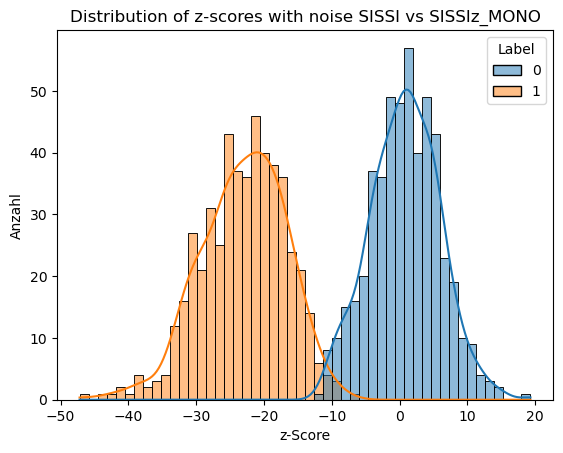
\includegraphics{Histogram SISSI vs SISSIz_mono.png}
    \caption{Histogram SISSI vs SISSIz-mono}
    \label{fig:bar_chart}
\end{figure}

\begin{figure}[H]
    \centering
    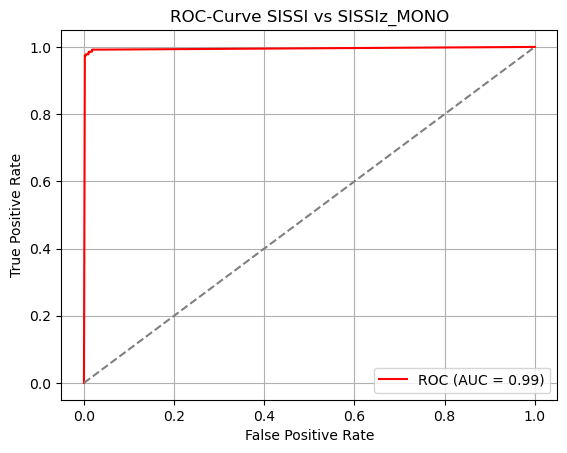
\includegraphics{ROC-CURVE SISSI vs SISSIz_mono.png}
    \caption{ROC-CURVE SISSI vs SISSIz-mono}
    \label{fig:bar_chart}
\end{figure}

\clearpage

\section{SISSI vs SISSIz DI}
\begin{lstlisting}
evaluate_classifier_with_noise(df_sissi, df_sissiz_di, noise_scale=noise_scale_for_all, title_suffix="SISSI vs SISSIZ_DI")
\end{lstlisting}\par

\begin{lstlisting}
 Confusion Matrix:
 [[482  18]
 [ 16 484]]

 Classification Report:
               precision    recall  f1-score   support

           0       0.97      0.96      0.97       500
           1       0.96      0.97      0.97       500

    accuracy                           0.97      1000
   macro avg       0.97      0.97      0.97      1000
weighted avg       0.97      0.97      0.97      1000
\end{lstlisting}\par

\begin{figure}[H]
    \centering
    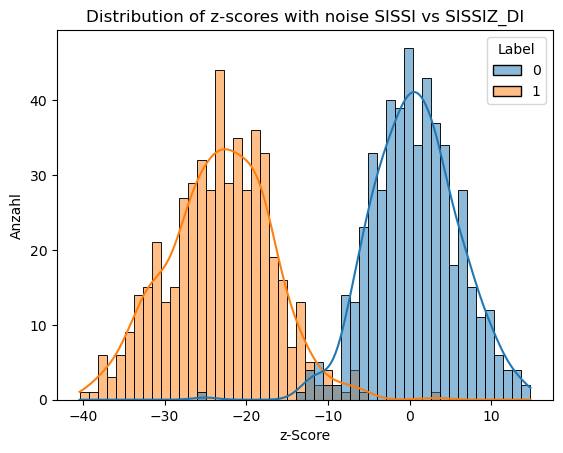
\includegraphics{Histogram SISSI vs SISSIz_di.png}
    \caption{Histogram SISSI vs SISSIz-di}
    \label{fig:bar_chart}
\end{figure}

\begin{figure}[H]
    \centering
    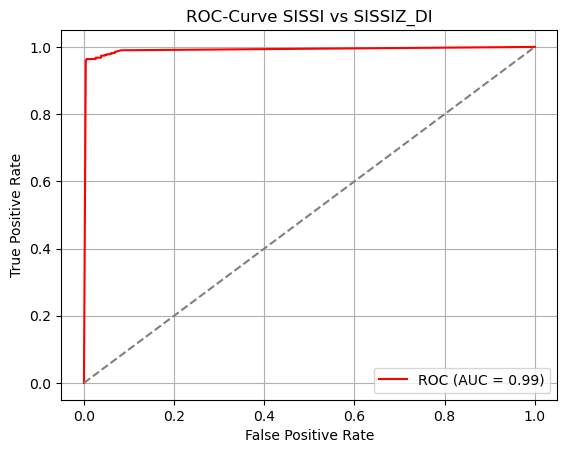
\includegraphics{ROC-CURVE SISSI vs SISSIz_di.png}
    \caption{ROC-CURVE SISSI vs SISSIz-di}
    \label{fig:bar_chart}
\end{figure}

\clearpage

\section{SISSI vs MULTIPERM MONO}
\begin{lstlisting}
evaluate_classifier_with_noise(df_sissi, df_multiperm_mono, noise_scale=noise_scale_for_all, title_suffix="SISSI vs MULTIPERM_MONO")


\begin{lstlisting}
 Confusion Matrix:
 [[467  33]
 [ 32 468]]

 Classification Report:
               precision    recall  f1-score   support

           0       0.94      0.93      0.93       500
           1       0.93      0.94      0.94       500

    accuracy                           0.94      1000
   macro avg       0.94      0.94      0.93      1000
weighted avg       0.94      0.94      0.93      1000
\end{lstlisting}\par

\begin{figure}[H]
    \centering
    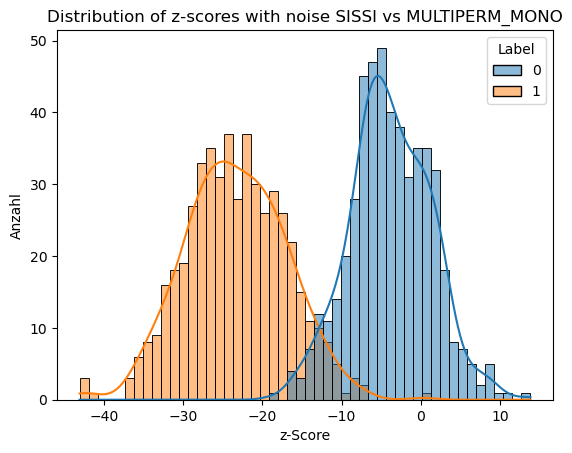
\includegraphics{Histogram SISSI vs MULTIPERM_mono.png}
    \caption{Histogram SISSI vs MULTIPERM-mono}
    \label{fig:bar_chart}
\end{figure}

\begin{figure}[H]
    \centering
    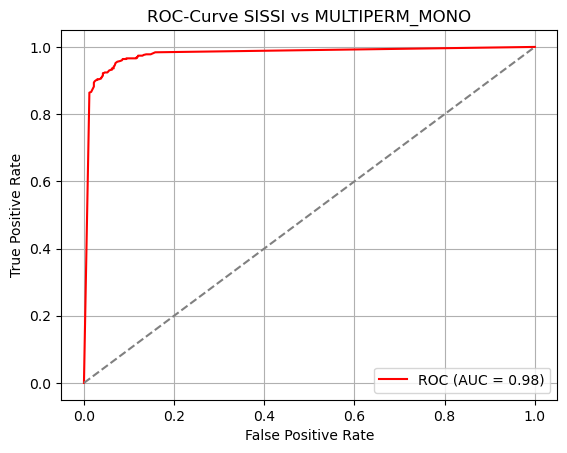
\includegraphics{ROC-CURVE SISSI vs MULTIPERM_mono.png}
    \caption{ROC-CURVE SISSI vs MULTIPERM-mono}
    \label{fig:bar_chart}
\end{figure}

\clearpage

\section{SISSI vs MULTIPERM DI}

\begin{lstlisting}
evaluate_classifier_with_noise(df_sissi, df_multiperm_di, noise_scale=noise_scale_for_all, title_suffix="SISSI vs MULTIPERM_DI")
\end{lstlisting}\par

\begin{lstlisting}
 Confusion Matrix:
 [[475  25]
 [ 31 469]]

 Classification Report:
               precision    recall  f1-score   support

           0       0.94      0.95      0.94       500
           1       0.95      0.94      0.94       500

    accuracy                           0.94      1000
   macro avg       0.94      0.94      0.94      1000
weighted avg       0.94      0.94      0.94      1000
\end{lstlisting}\par

\begin{figure}[H]
    \centering
    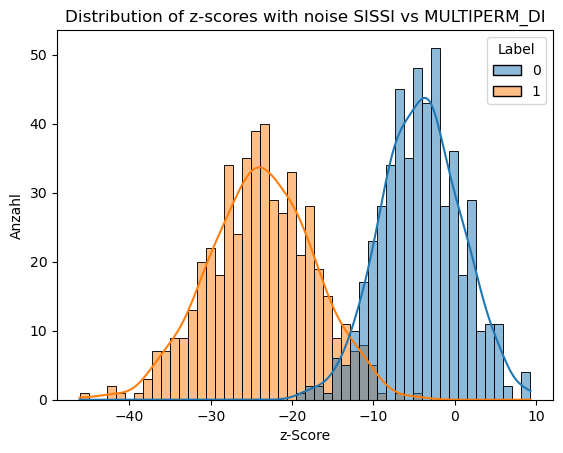
\includegraphics{Histogram SISSI vs MULTIPERM_di.png}
    \caption{Histogram SISSI vs MULTIPERM-di}
    \label{fig:bar_chart}
\end{figure}

\begin{figure}[H]
    \centering
    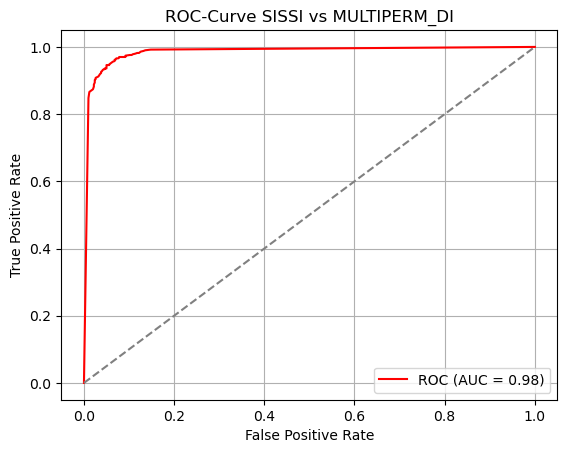
\includegraphics{ROC-CURVE SISSI vs MULTIPERM_di.png}
    \caption{ROC-CURVE SISSI vs MULTIPERM-di}
    \label{fig:bar_chart}
\end{figure}

\clearpage

\section{SISSI vs ALN-SHUFFLE}
\begin{lstlisting}
evaluate_classifier_with_noise(df_sissi, df_aln_shuffle, noise_scale=noise_scale_for_all, title_suffix="SISSI vs ALN-SHUFFLE")
\end{lstlisting}\par

\begin{lstlisting}
 Confusion Matrix:
 [[399 101]
 [ 97 403]]

 Classification Report:
               precision    recall  f1-score   support

           0       0.80      0.80      0.80       500
           1       0.80      0.81      0.80       500

    accuracy                           0.80      1000
   macro avg       0.80      0.80      0.80      1000
weighted avg       0.80      0.80      0.80      1000
\end{lstlisting}\par

\begin{figure}[H]
    \centering
    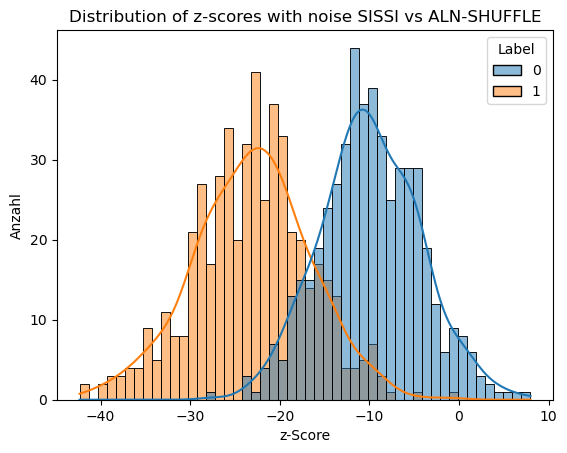
\includegraphics{Histogram SISSI vs ALN-SHUFFLE.png}
    \caption{Histogram SISSI vs ALN-SHUFFLE}
    \label{fig:bar_chart}
\end{figure}

\begin{figure}[H]
    \centering
    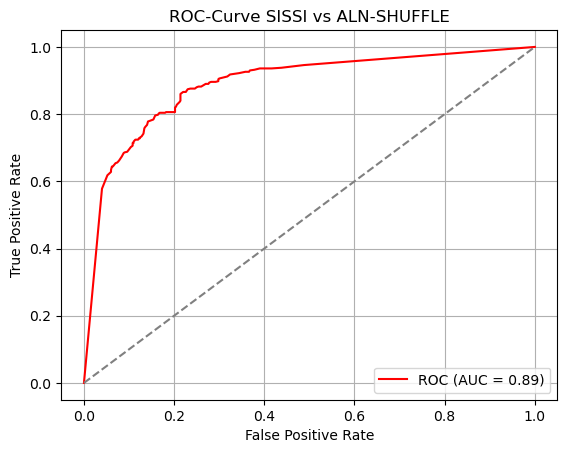
\includegraphics{ROC-CURVE SISSI vs ALN-SHUFFLE.png}
    \caption{ROC-CURVE SISSI vs ALN-SHUFFLE}
    \label{fig:bar_chart}
\end{figure}

\clearpage

\section{Summary of the Results}

The ROC curve compares the true positive rate against the false positive rate for different threshold values. The AUC value (Area Under Curve) measures the quality of the separation between the classes.\vspace{1em}

Die beste Klassifikationsleistung wurde bei der Gegenüberstellung von SISSI und SISSIz MONO erzielt. Das Modell erreichte eine Accuracy von 98 Prozent bei einem F1-Score von 0{,}98 für beide Klassen. Die Anzahl an Fehlklassifikationen war mit lediglich 9 False Positives und 7 False Negatives minimal, was auf eine sehr klare Trennbarkeit der beiden Datenquellen hinweist. \vspace{1em}

The ROC curve compares the true positive rate against the false positive rate for different threshold values. The AUC value (Area Under Curve) measures the quality of the separation between the classes. \vspace{1em}

The control groups based on MULTIPERM achieved an accuracy of 94 percent with a mean F1 score of 0{,}94. The MULTIPERM MONO and MULTIPERM DI configurations delivered very similar results, with MULTIPERM DI showing a minimally better recall value for the positive class. Overall, however, these values indicate that MULTIPERM-based shuffling is structurally closer to the SISSI data than the SISSIz controls. \vspace{1em}

A significantly lower classification quality was observed in the last comparison with ALN-SHUFFLE (Accuracy 80 percent, F1-Score 0{,}80). However, the high number of misclassifications (101 FP, 97 FN) suggests a strong structural similarity to the positive class, which made separation by the model considerably more difficult. \vspace{1em}

In summary, the SISSIz MONO method provides the clearest separation from the original structure and can therefore be identified as the most effective negative control method within this classification framework. It provides a well-distinguishable contrast image, which is ideally suited for further analysis or validation steps. \vspace{1em}

\clearpage

\section{SPOT-RNA2}
I am currently installing SPOT-RNA2 on the FH AI server but the databases are still missing and should be fully downloaded in 2 days.

\section{DeepFoldRNA}

I installed DeepFoldRNA on the FH AI server, but encountered an issue during execution: DeepFoldRNA only accepts single FASTA sequences. After reducing the input to individual sequences, the execution started successfully. However, the process took more than 12 hours and eventually stopped without producing meaningful results. Due to this, I have decided to replace DeepFoldRNA with MXfold2.


\section{RNA secondary structure prediction using deep learning with thermodynamic integration\href{https://doi.org/10.1038/s41467-021-21194-4}{\textbf{[1]}}\href{https://github.com/mxfold/mxfold2?tab=readme-ov-file}{\textbf{[2]}}}

\textbf{Introduction}\par
Accurate prediction of RNA secondary structure is essential for understanding the function of non-coding RNAs. Traditional models use free energy minimization, while recent approaches have applied deep learning. However, deep learning often overfits to the training data, limiting generalizability. The aim of this study is to integrate deep learning with thermodynamic models to achieve a more robust and generalizable RNA secondary structure predictor.\vspace{1em}

\textbf{Methods}\par
The authors developed MXfold2, which computes folding scores using a deep neural network and integrates these with experimentally derived thermodynamic parameters from Turner's model.
\vspace{1em}

Key innovations include:
\begin{itemize}
        \item Thermodynamic Integration: Combining deep learning–based scores with known free energy rules.
        \item Thermodynamic Regularization: A loss term that forces the neural network’s outputs to align with thermodynamic energy predictions. The model uses bidirectional LSTMs and convolutional neural networks to capture both local and long-range dependencies in RNA sequences.\\[0.5em]
\end{itemize} 

\textbf{Results}\par

MXfold2 was benchmarked against CONTRAfold, RNAfold, SPOT-RNA, and E2Efold using:

\begin{itemize}
        \item Sequence-wise Cross-validation: MXfold2 achieved significantly higher accuracy.
        \item Family-wise Cross-validation: Unlike other models, MXfold2 maintained high performance and avoided overfitting.
        \item Independent Test Sets: The method outperformed competitors even on previously unseen RNA families. Moreover, MXfold2 was computationally efficient and scalable to longer sequences. \\[0.5em]
\end{itemize} 

\textbf{Discussion}\par
The authors emphasize that integrating data-driven learning with physics-based modeling yields synergistic benefits. The approach captures the adaptability of deep learning while maintaining consistency with physical principles. This duality enhances both accuracy and generalization. They suggest this framework could be extended to related problems like RNA tertiary structure prediction and RNA-protein interactions.\vspace{1em}

\textbf{Conclusion}\par
MXfold2 represents a significant step forward in RNA bioinformatics. By combining thermodynamic modeling with deep learning, it delivers accurate and generalizable RNA secondary structure predictions—crucial for studying novel non-coding RNAs.\vspace{1em}


\section{References}
\begin{itemize}
    \item[\textbf{[1]}] \url{https://doi.org/10.1038/s41467-021-21194-4} \par
    \item[\textbf{[2]}] \url{https://github.com/mxfold/mxfold2?tab=readme-ov-file} \par
\end{itemize}

\end{large}
\end{document}


Summary KW18 - KW22

\documentclass{article}
\usepackage{graphicx} % Required for inserting images
\usepackage{hyperref}
\usepackage{setspace}
\usepackage{listings}
\usepackage{float}
\usepackage[font=small,labelfont=bf]{caption}
\usepackage[a4paper, margin=1in]{geometry}
\usepackage{setspace}  
\onehalfspacing
\usepackage{hyperref}
\usepackage{xcolor}
\usepackage{graphicx}
\usepackage{caption}
\usepackage{subcaption}
\hypersetup{
    colorlinks=true, 
    linkcolor=blue, 
    urlcolor=blue,  
}

\usepackage{listings}
\usepackage{xcolor}

\lstset{
    language=Python,
    basicstyle=\ttfamily\small,
    keywordstyle=\bfseries\color{blue},
    commentstyle=\itshape\color{gray},
    stringstyle=\color{orange},
    showstringspaces=false,
    numbers=left,
    numberstyle=\tiny,
    breaklines=true,
    frame=single
    aboveskip=1em,
    belowskip=1em
}


% Einstellungen für Code Listings
\lstset{
basicstyle=\ttfamily\small,
breaklines=true,
frame=single
}

\setlength{\parindent}{0pt}
\setlength{\textfloatsep}{0pt}

\title{KW18 - KW22 Summary}
\author{Stefan Redl}
\begin{document}
\maketitle

\begin{large}

\section{Results of SISSIz Prediction}

\subsection{SISSIz Boxplot}
\begin{figure}[H]
    \centering
    \includegraphics[scale=0.7]{Boxplot SISSIz z-score.png}
    \caption{Boxplot SISSIz z-score}
    \label{fig:bar_chart}
\end{figure}

The boxplots clearly show the selectivity of the different models. In particular, SISSIz-mono and SISSIz-di stand out as the most effective in destroying the RNA secondary structure. In contrast, the other models showed little to no destructive effect. The worst result was achieved by ALN-Shuffle, which could hardly affect the structure of the RNA.

\subsection{SISSIz Histograms}

\begin{figure}[H]
    \centering
    \begin{subfigure}[b]{0.48\textwidth}
        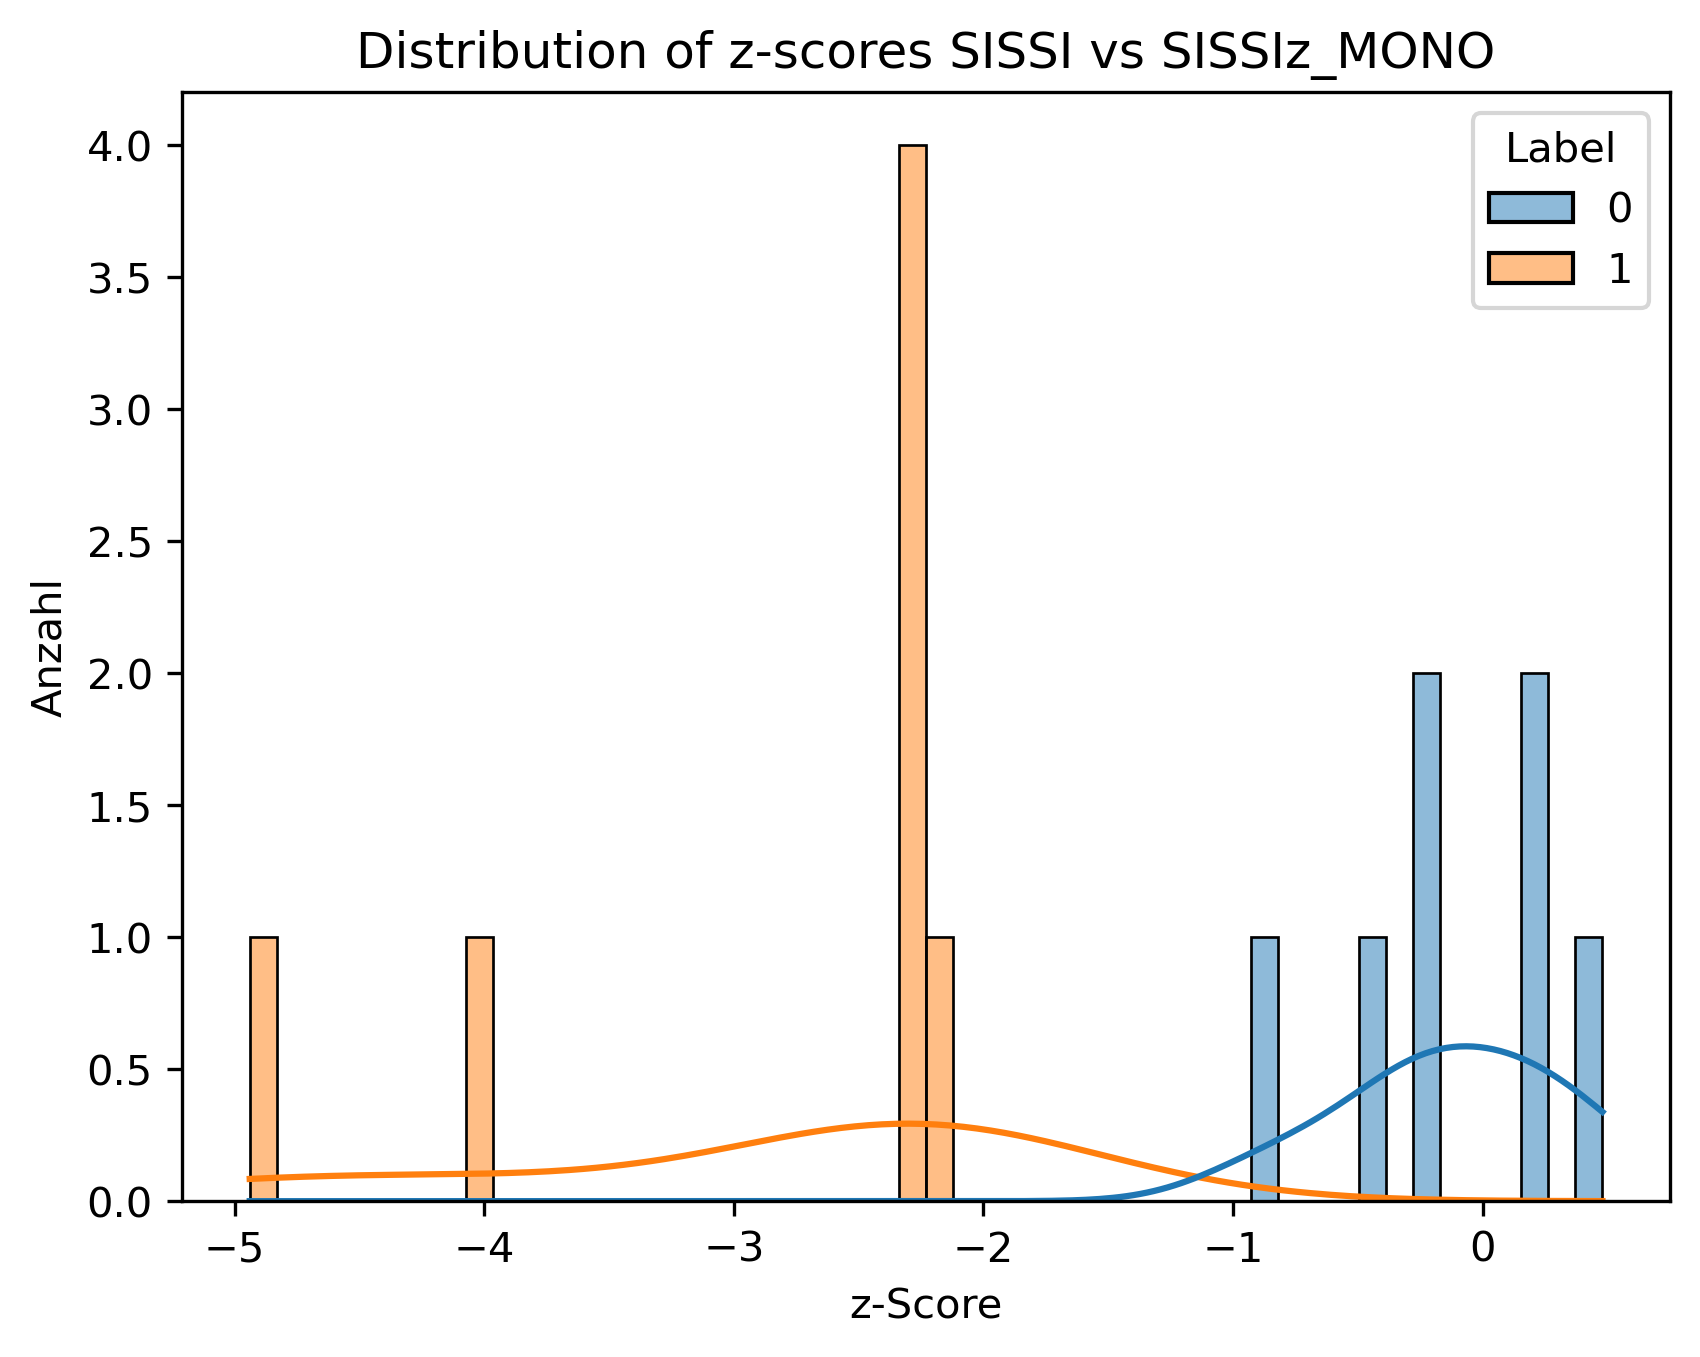
\includegraphics[width=\textwidth]{SISSIz_Histogram_SISSI_vs_SISSIz_MONO.png}
        \caption{SISSI vs SISSIz-mono}
        \label{fig:hist_sissiz_mono}
    \end{subfigure}
    \hfill
    \begin{subfigure}[b]{0.48\textwidth}
        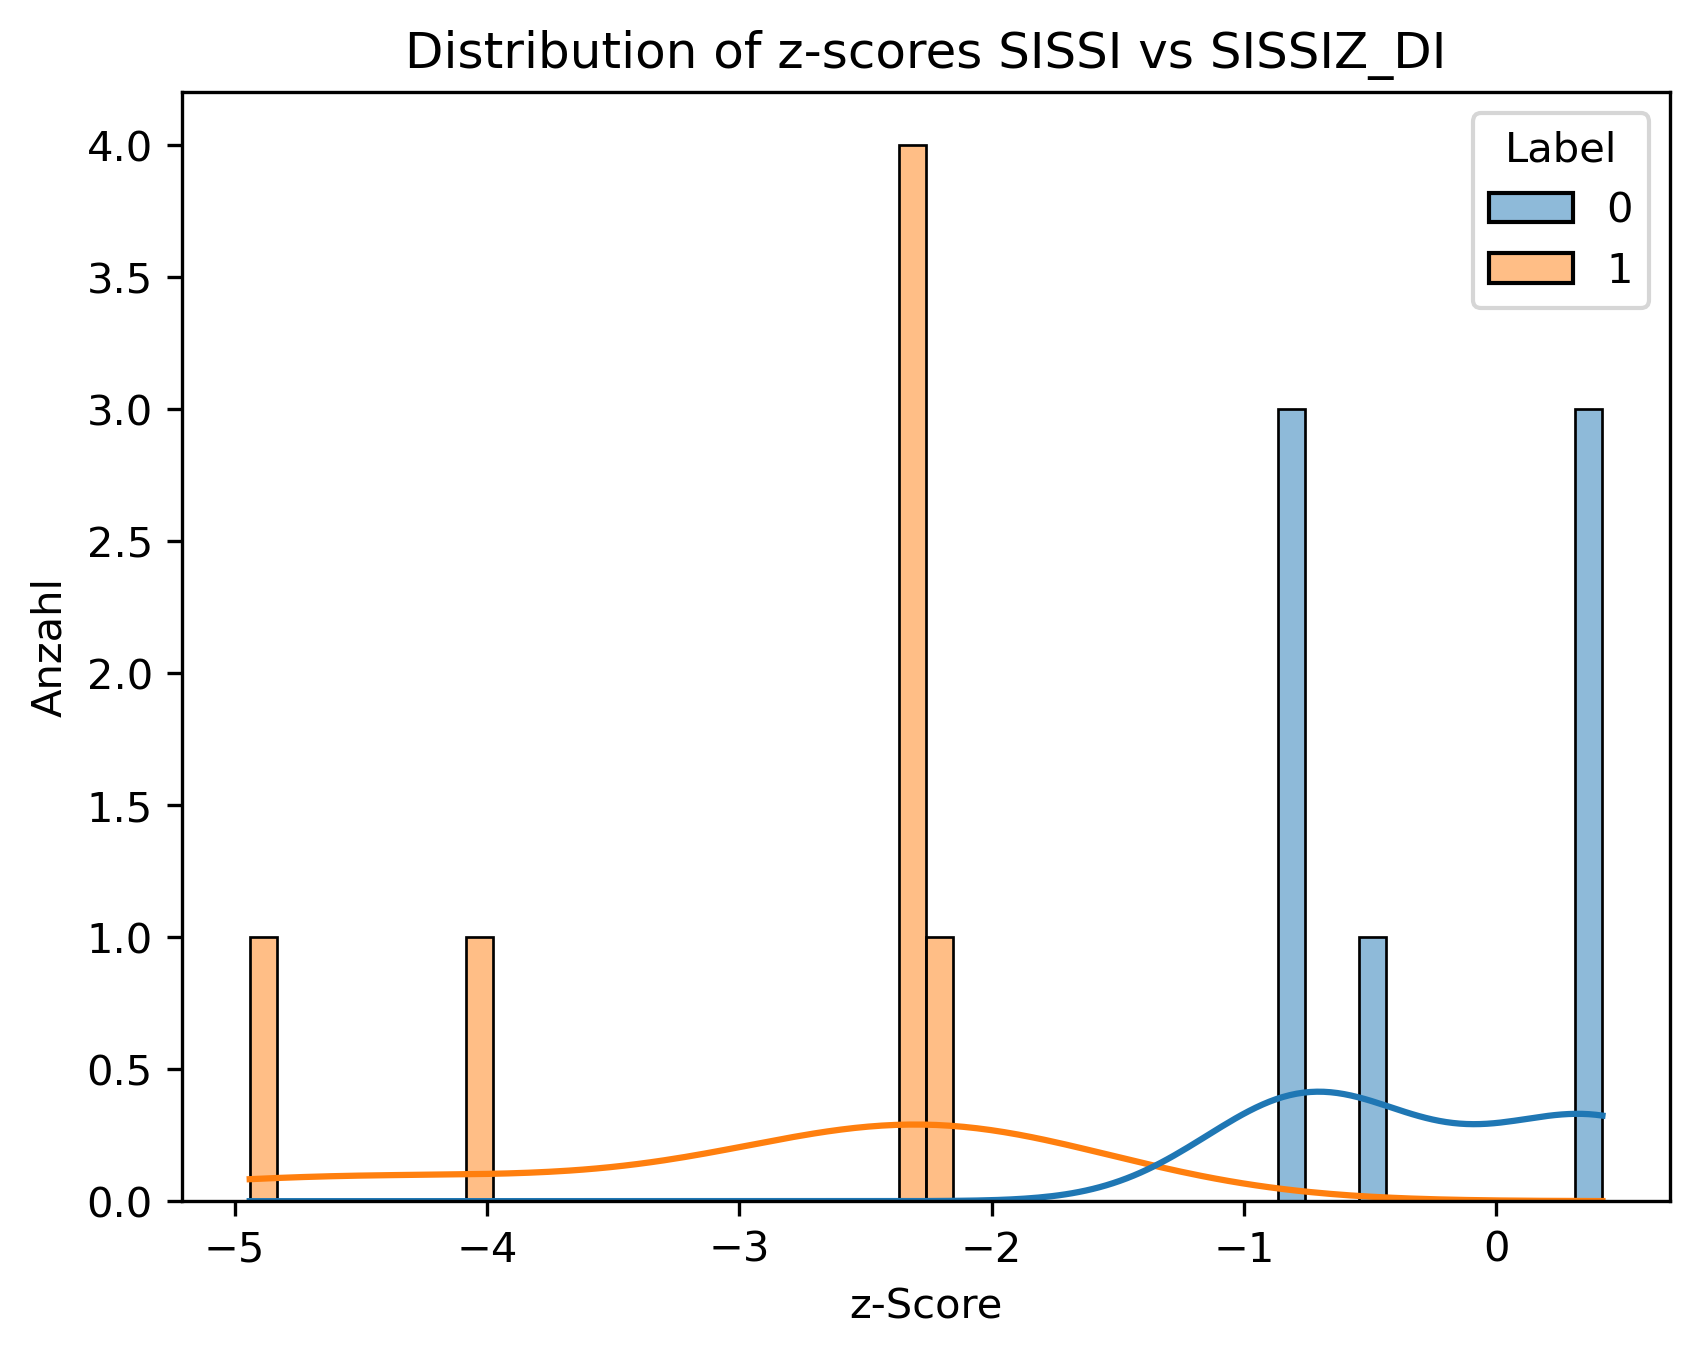
\includegraphics[width=\textwidth]{SISSIz_Histogram_SISSI_vs_SISSIZ_DI.png}
        \caption{SISSI vs SISSIz-di}
        \label{fig:hist_sissiz_di}
    \end{subfigure}
    \vspace{1em}
    
    \begin{subfigure}[b]{0.48\textwidth}
        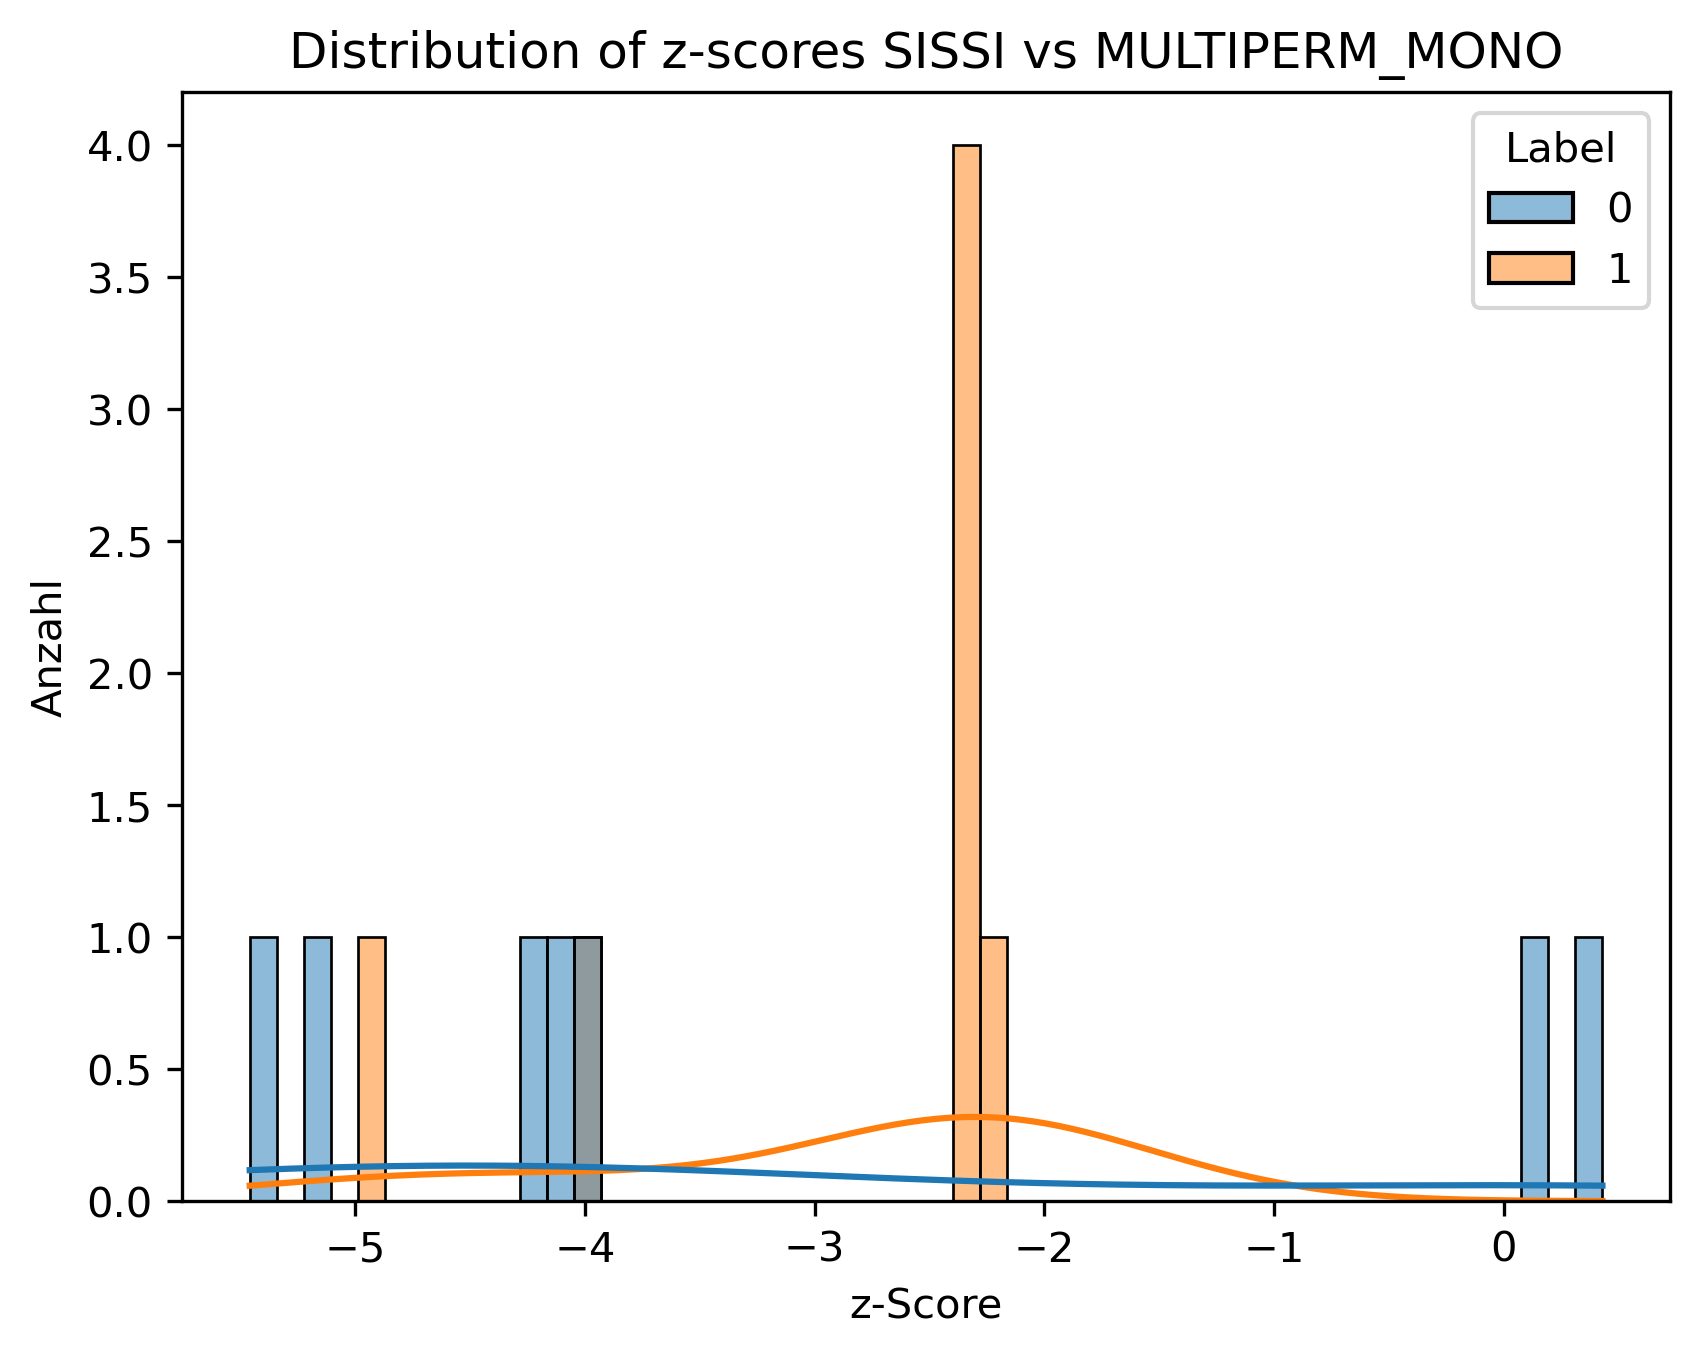
\includegraphics[width=\textwidth]{SISSIz_Histogram_SISSI_vs_MULTIPERM_MONO.png}
        \caption{SISSI vs MULTIPERM-mono}
        \label{fig:hist_multiperm_mono}
    \end{subfigure}
    \hfill
    \begin{subfigure}[b]{0.48\textwidth}
        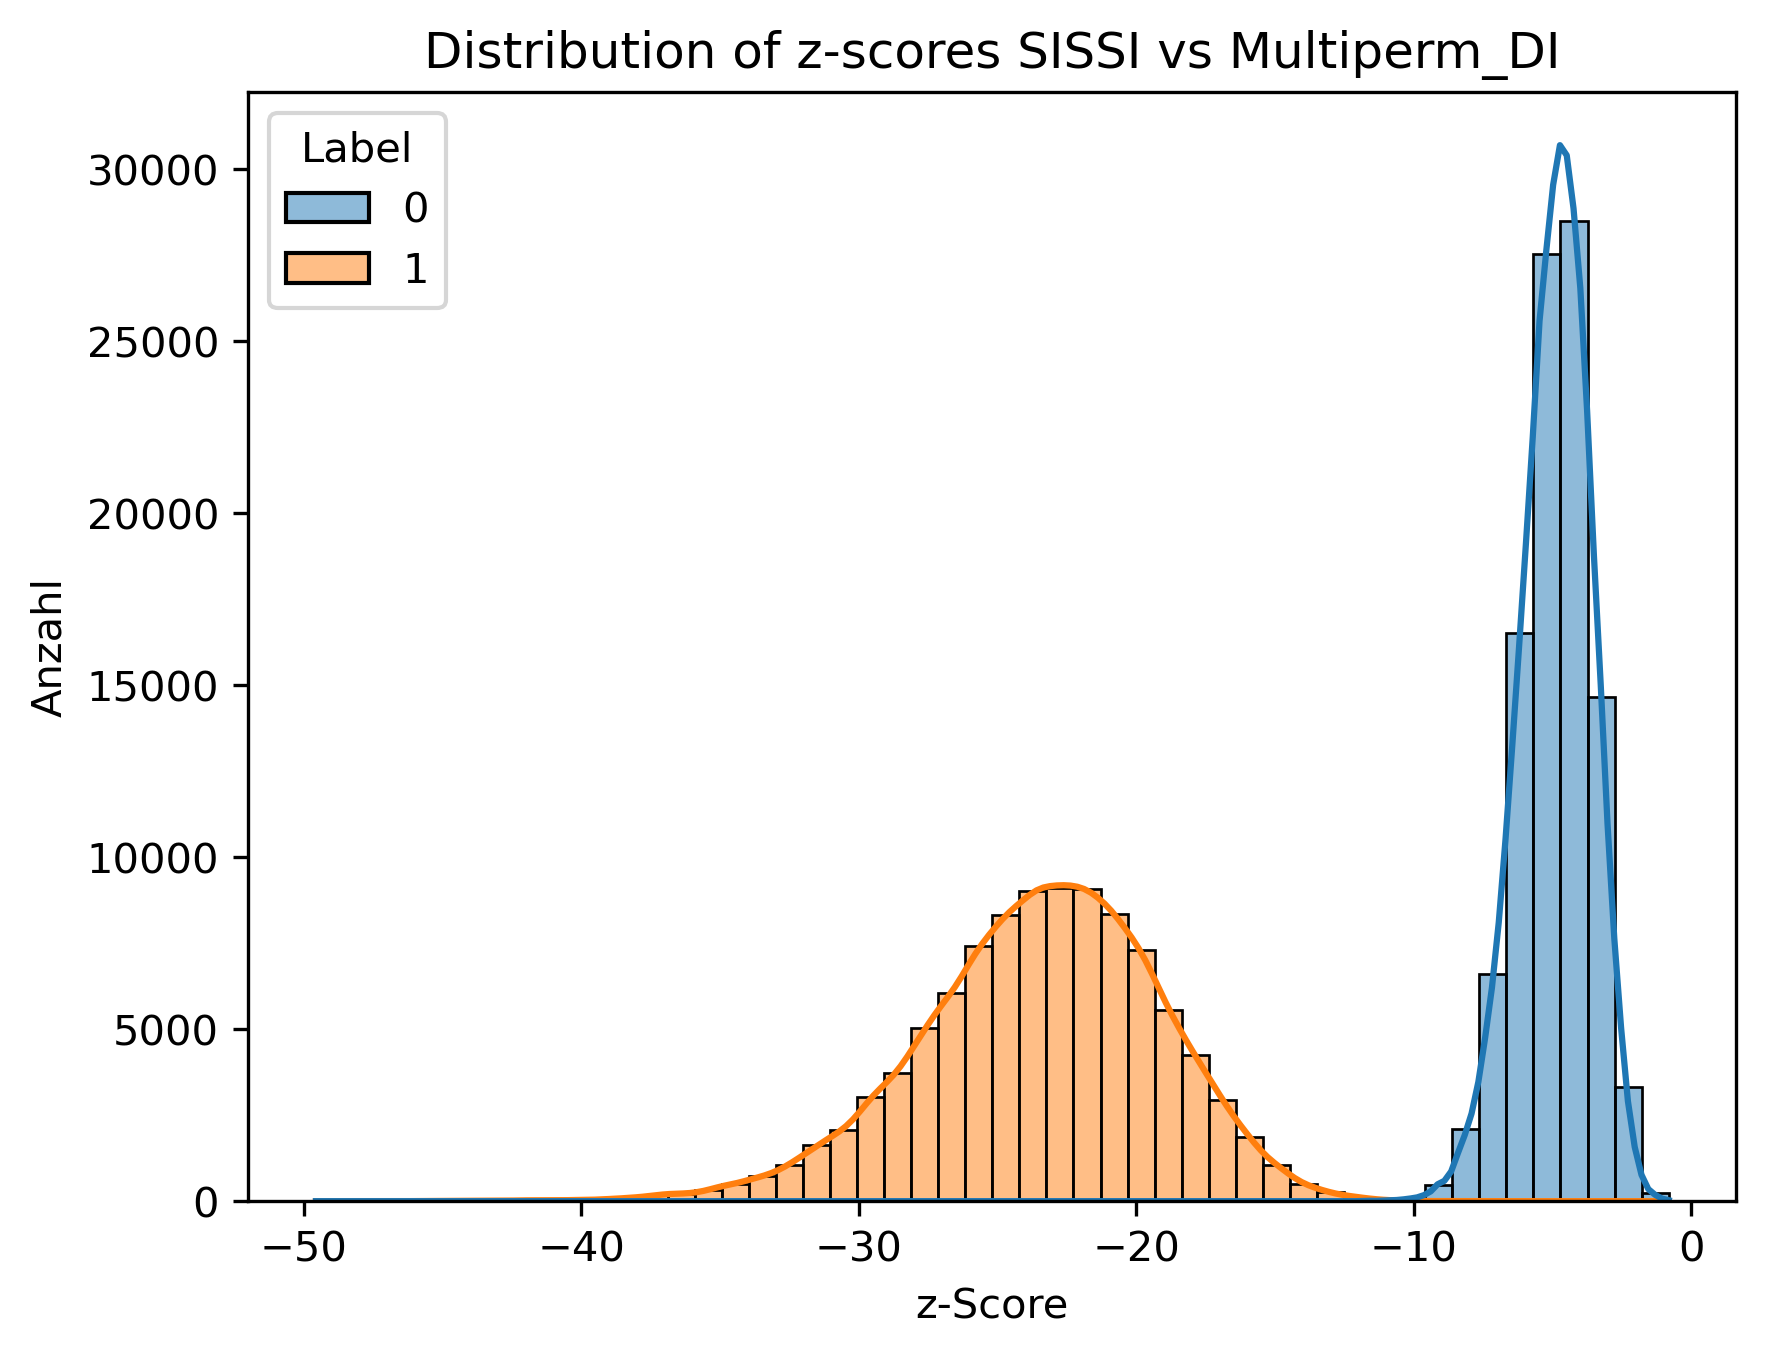
\includegraphics[width=\textwidth]{SISSIz_Histogram_SISSI_vs_MULTIPERM_DI.png}
        \caption{SISSI vs MULTIPERM-di}
        \label{fig:hist_multiperm_di}
    \end{subfigure}
    \vspace{1em}
    
    \begin{subfigure}[b]{0.48\textwidth}
        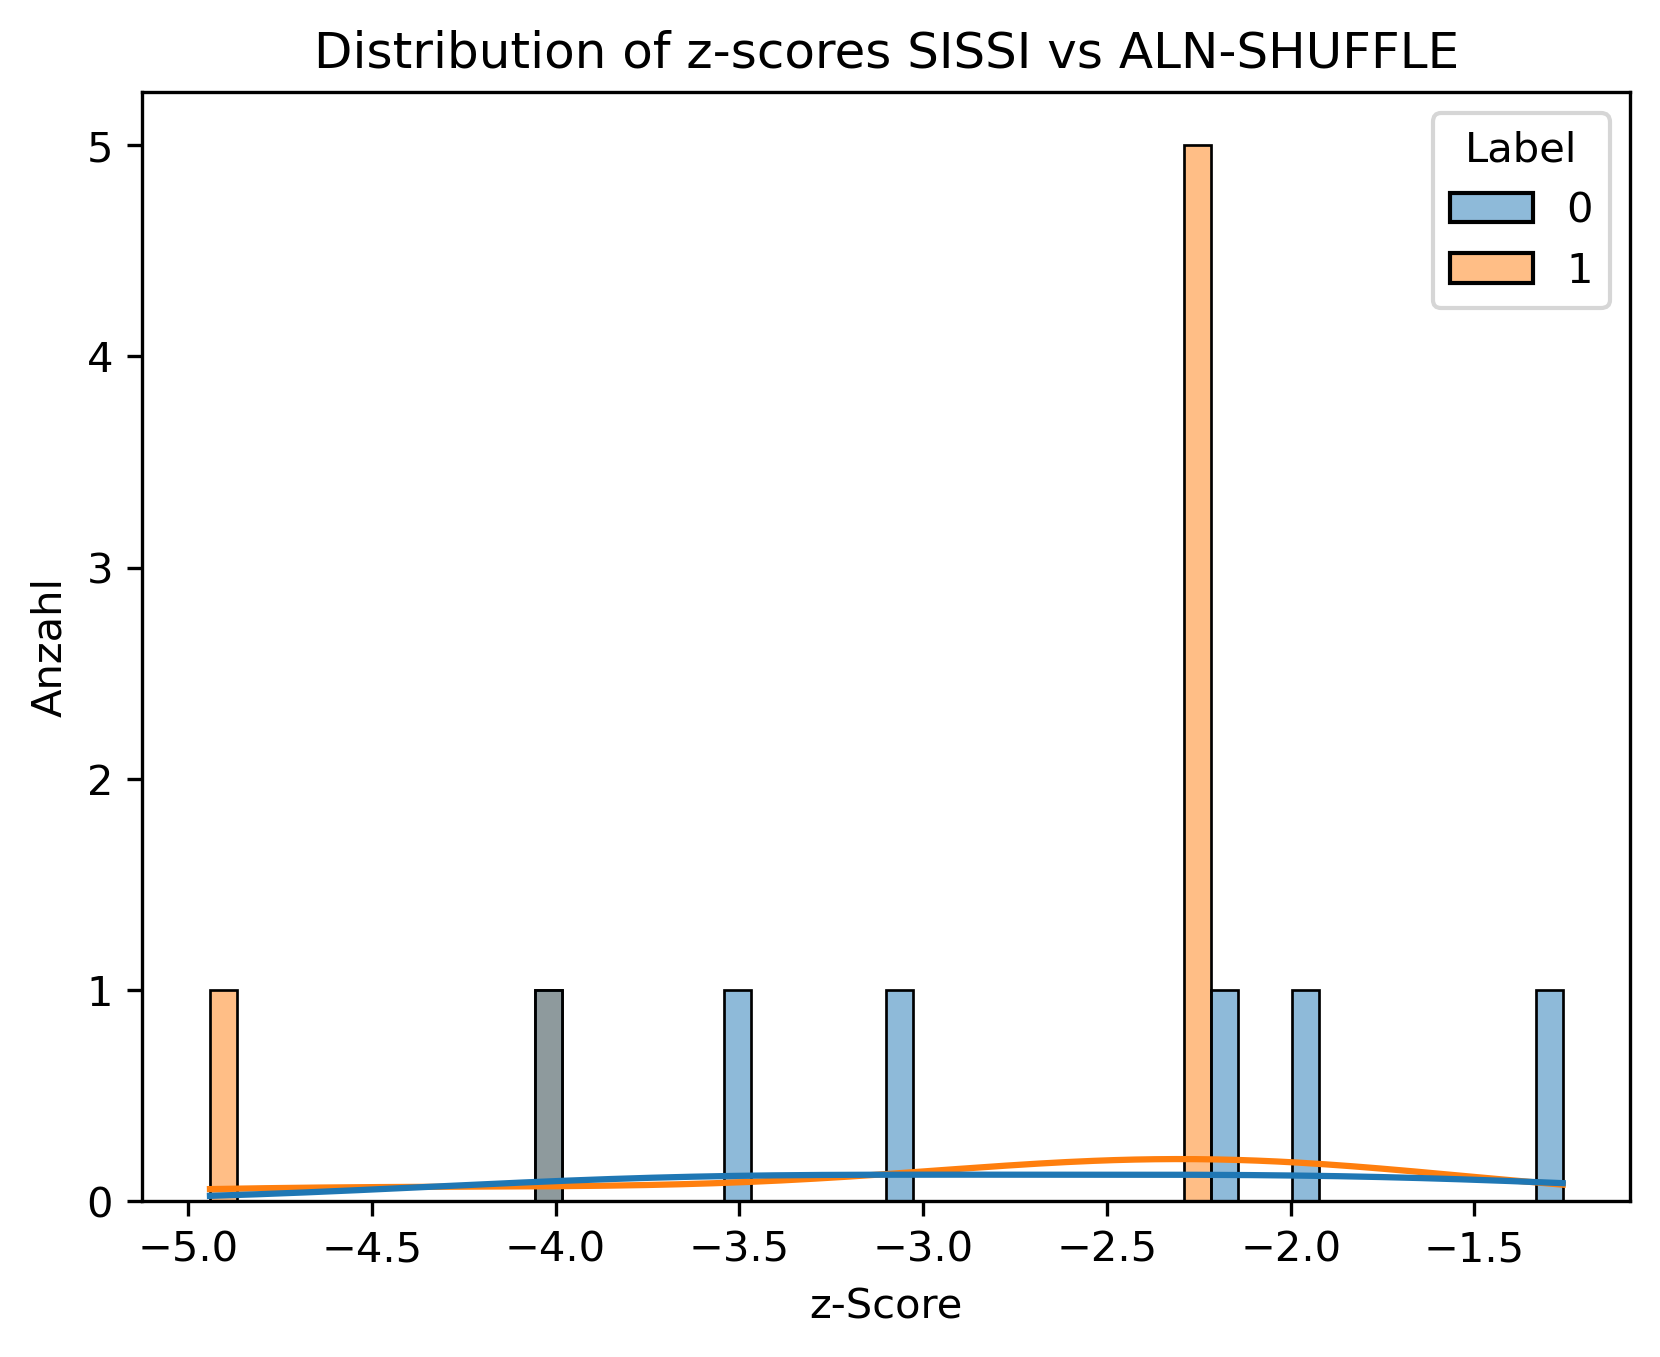
\includegraphics[width=\textwidth]{SISSIz_Histogram_SISSI_vs_ALN-SHUFFLE.png}
        \caption{SISSI vs ALN-SHUFFLE}
        \label{fig:hist_aln_shuffle}
    \end{subfigure}

    \caption{Histograms from SISSIz prediction}
    \label{fig:all_histograms}
\end{figure}

The histograms also confirm the results from the boxplots: The separability of the models is easily recognizable, and again \textit{SISSIz-mono} and \textit{SISSIz-di} show the best performance. \vspace{1em}

\subsection{SISSIz Confusion Matrix}

\begin{figure}[H]
    \centering
    \begin{subfigure}[b]{0.48\textwidth}
        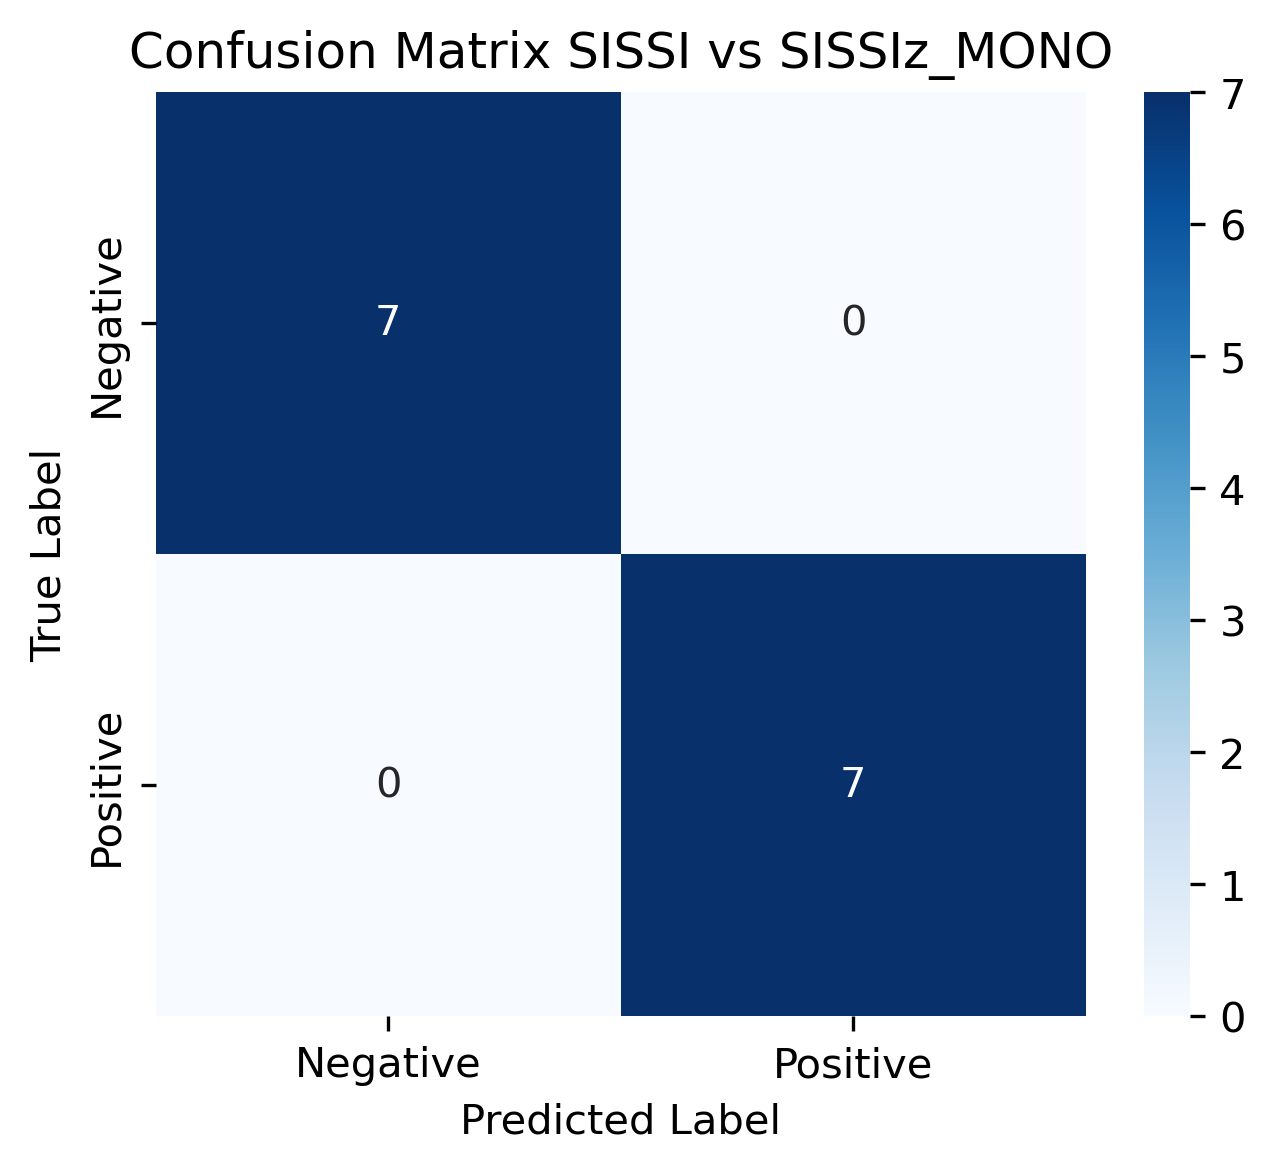
\includegraphics[width=\textwidth]{SISSIz_Confusion_Matrix_SISSI_vs_SISSIz_MONO.png}
        \caption{SISSI vs SISSIz-mono}
        \label{fig:confusion_sissiz_mono}
    \end{subfigure}
    \hfill
    \begin{subfigure}[b]{0.48\textwidth}
        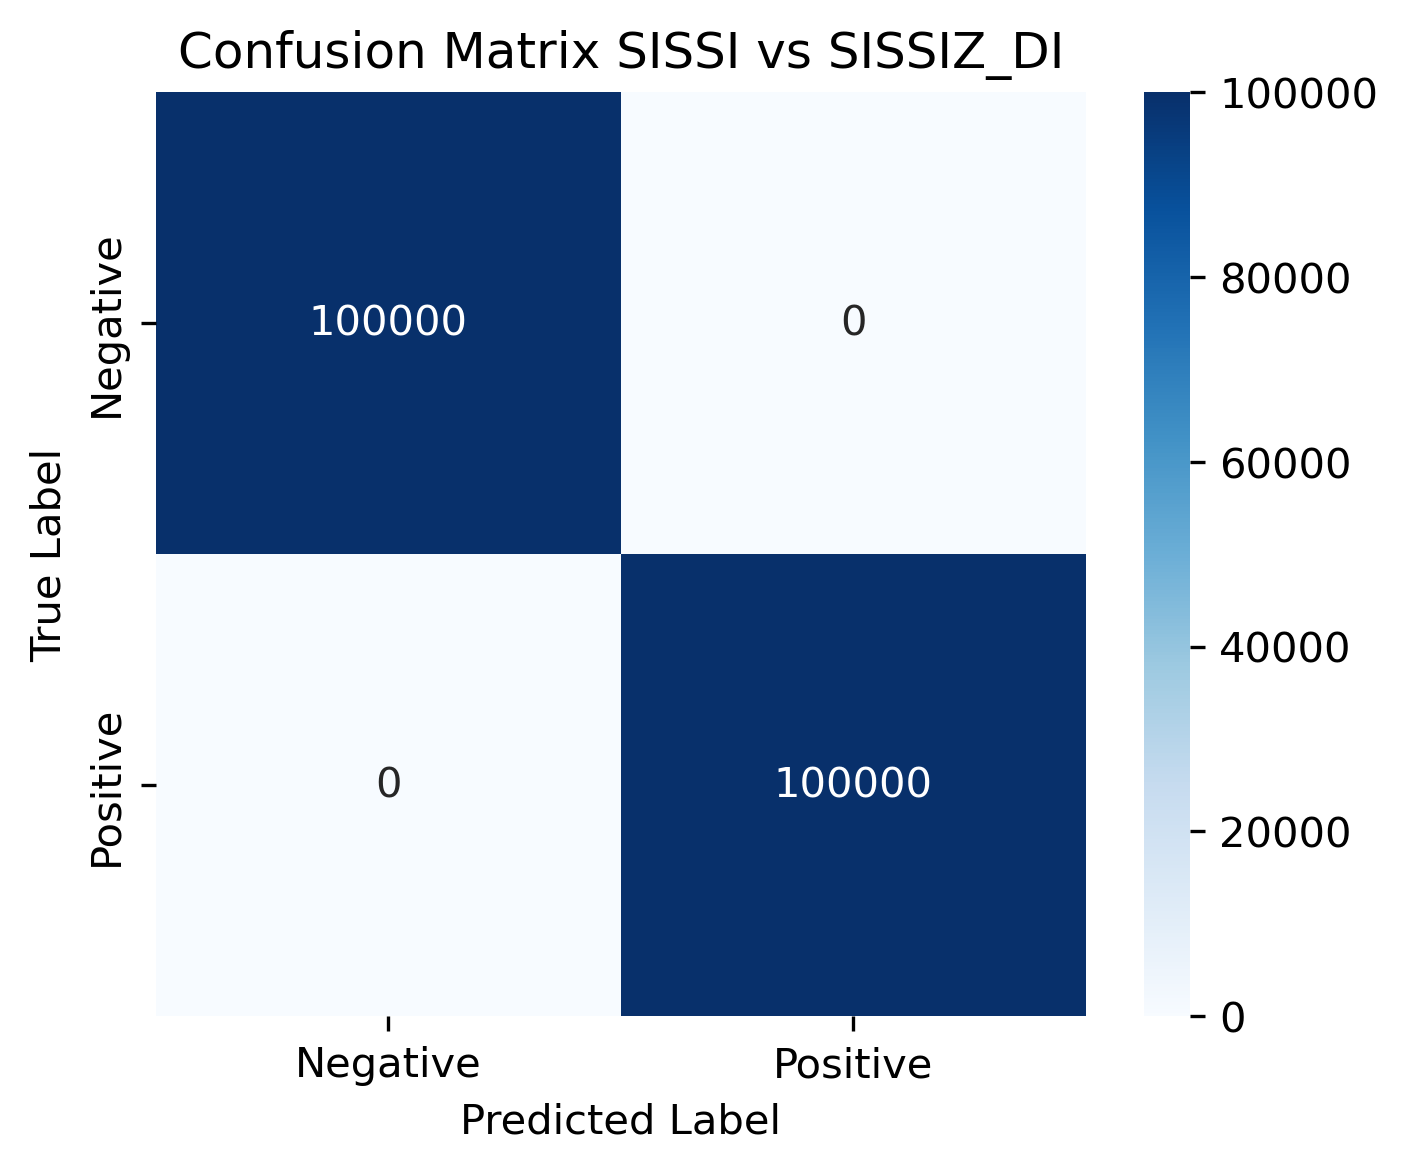
\includegraphics[width=\textwidth]{SISSIz_Confusion_Matrix_SISSI_vs_SISSIZ_DI.png}
        \caption{SISSI vs SISSIz-di}
        \label{fig:confusion_sissiz_di}
    \end{subfigure}
    \vspace{1em}
    
    \begin{subfigure}[b]{0.48\textwidth}
        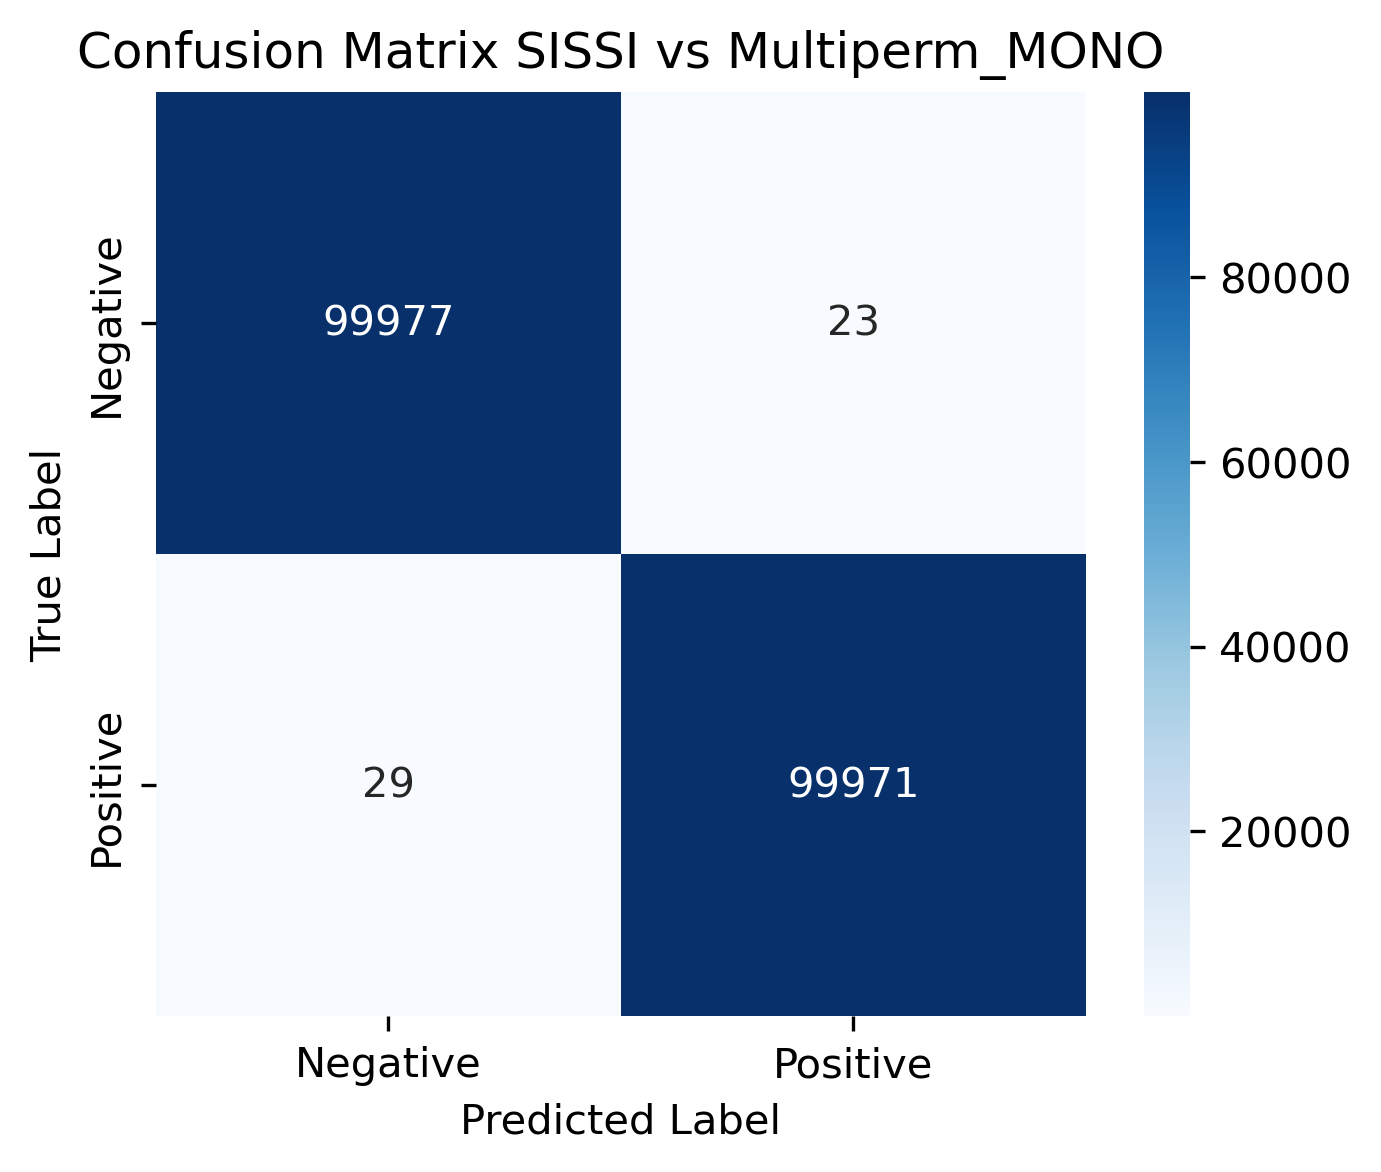
\includegraphics[width=\textwidth]{SISSIz_Confusion_Matrix_SISSI_vs_MULTIPERM_MONO.png}
        \caption{SISSI vs MULTIPERM-mono}
        \label{fig:confusion_multiperm_mono}
    \end{subfigure}
    \hfill
    \begin{subfigure}[b]{0.48\textwidth}
        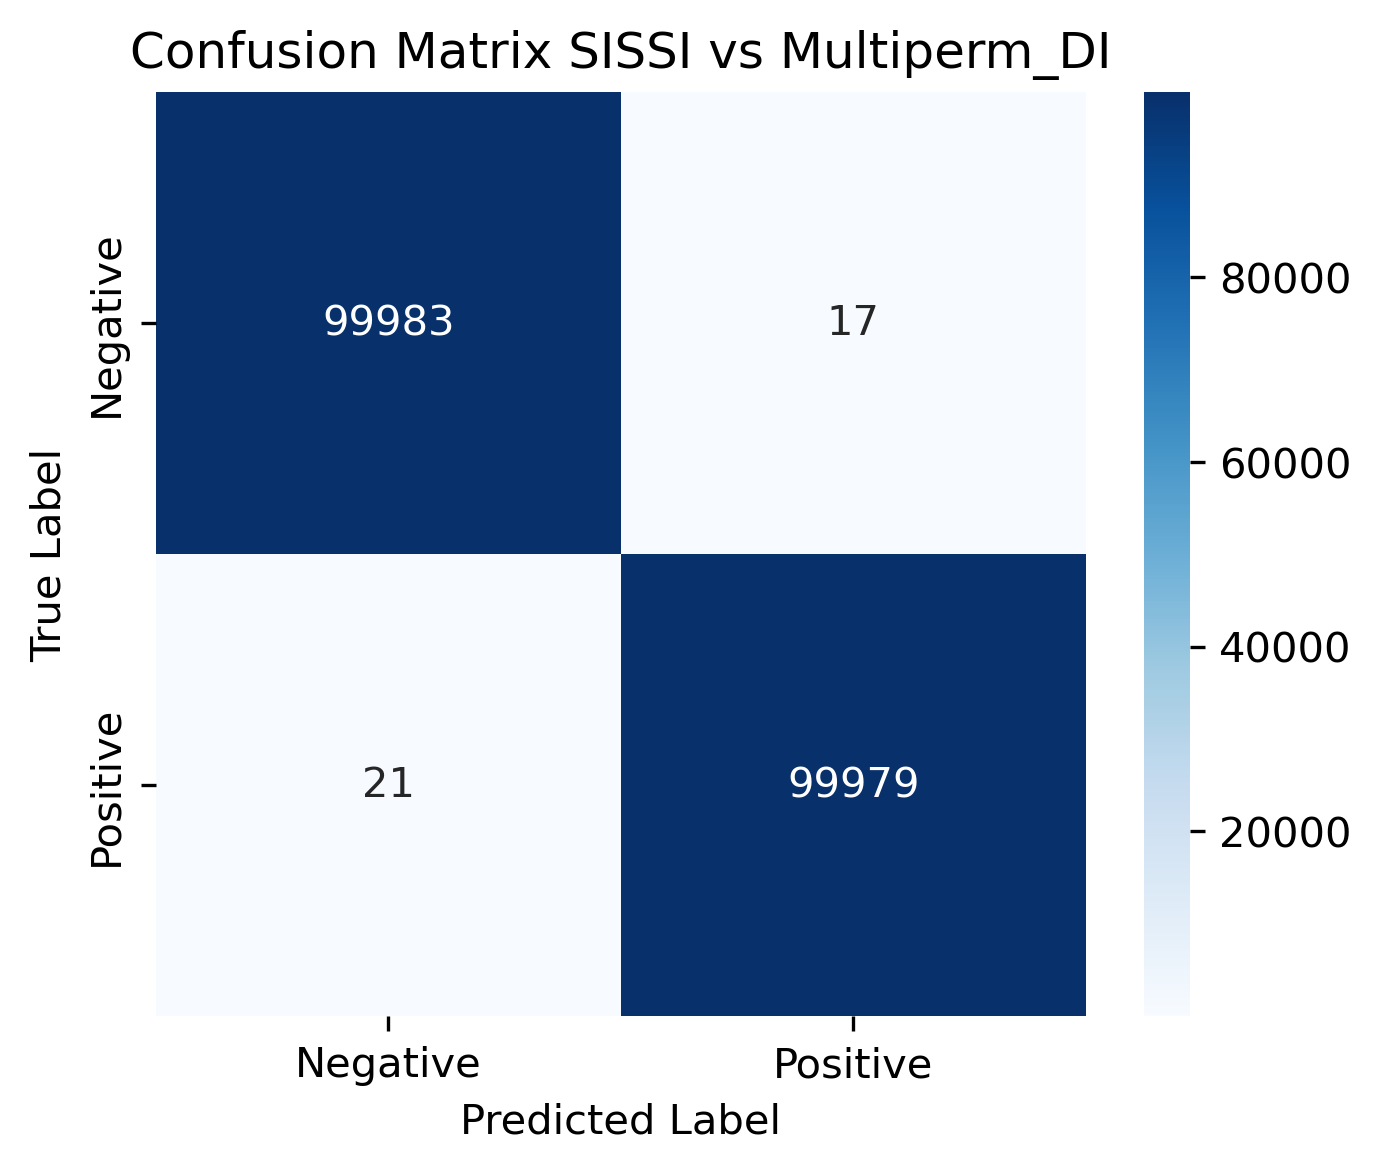
\includegraphics[width=\textwidth]{SISSIz_Confusion_Matrix_SISSI_vs_MULTIPERM_DI.png}
        \caption{SISSI vs MULTIPERM-di}
        \label{fig:confusion_multiperm_di}
    \end{subfigure}
    \vspace{1em}
    
    \begin{subfigure}[b]{0.48\textwidth}
        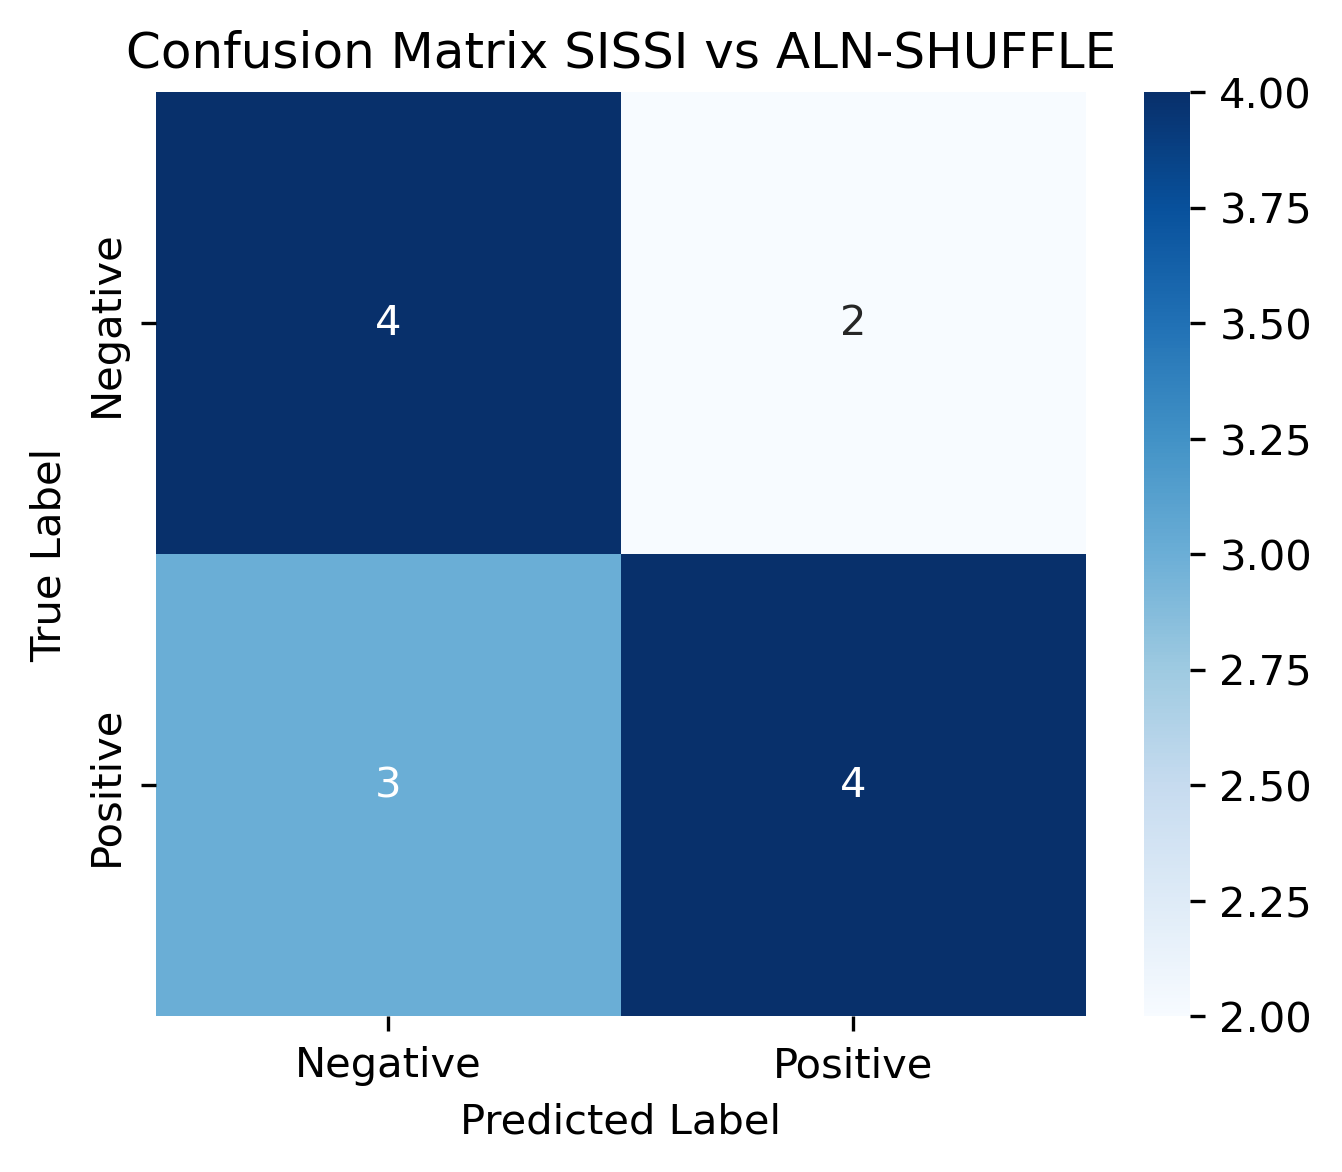
\includegraphics[width=\textwidth]{SISSIz_Confusion_Matrix_SISSI_vs_ALN-SHUFFLE.png}
        \caption{SISSI vs ALN-SHUFFLE}
        \label{fig:confusion_aln_shuffle}
    \end{subfigure}

    \caption{Confusion Matrix from SISSIz prediction}
    \label{fig:all_confusionograms}
\end{figure}

The evaluation of the confusion matrices illustrates the concrete separation performance of the respective models.\vspace{1em}

The SISSIz-mono and SISSIz-di models each achieved 0 false positives and 0 false negatives like in the Figure 3 (a) and (b), which indicates an almost perfect separation of the classes. These results indicate excellent separability between the original and the negatively controlled RNA structures.\vspace{1em}

In contrast, the multiperm-mono and multiperm-di models showed solid classification performance, but with some misclassifications:\vspace{1em}

Multiperm-mono Figure 3 (c): 23 false positives, 29 false negatives

Multiperm-di Figure 3 (d): 17 false positives, 21 false negatives
\vspace{1em}

The worst separability was found in the Aln-Shuffle Figure 3 (e) scenario, with 3877 false positives and 5327 false negatives. These high misclassification numbers illustrate the difficulty of reliably distinguishing this model from the original structure.\vspace{1em}

\subsection{SISSIz ROC-Kurven}

\begin{figure}[H]
    \centering
    \begin{subfigure}[b]{0.48\textwidth}
        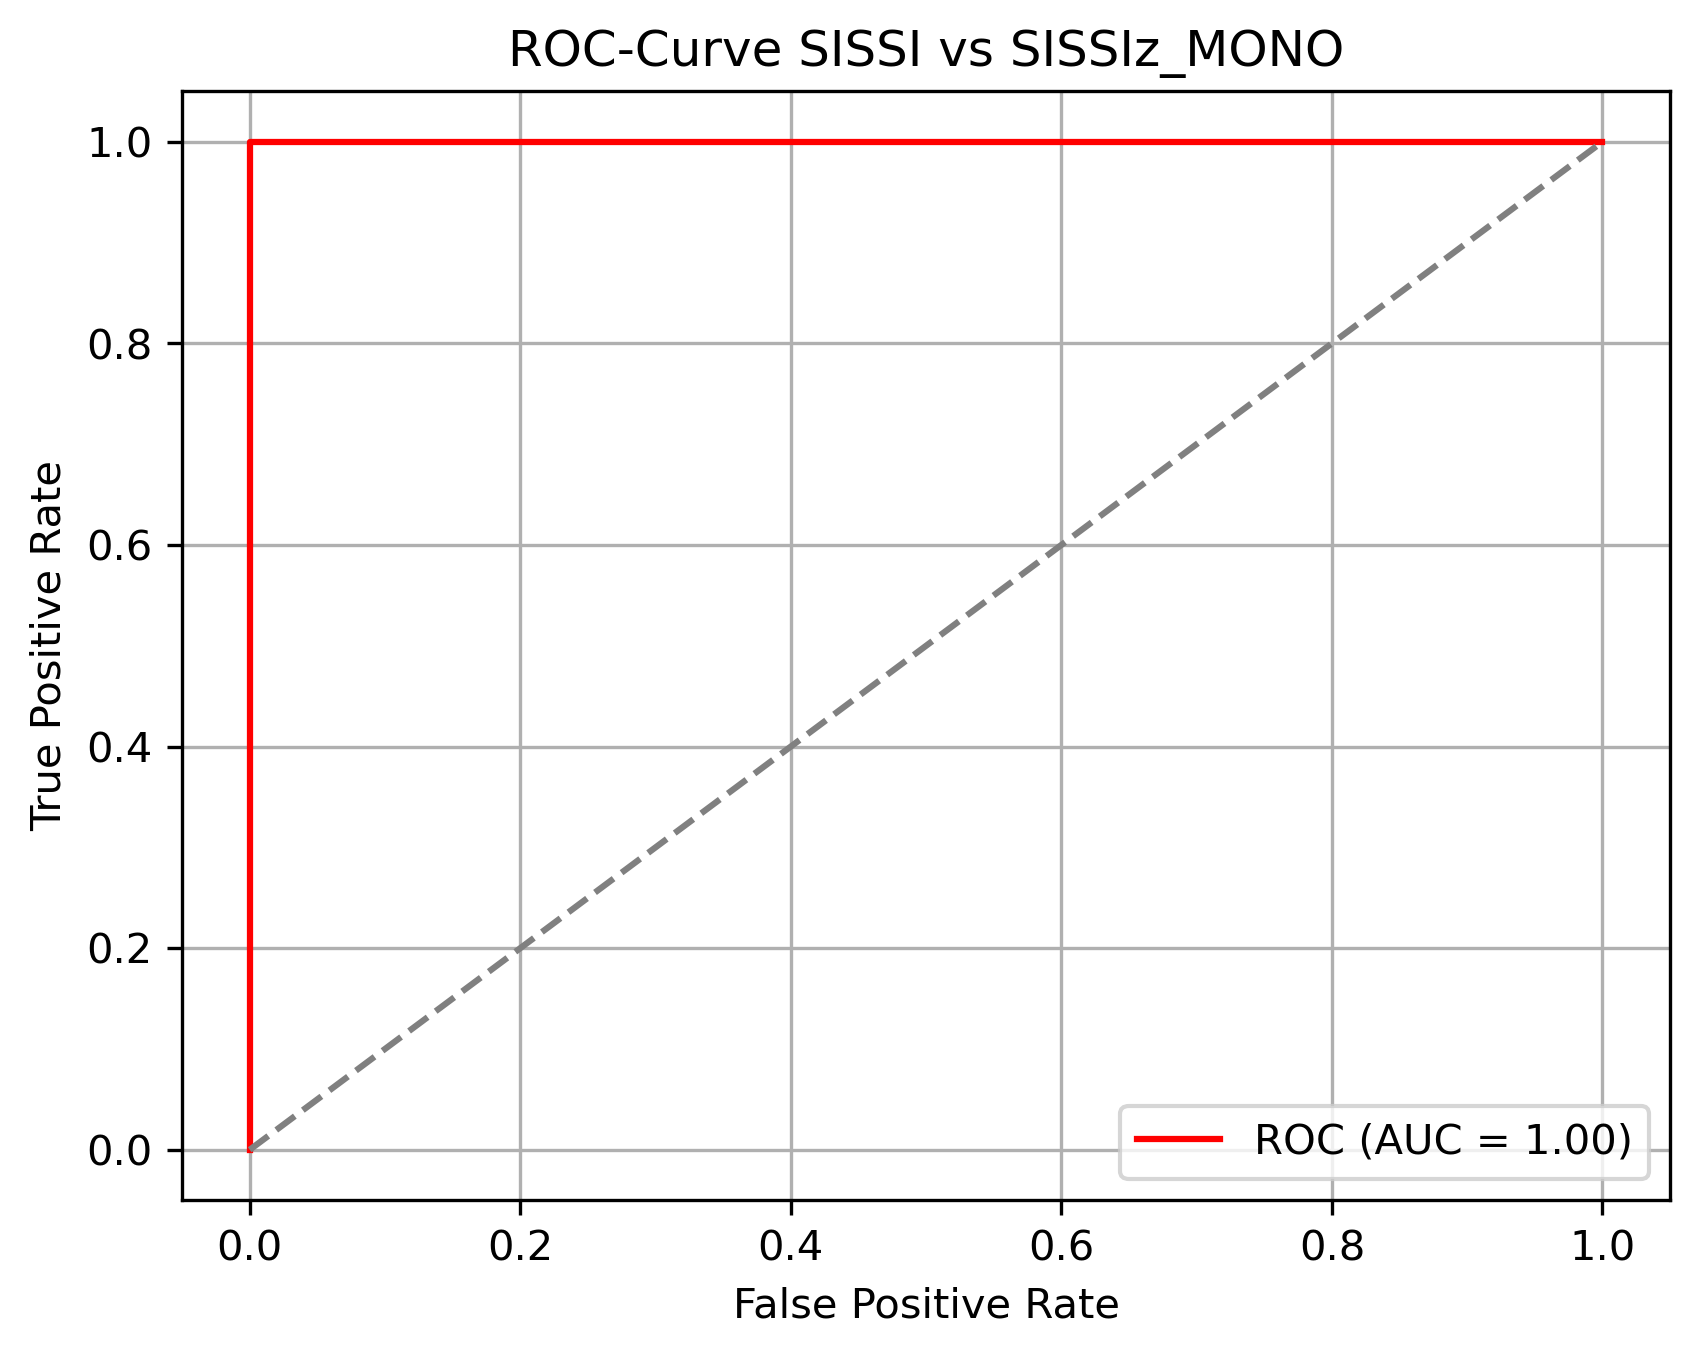
\includegraphics[width=\textwidth]{SISSIz_ROC_Curve_SISSI_vs_SISSIz_MONO.png}
        \caption{SISSI vs SISSIz-mono}
        \label{fig:roc_sissiz_mono}
    \end{subfigure}
    \hfill
    \begin{subfigure}[b]{0.48\textwidth}
        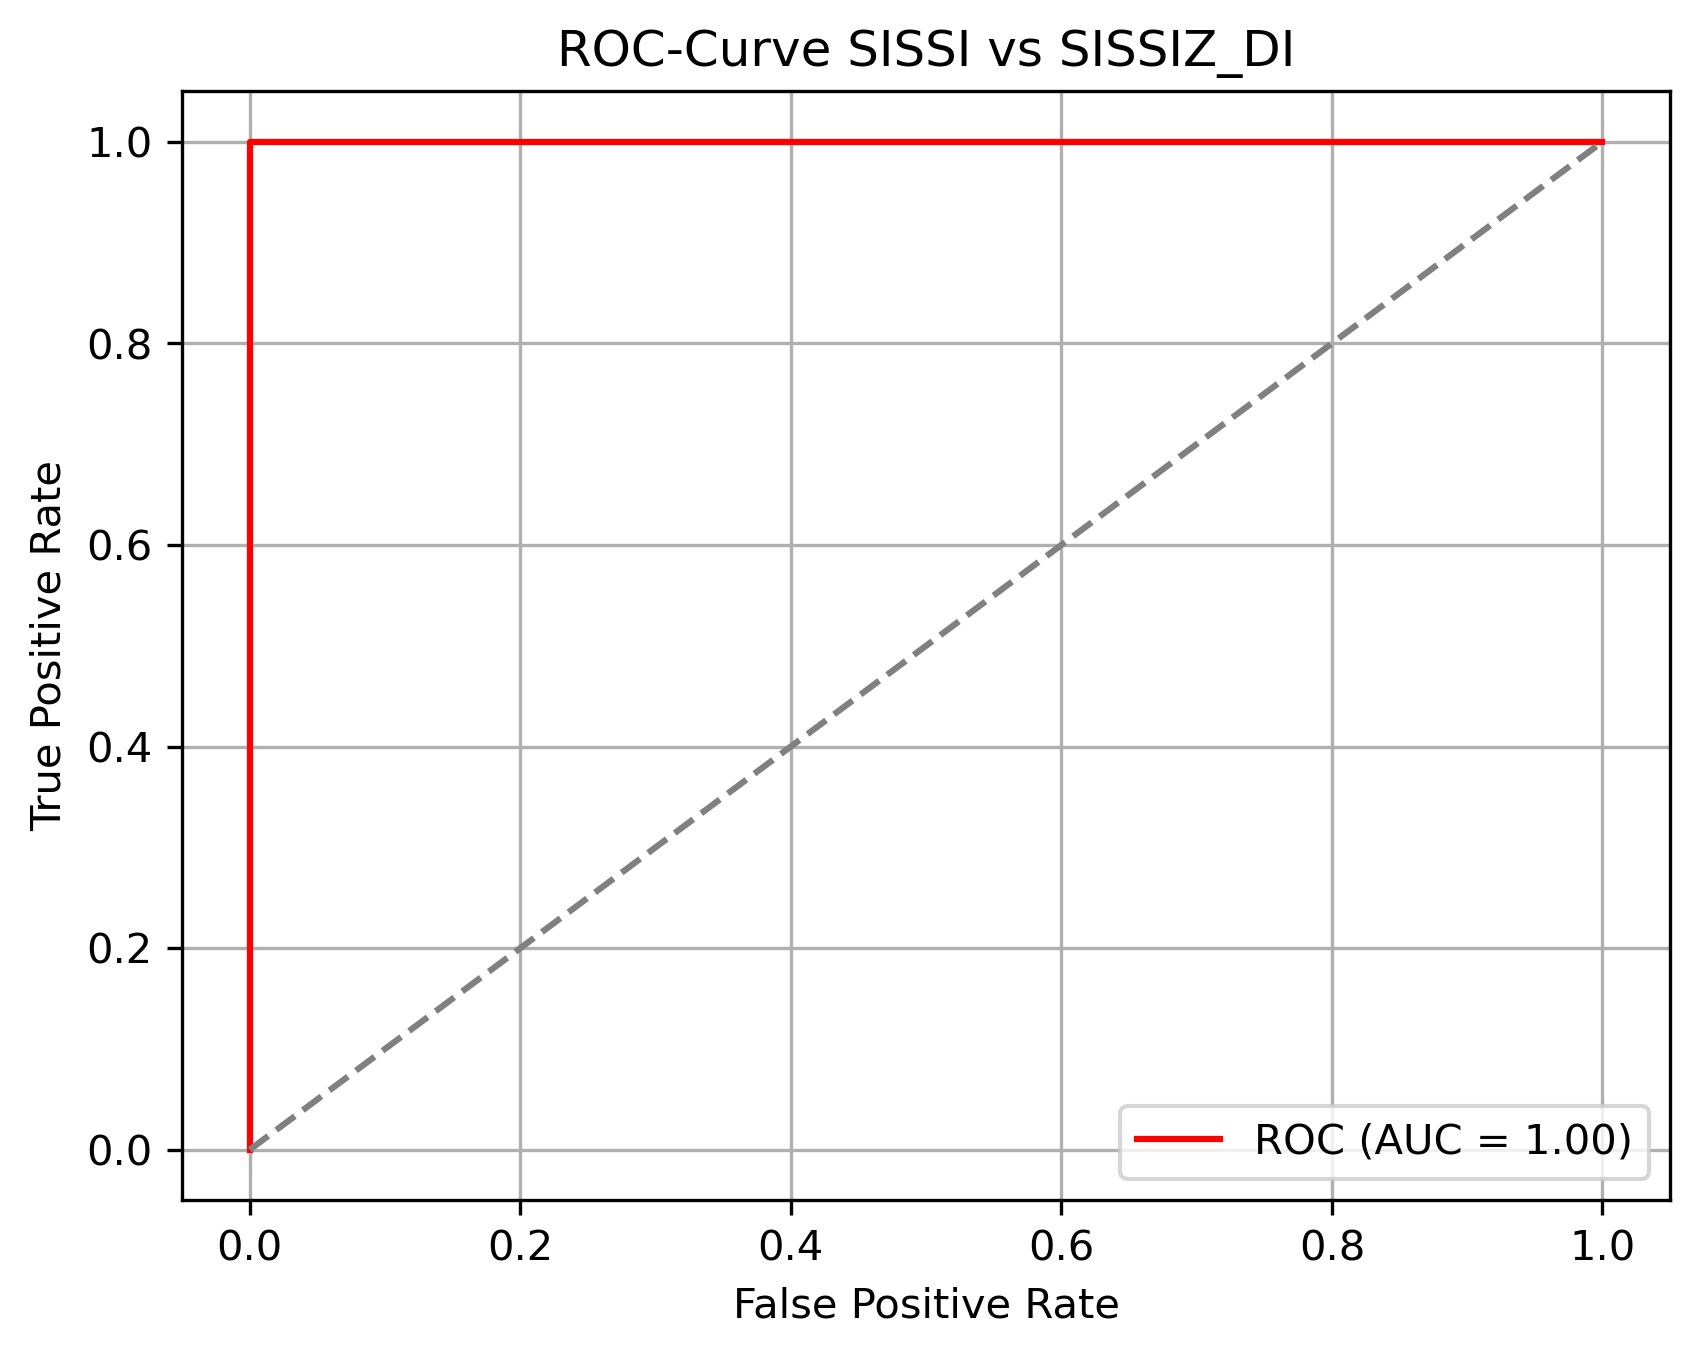
\includegraphics[width=\textwidth]{SISSIz_ROC_Curve_SISSI_vs_SISSIZ_DI.png}
        \caption{SISSI vs SISSIz-di}
        \label{fig:roc_sissiz_di}
    \end{subfigure}
    \vspace{1em}

    \begin{subfigure}[b]{0.48\textwidth}
        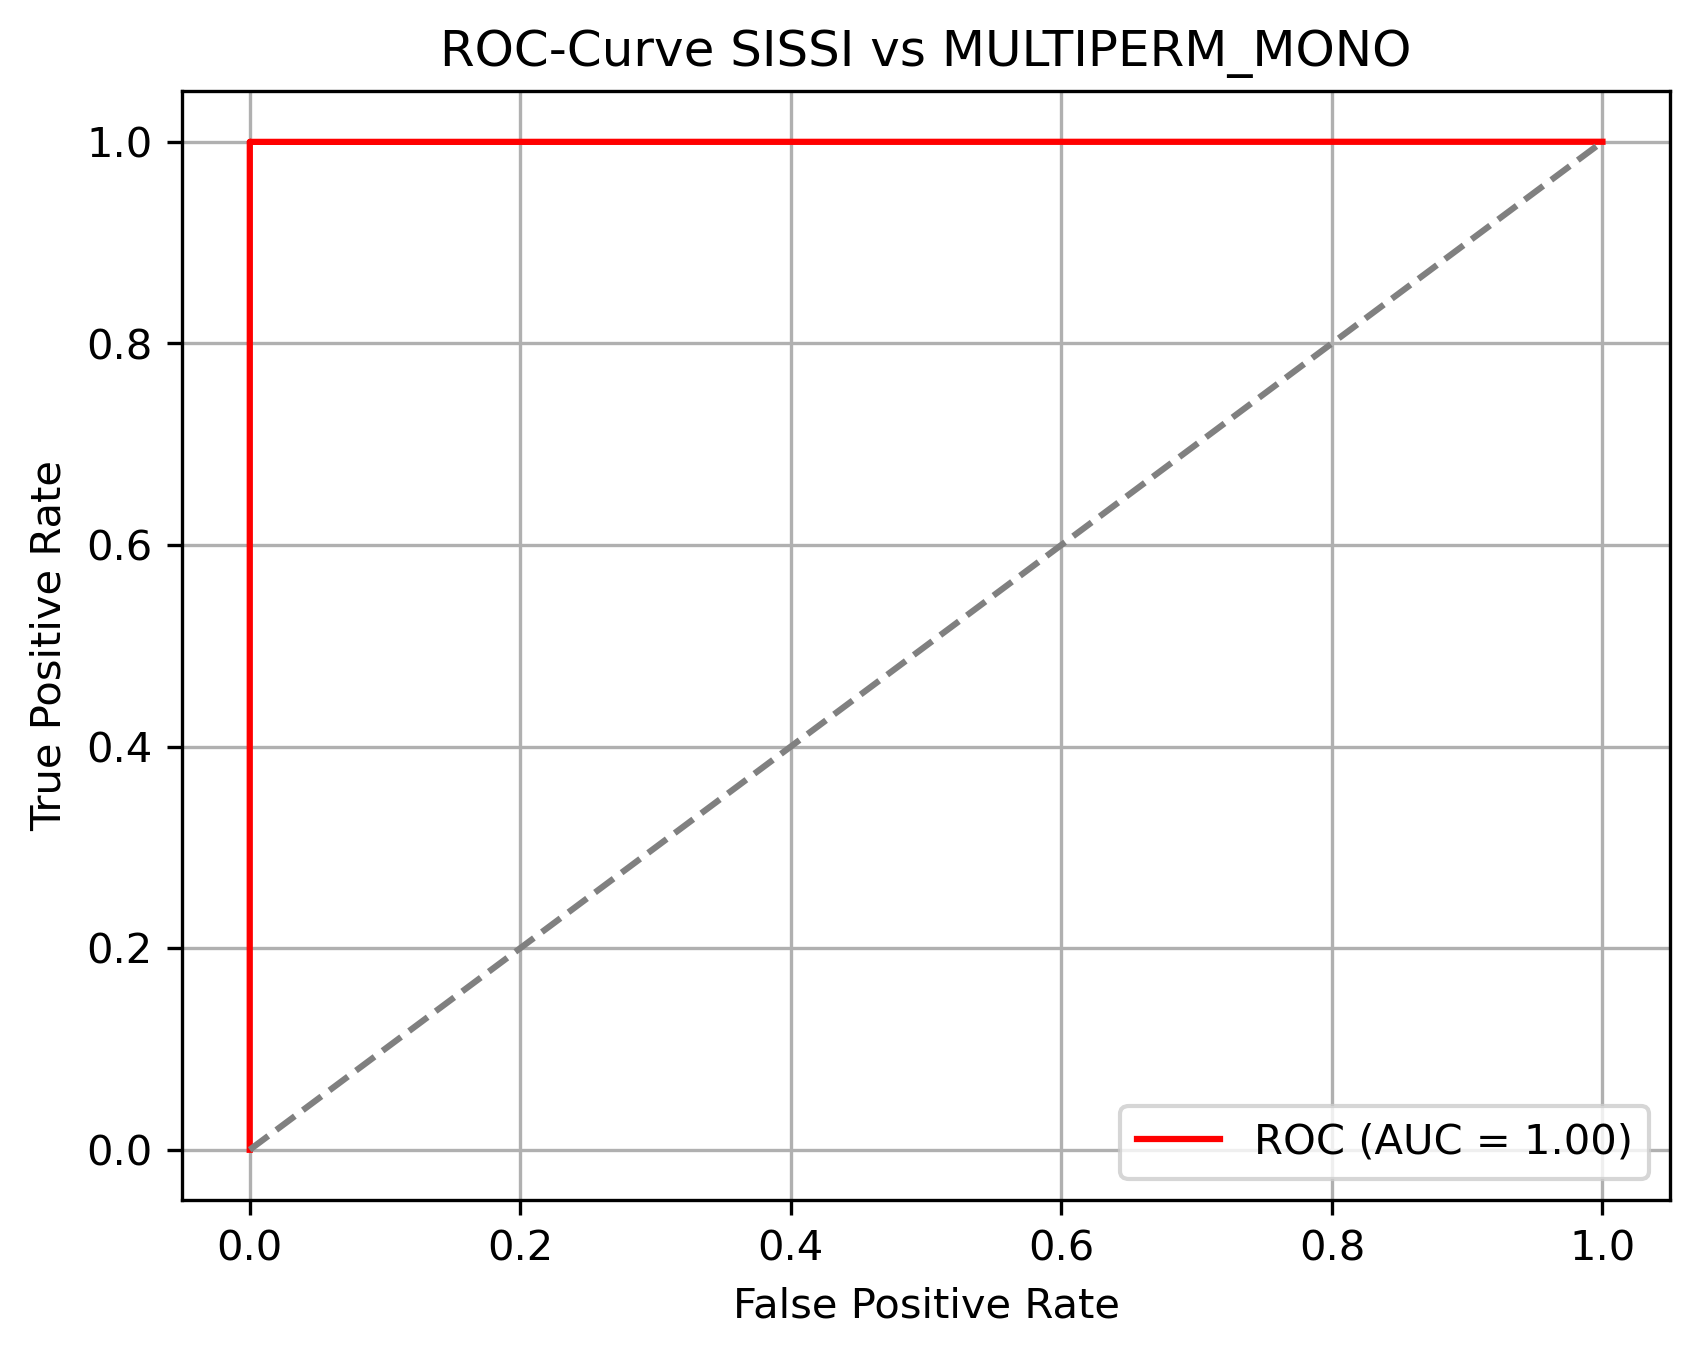
\includegraphics[width=\textwidth]{SISSIz_ROC_Curve_SISSI_vs_MULTIPERM_MONO.png}
        \caption{SISSI vs MULTIPERM-mono}
        \label{fig:roc_multiperm_mono}
    \end{subfigure}
    \hfill
    \begin{subfigure}[b]{0.48\textwidth}
        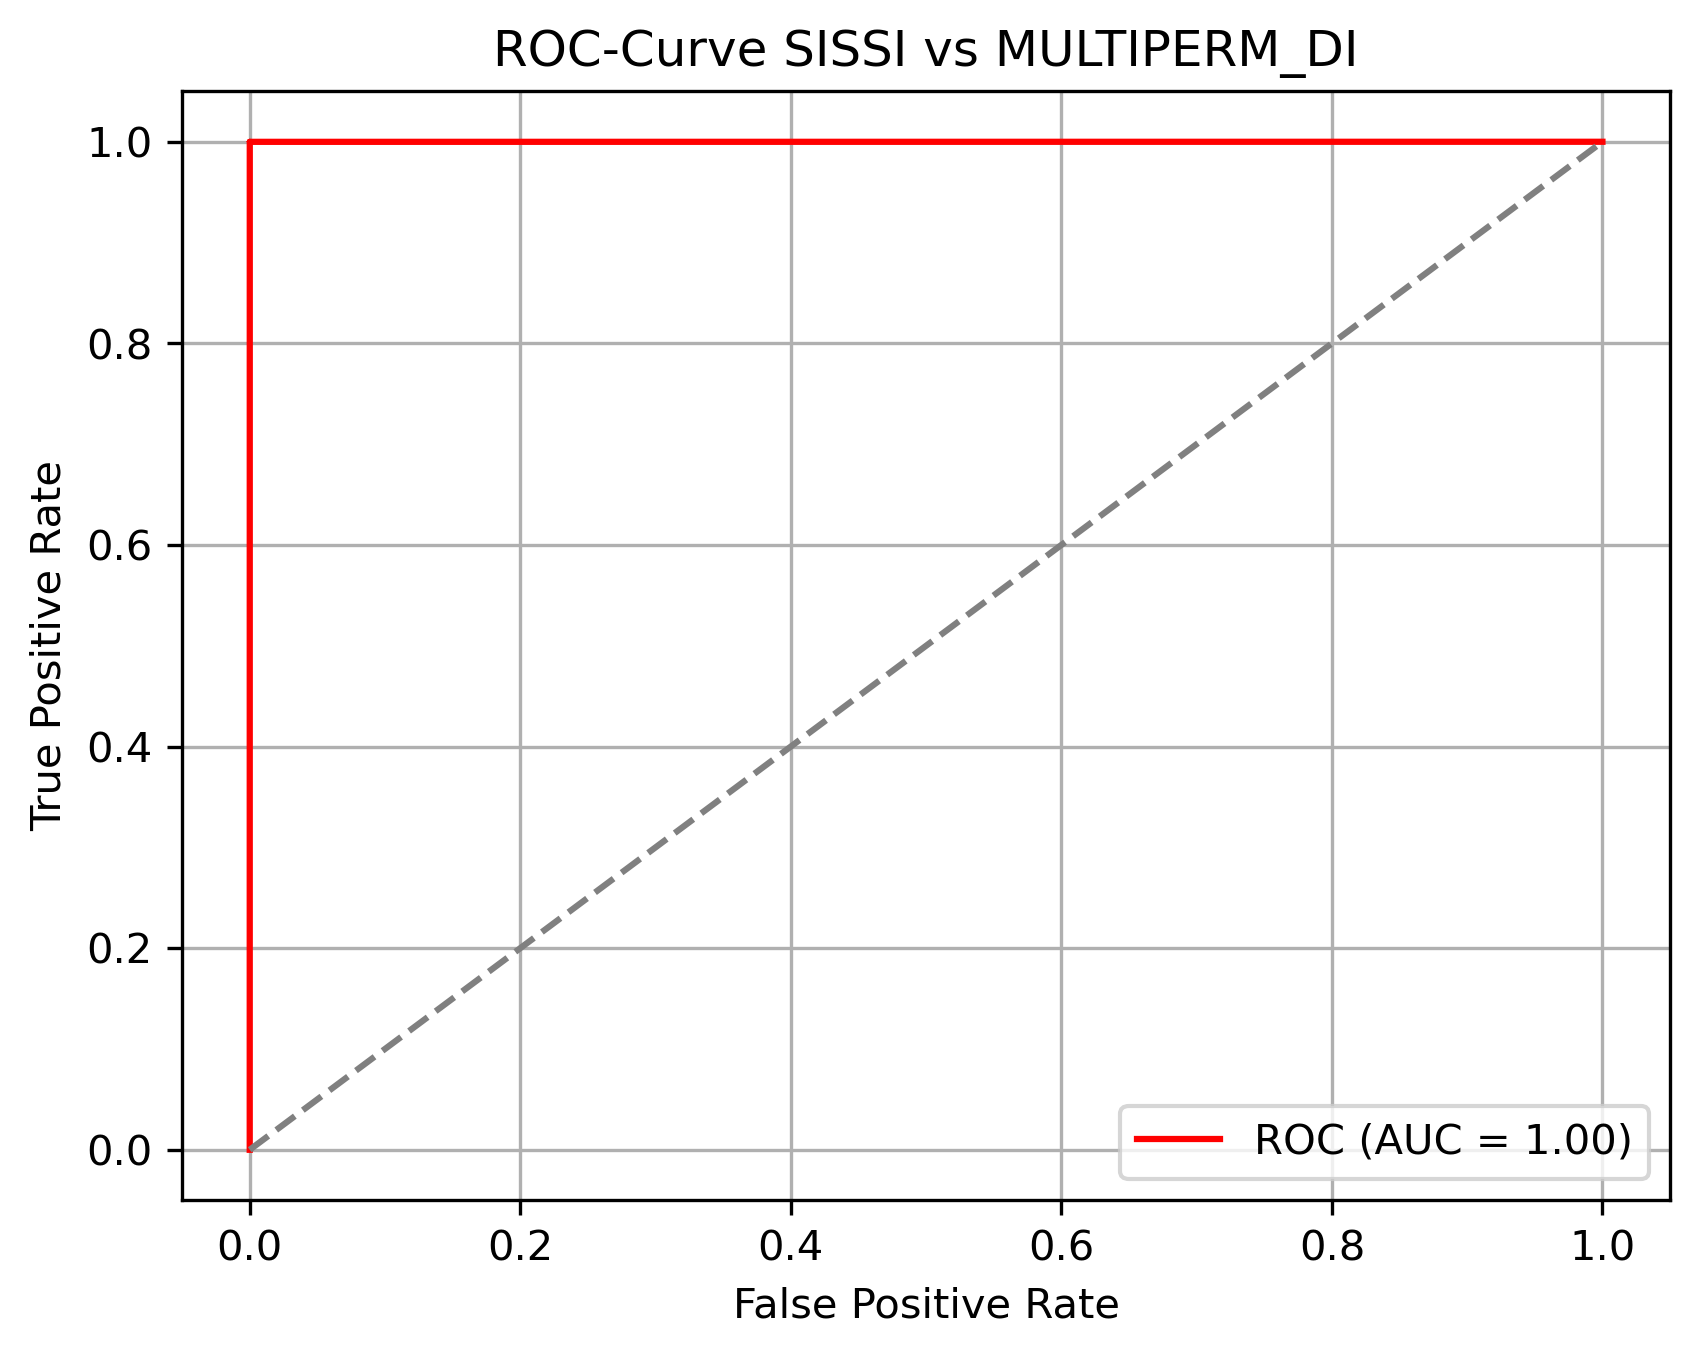
\includegraphics[width=\textwidth]{SISSIz_ROC_Curve_SISSI_vs_MULTIPERM_DI.png}
        \caption{SISSI vs MULTIPERM-di}
        \label{fig:roc_multiperm_di}
    \end{subfigure}
    \vspace{1em}

    \begin{subfigure}[b]{0.48\textwidth}
        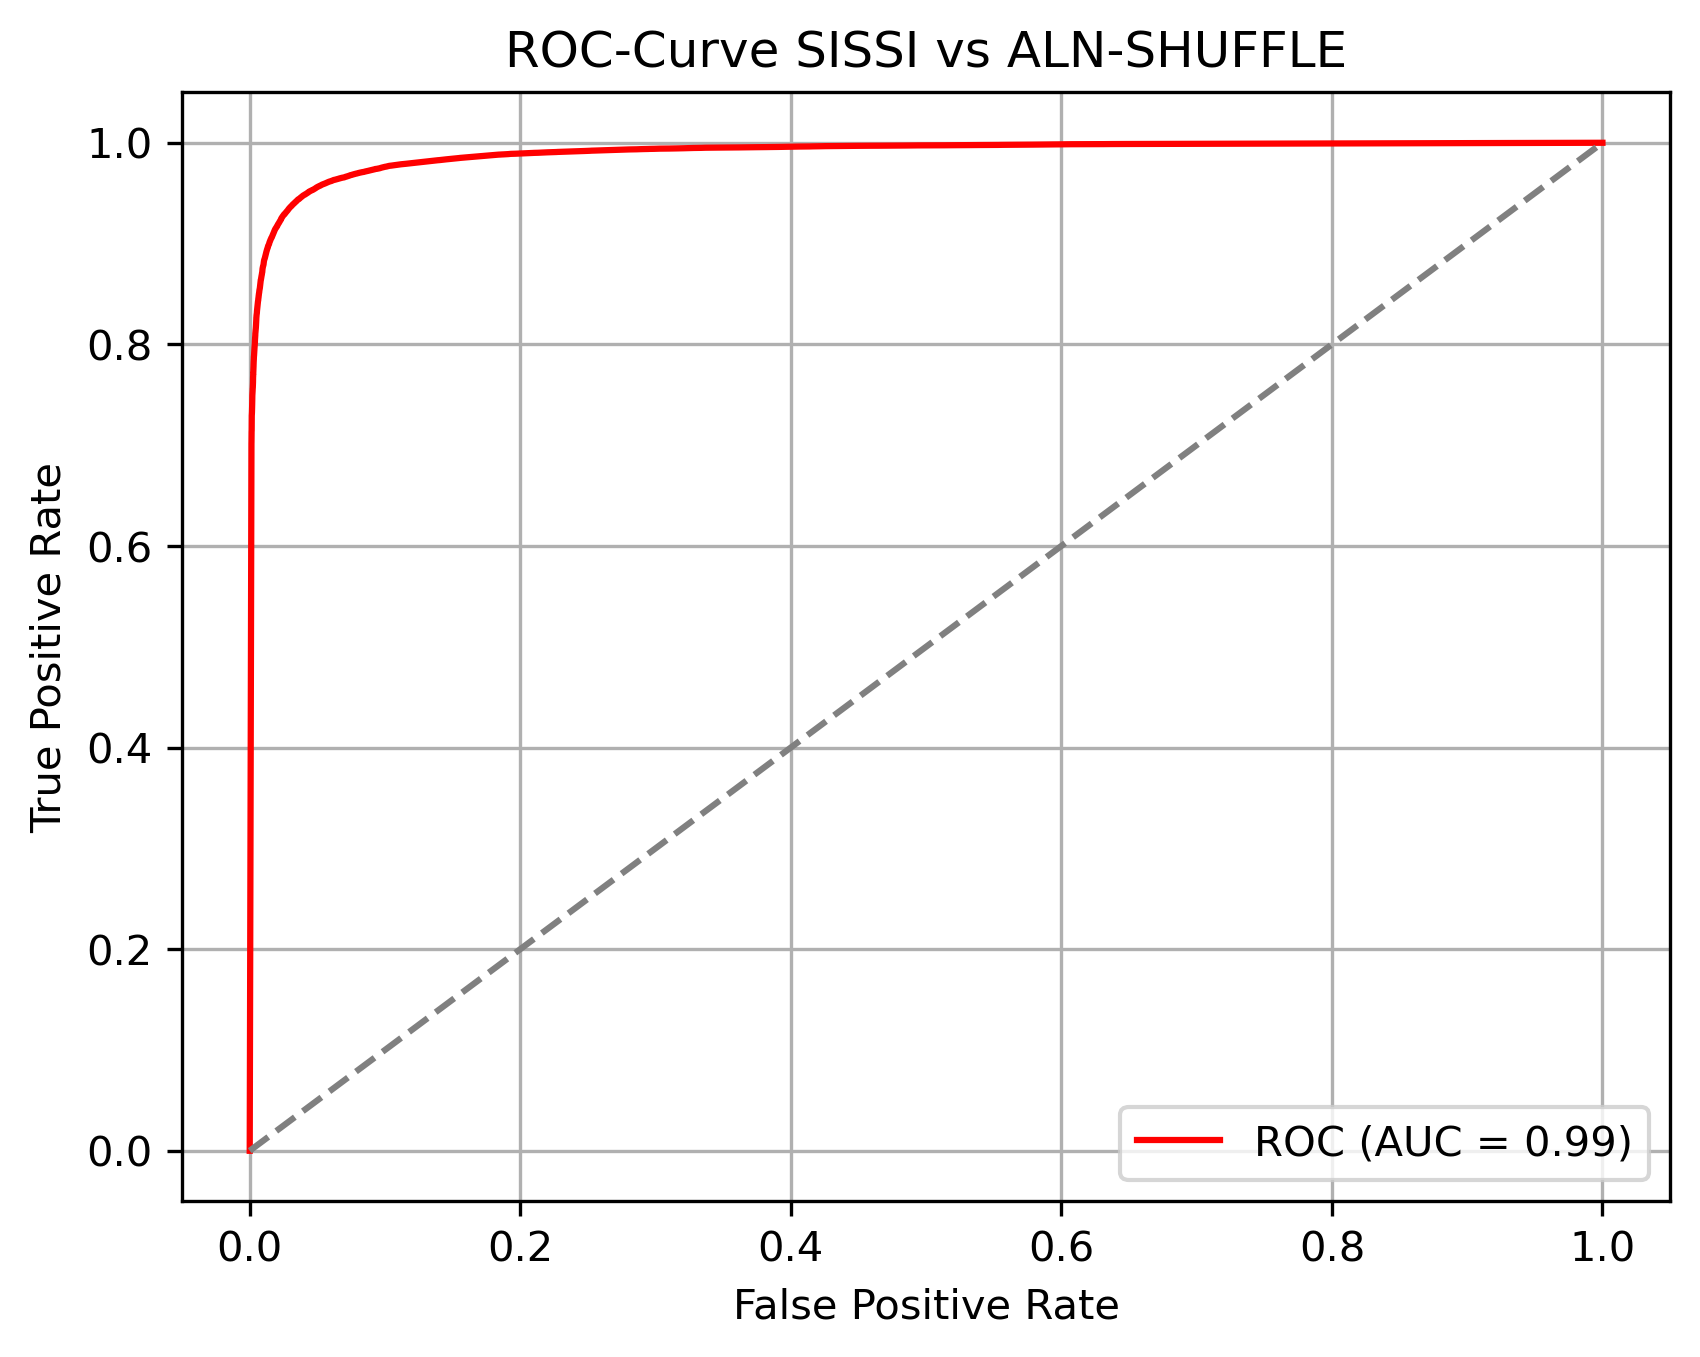
\includegraphics[width=\textwidth]{SISSIz_ROC_Curve_SISSI_vs_ALN-SHUFFLE.png}
        \caption{SISSI vs ALN-SHUFFLE}
        \label{fig:roc_aln_shuffle}
    \end{subfigure}

    \caption{ROC-curves from SISSIz prediction}
    \label{fig:all_roc_curves}
\end{figure}

The ROC curve compares the true-positive rate with the false-positive rate for various threshold values. The AUC value (Area Under the Curve) measures the quality of the separation between the classes.\vspace{1em}

The analysis of the classification performance showed that the SISSI model achieved excellent results in almost all comparison scenarios. Particularly striking was the AUC value in the Aln-Shuffle scenario, which was exceptionally high at 0{,}99 - despite the overall poorer separability in this case.\vspace{1em}

SISSIz-mono and SISSIz-di also showed very high AUC values, confirming their strong discriminatory power. The multiperm variants were slightly lower, but also showed useful classification results. In comparison, the Aln-Shuffle model presented the greatest challenge and, with an AUC of 0{,}95, achieved the lowest value of all the methods tested.\vspace{1em}

\clearpage

\section{Results of MXfold2 Prediction}

\subsection{RNA secondary structure prediction using deep learning with thermodynamic integration\href{https://doi.org/10.1038/s41467-021-21194-4   }{\textbf{[1]}}\href{https://github.com/mxfold/mxfold2?tab=readme-ov-file}{\textbf{[2]}}}

\subsection{MXfold2 Boxplot}
\begin{figure}[H]
    \centering
    \includegraphics[scale=0.7]{Boxplot Mxfold2 Score.png}
    \caption{Boxplot MXfold2 Score}
    \label{fig:bar_chart}
\end{figure}

The boxplot of MXfold2 clearly shows that the RNA secondary structure was successfully destroyed. However, MXfold2 shows difficulties in handling the simulated data from SISSI, which leads to an inaccurate prediction of whether the secondary structure was actually destroyed or not. This observation could also explain why the Multiperm-mono and Multiperm-di methods achieve almost equivalent results to SISSIz-mono and SISSIz-di, although the evaluations of RNAz and SISSIz consistently show that the SISSIz-mono and SISSIz-di methods generally perform better than the other approaches.

\subsection{MXfold2 Histograms}

\begin{figure}[H]
    \centering
    \begin{subfigure}[b]{0.48\textwidth}
        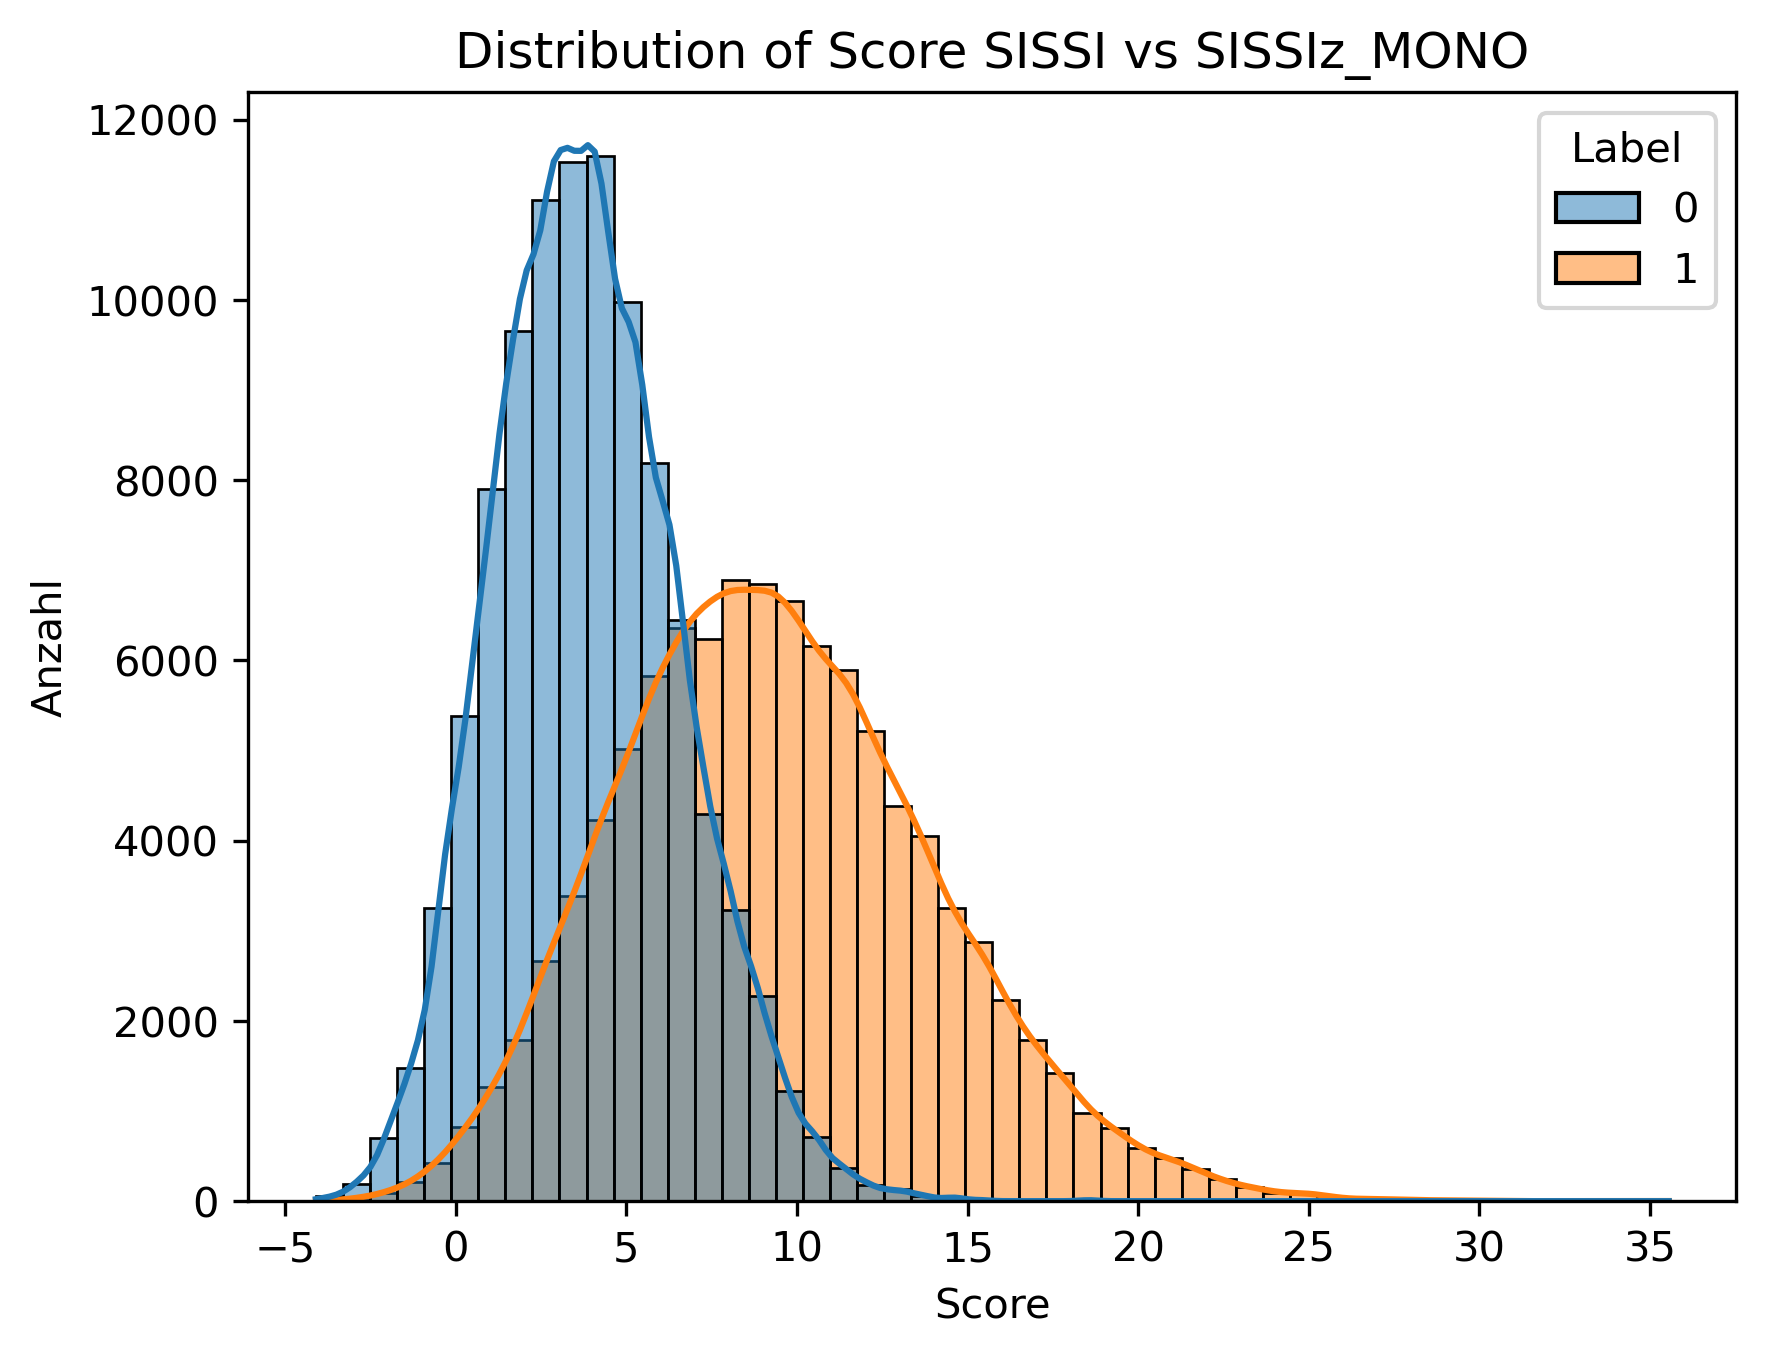
\includegraphics[width=\textwidth]{MXfold2_Histogram_SISSI_vs_SISSIz_MONO.png}
        \caption{SISSI vs SISSIz-mono}
        \label{fig:hist_sissiz_mono}
    \end{subfigure}
    \hfill
    \begin{subfigure}[b]{0.48\textwidth}
        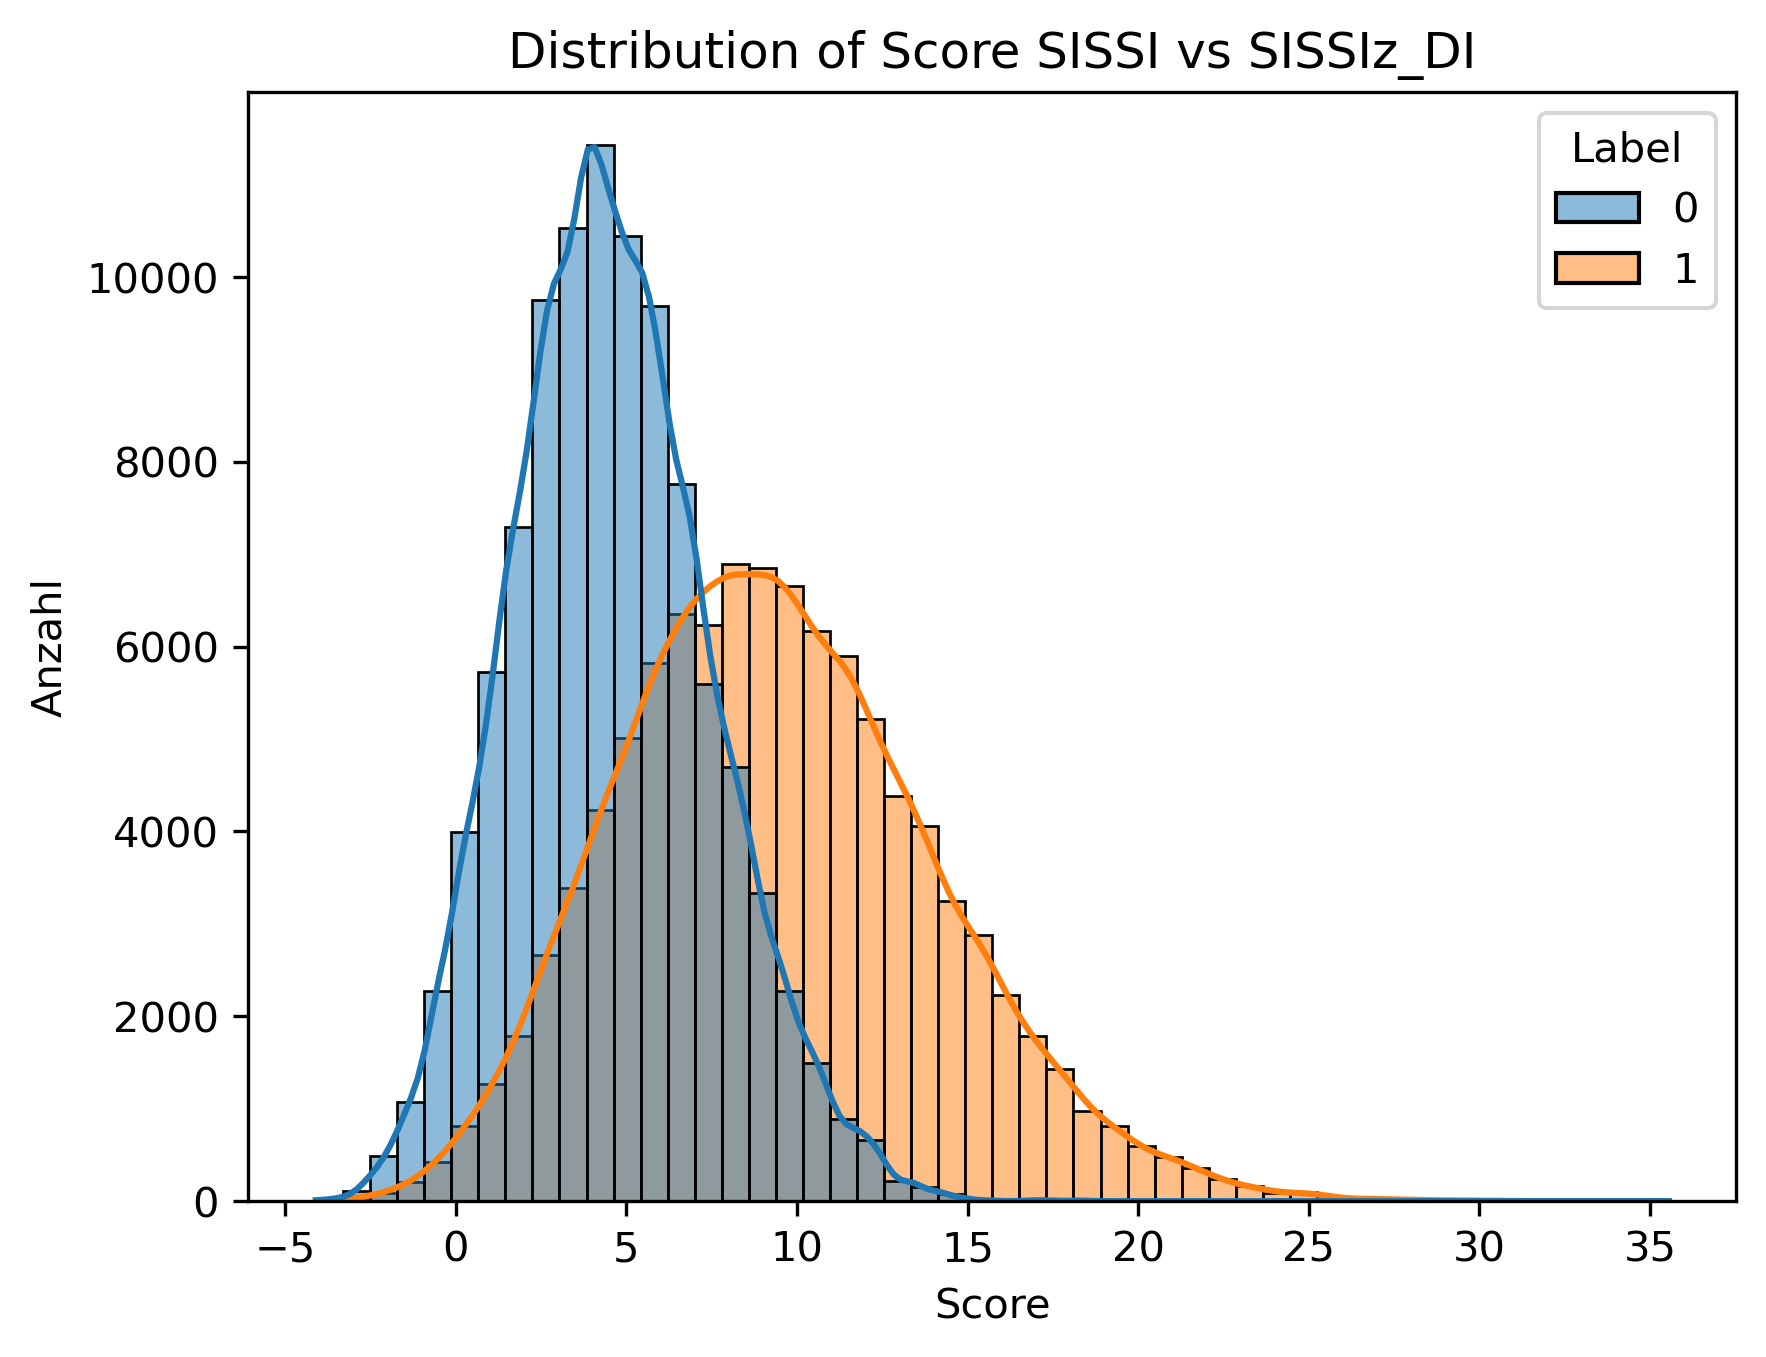
\includegraphics[width=\textwidth]{MXfold2_Histogram_SISSI_vs_SISSIz_DI.png}
        \caption{SISSI vs SISSIz-di}
        \label{fig:hist_sissiz_di}
    \end{subfigure}
    \vspace{1em}
    
    \begin{subfigure}[b]{0.48\textwidth}
        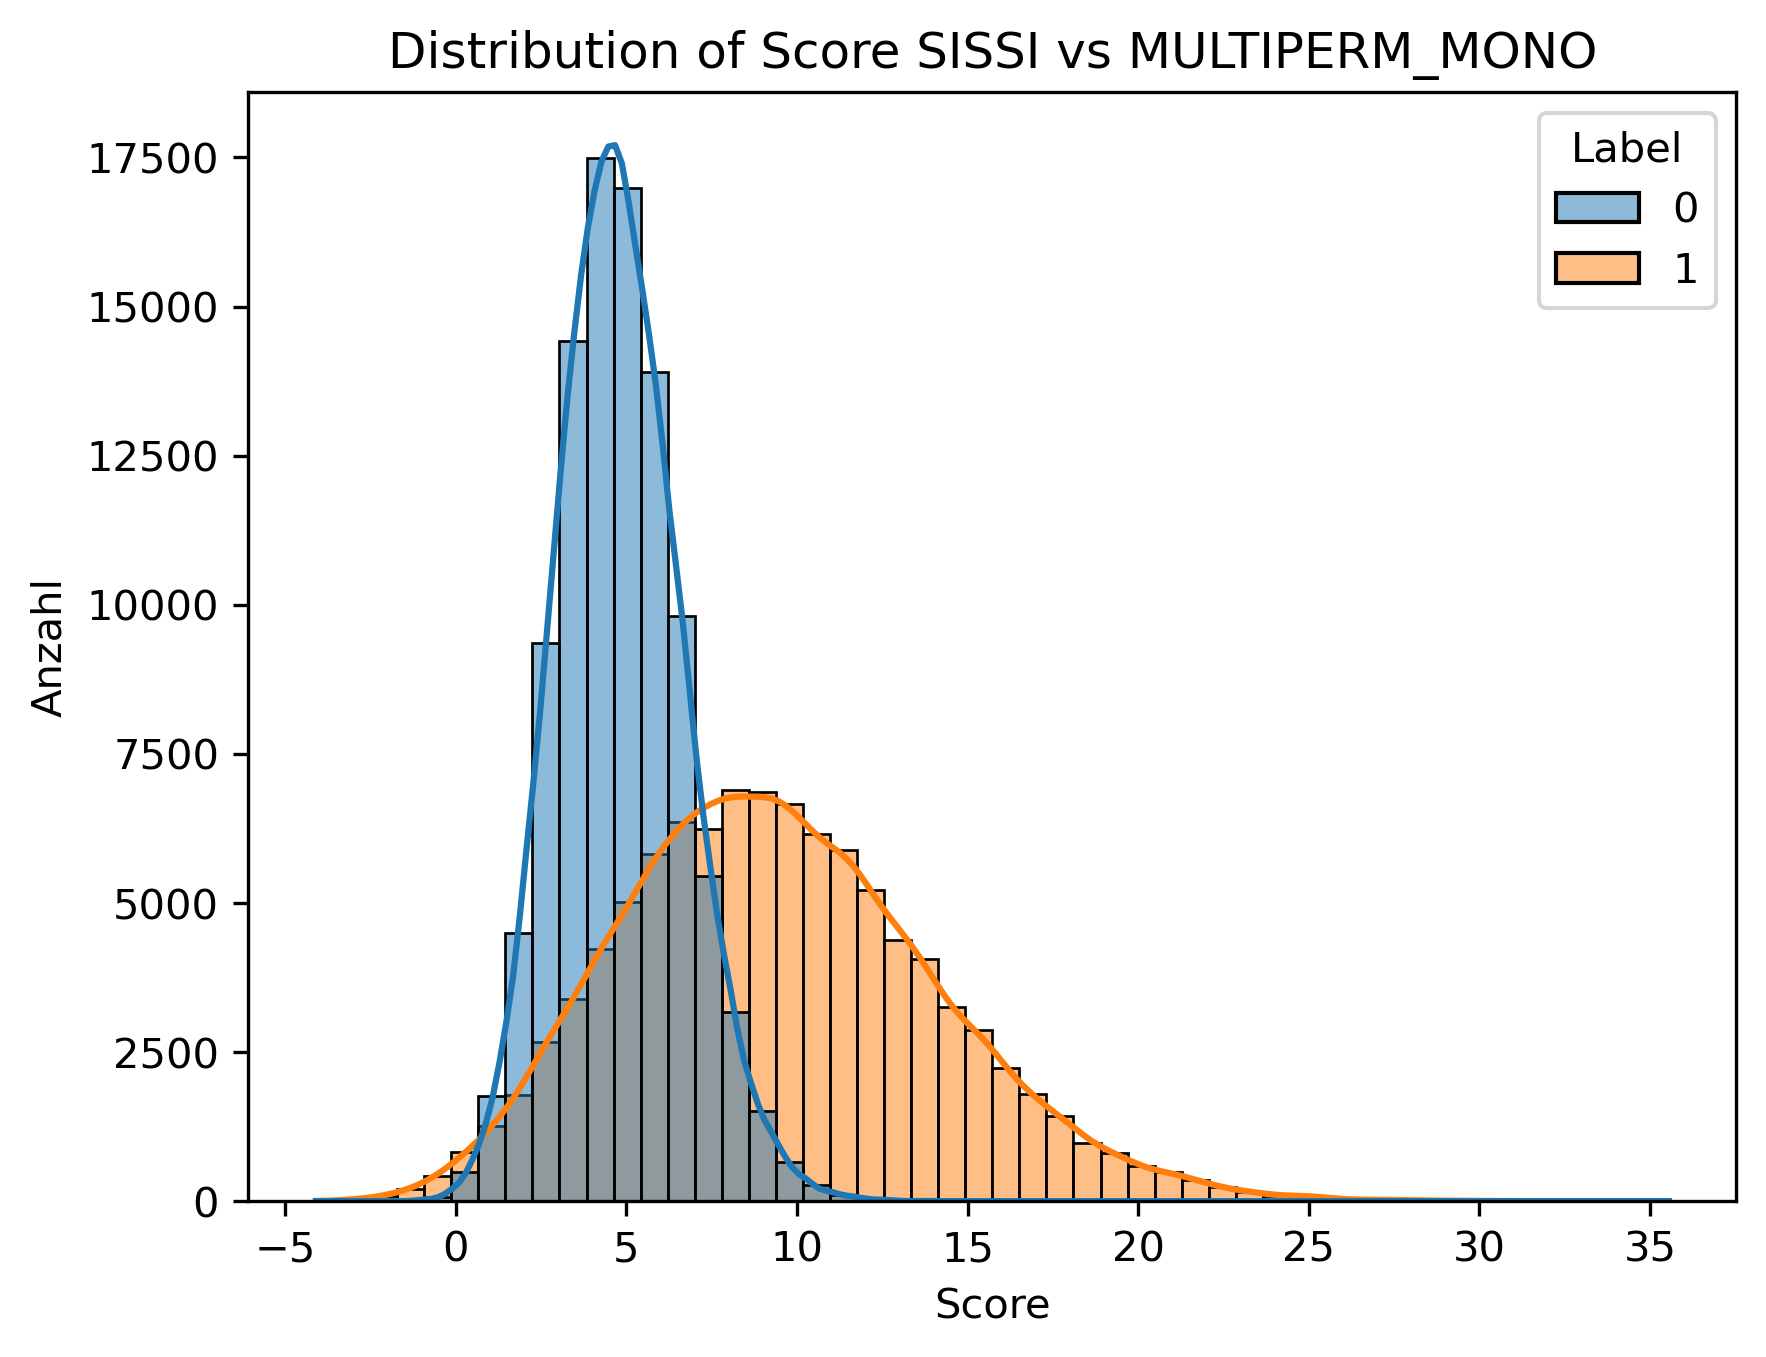
\includegraphics[width=\textwidth]{MXfold2_Histogram_SISSI_vs_MULTIPERM_MONO.png}
        \caption{SISSI vs MULTIPERM-mono}
        \label{fig:hist_multiperm_mono}
    \end{subfigure}
    \hfill
    \begin{subfigure}[b]{0.48\textwidth}
        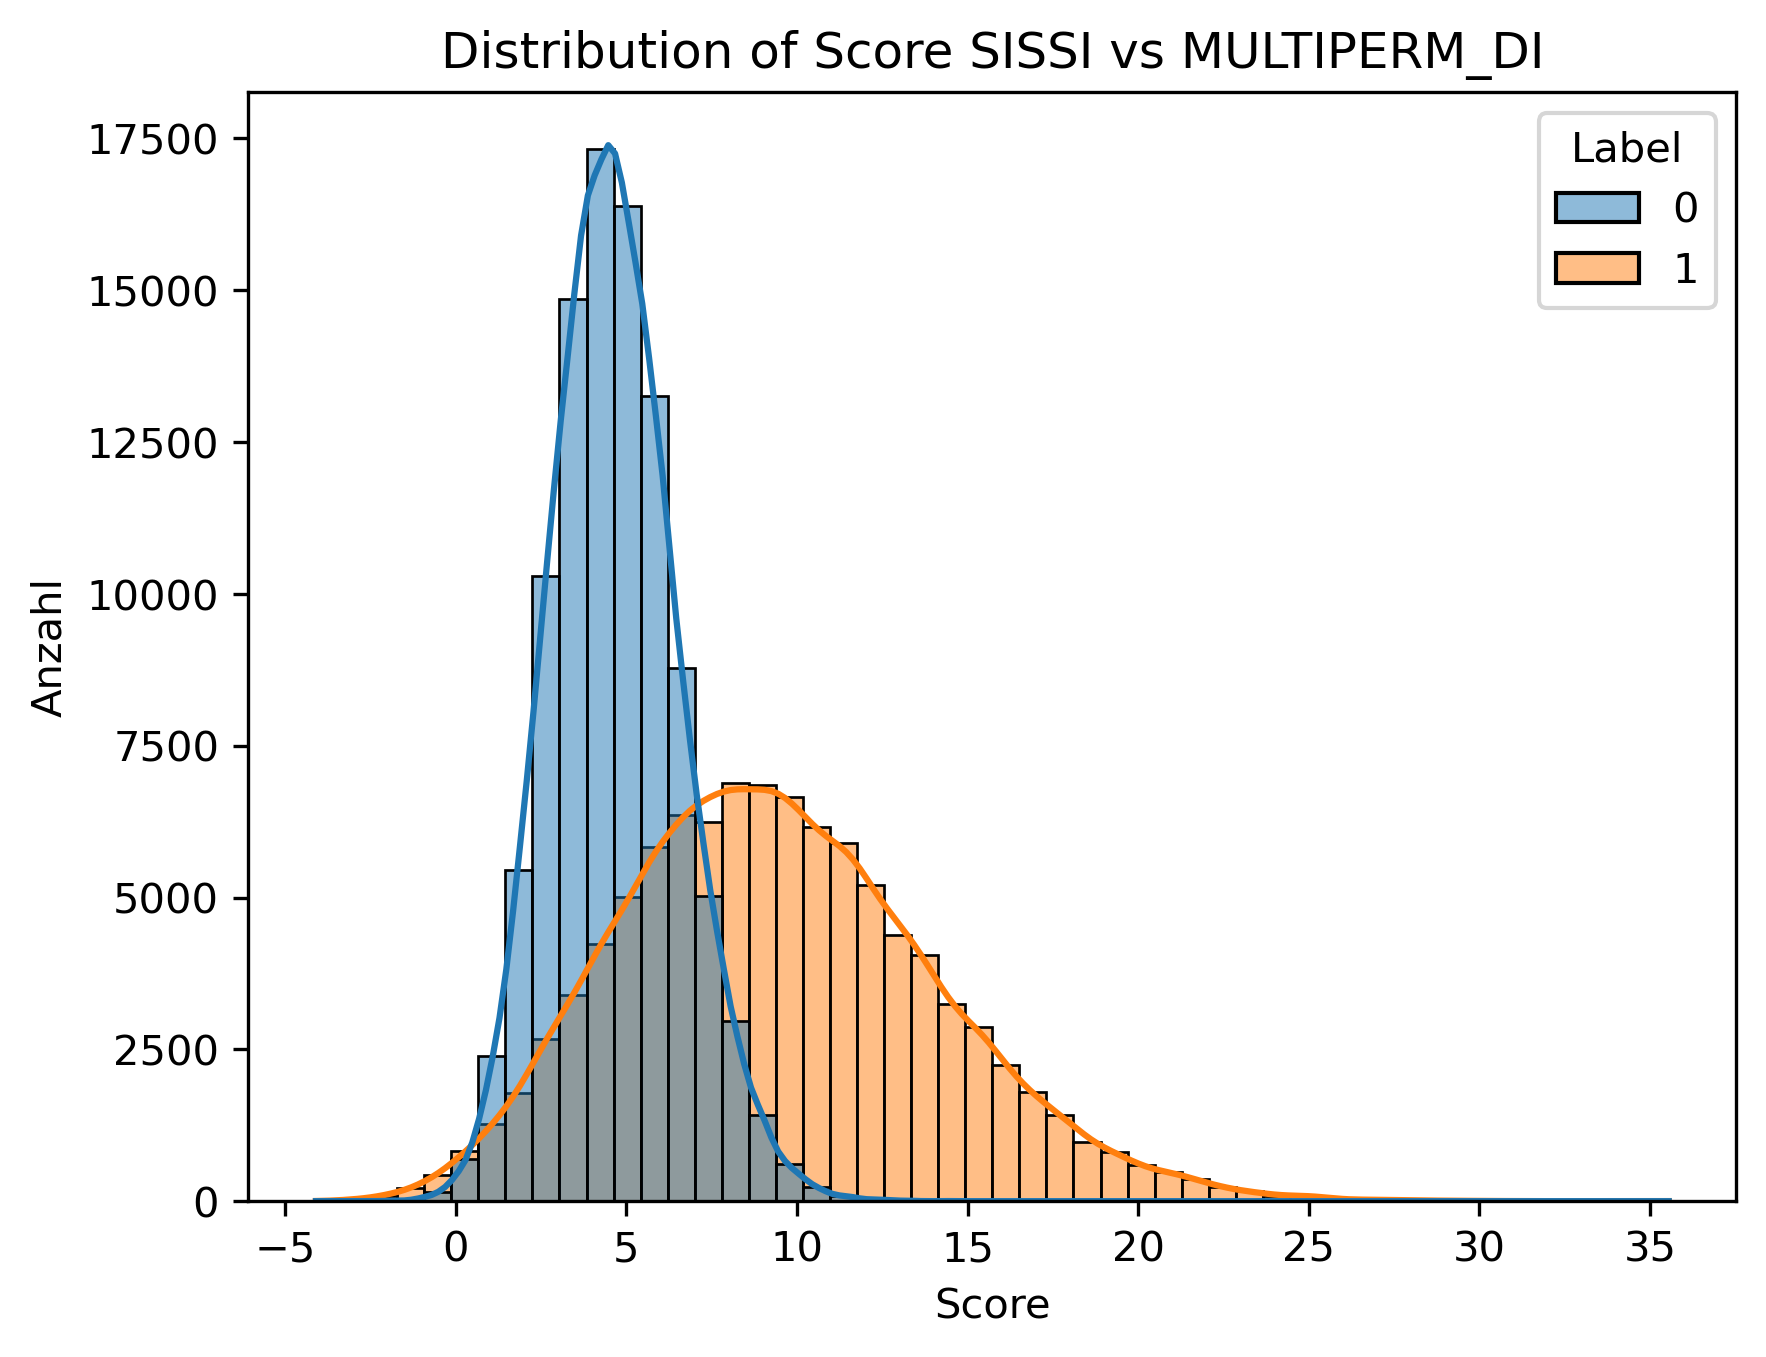
\includegraphics[width=\textwidth]{MXfold2_Histogram_SISSI_vs_MULTIPERM_DI.png}
        \caption{SISSI vs MULTIPERM-di}
        \label{fig:hist_multiperm_di}
    \end{subfigure}
    \vspace{1em}
    
    \begin{subfigure}[b]{0.48\textwidth}
        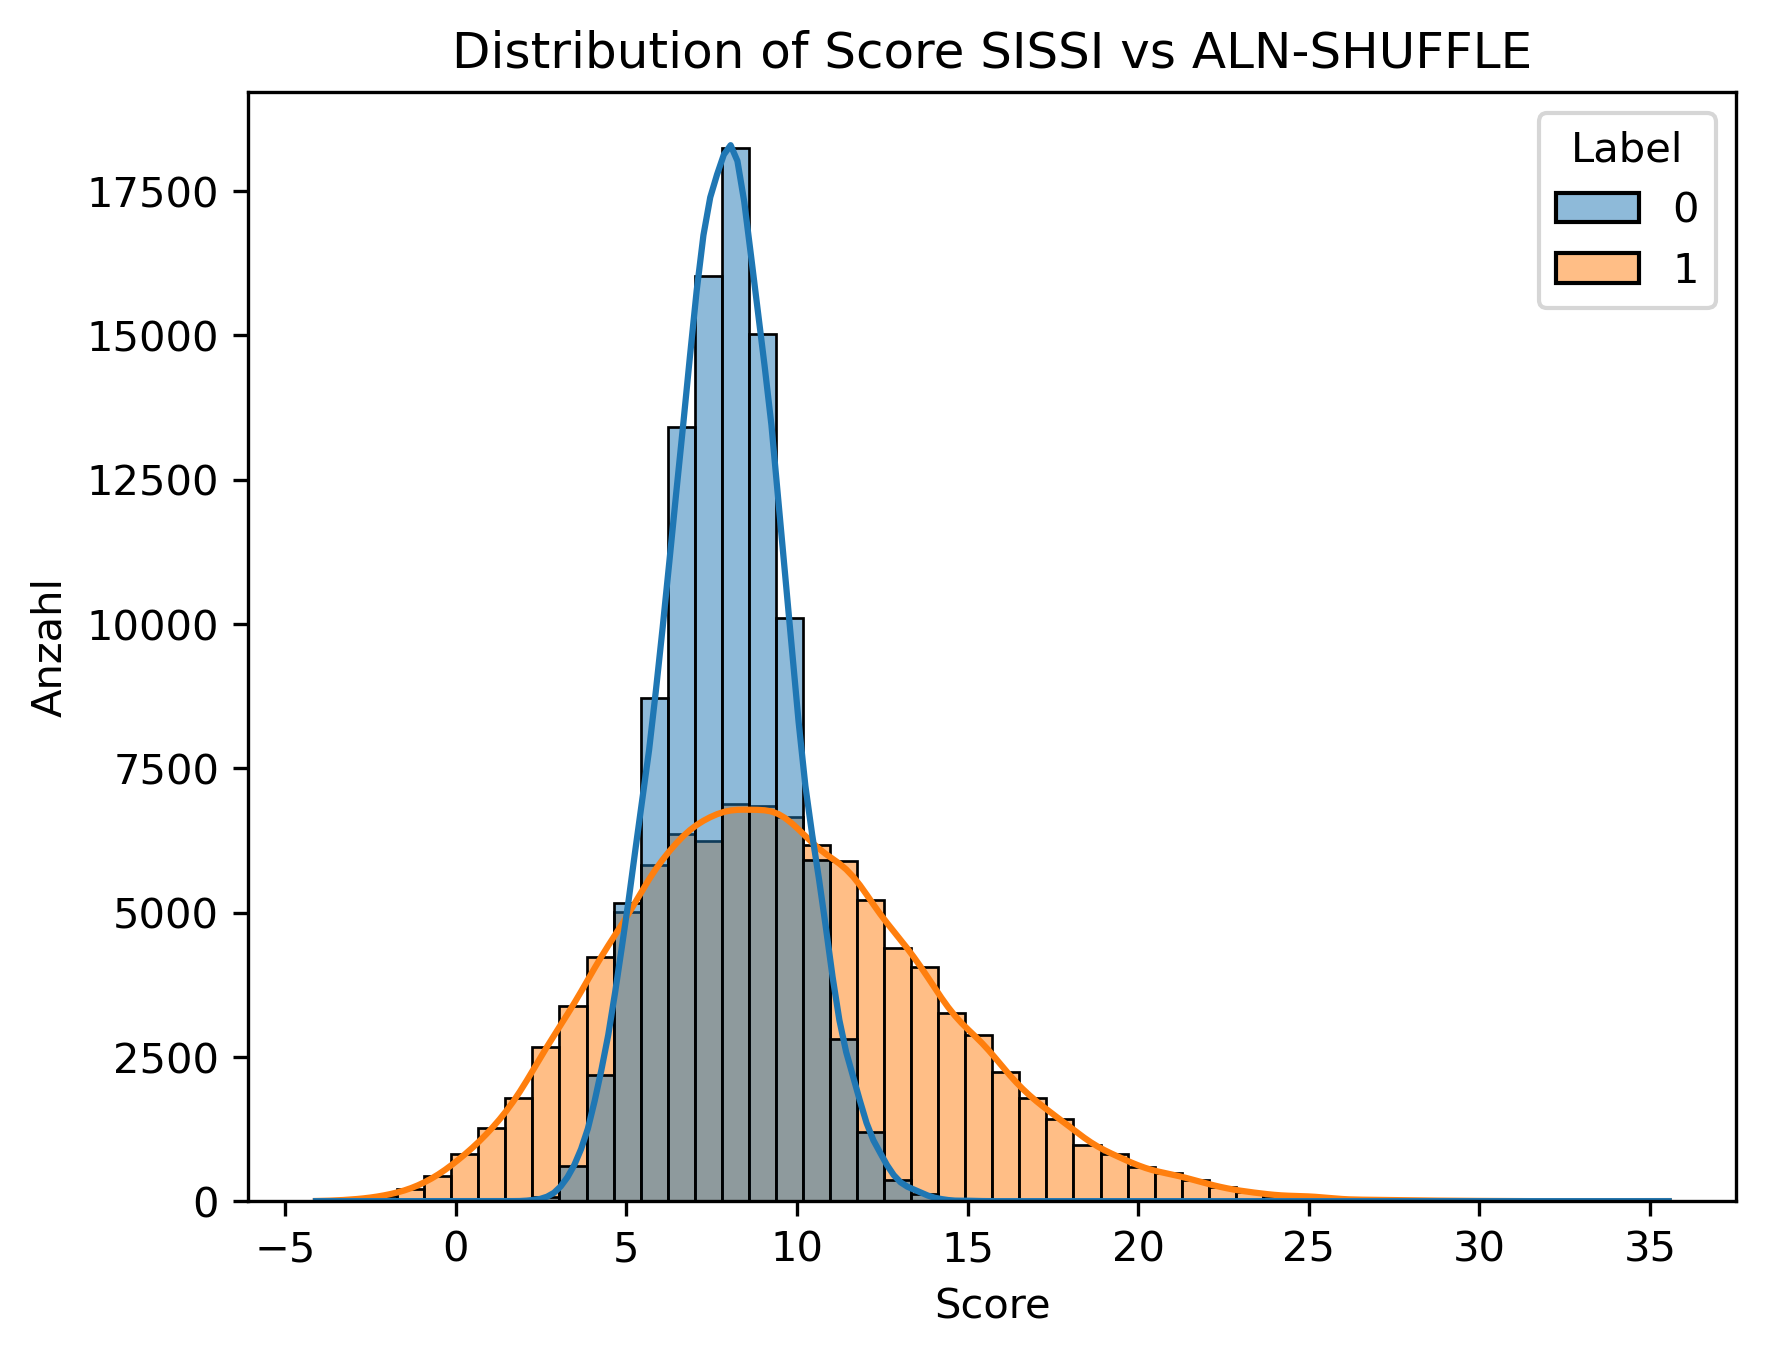
\includegraphics[width=\textwidth]{MXfold2_Histogram_SISSI_vs_ALN-SHUFFLE.png}
        \caption{SISSI vs ALN-SHUFFLE}
        \label{fig:hist_aln_shuffle}
    \end{subfigure}

    \caption{Histograms from MXfold2 prediction}
    \label{fig:all_histograms}
\end{figure}

When analyzing the histograms of the individual models, it becomes apparent that the positive and negative data are strongly intertwined. This indicates that the predictive accuracy of the random forest model may be limited. One possible explanation for this could be that all five histograms show almost identical results, which indicates that the MXfold2 model has difficulties in dealing with simulated data.

\subsection{MXfold2 Confusion Matrix}

\begin{figure}[H]
    \centering
    \begin{subfigure}[b]{0.48\textwidth}
        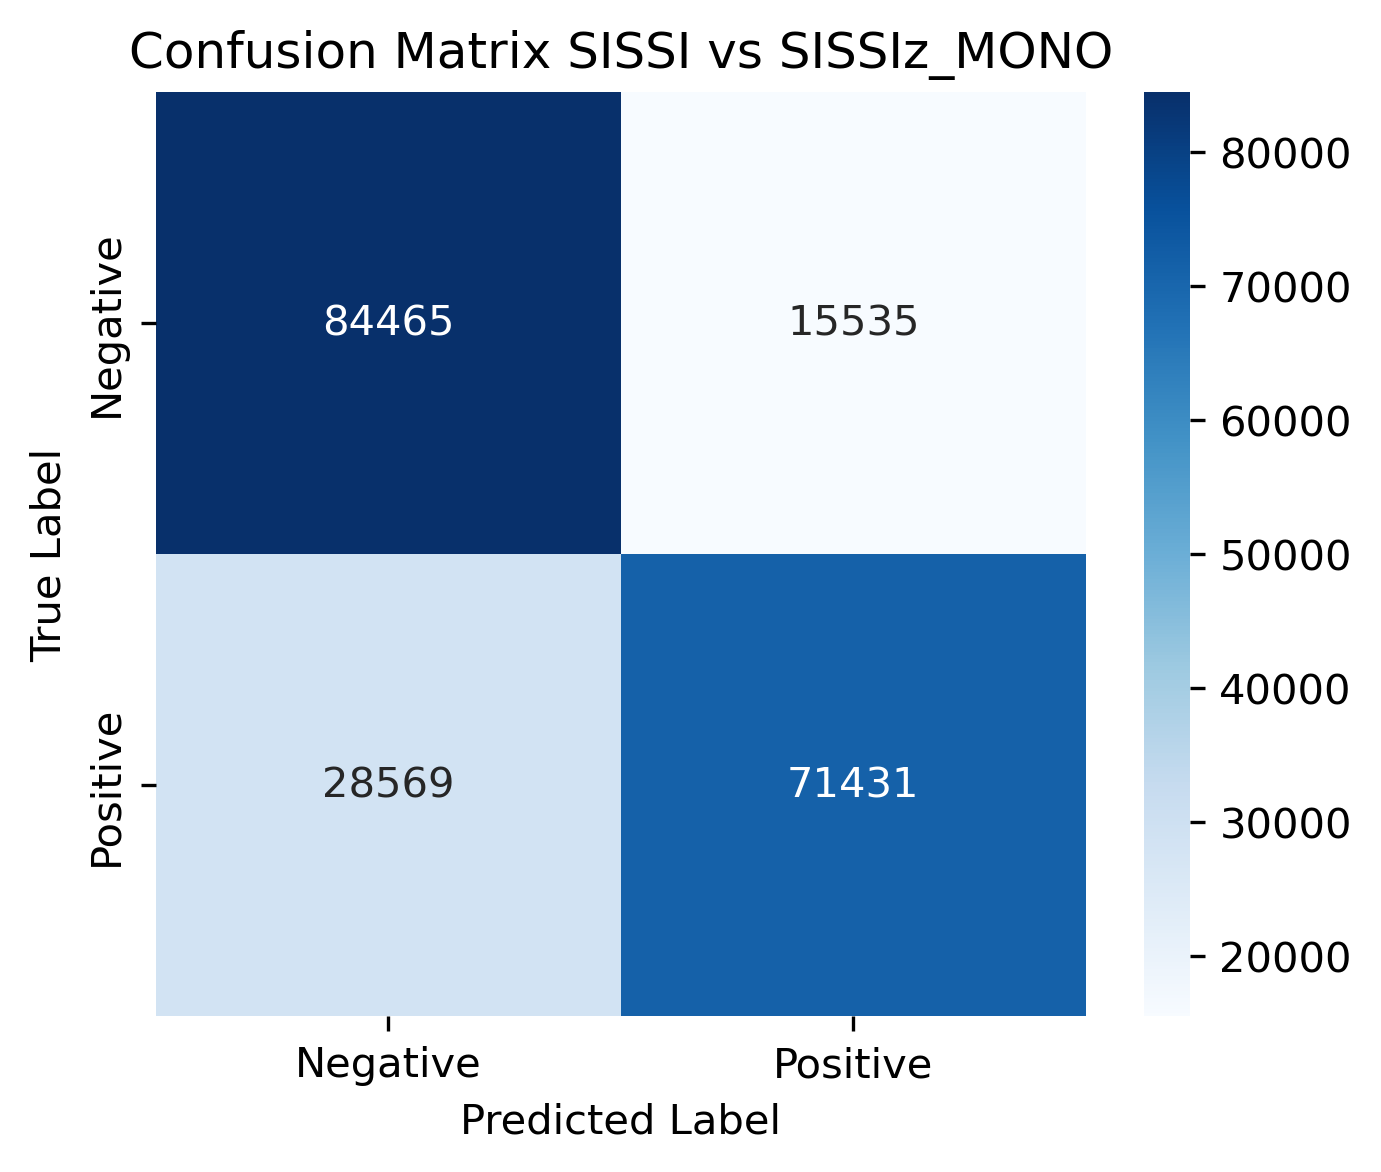
\includegraphics[width=\textwidth]{MXfold2_Confusion_Matrix_SISSI_vs_SISSIz_MONO.png}
        \caption{SISSI vs SISSIz-mono}
        \label{fig:confusion_sissiz_mono}
    \end{subfigure}
    \hfill
    \begin{subfigure}[b]{0.48\textwidth}
        \includegraphics[width=\textwidth]{MXfold2_Confusion_Matrix_SISSI_vs_SISSIZ_DI.png}
        \caption{SISSI vs SISSIz-di}
        \label{fig:confusion_sissiz_di}
    \end{subfigure}
    \vspace{1em}
    
    \begin{subfigure}[b]{0.48\textwidth}
        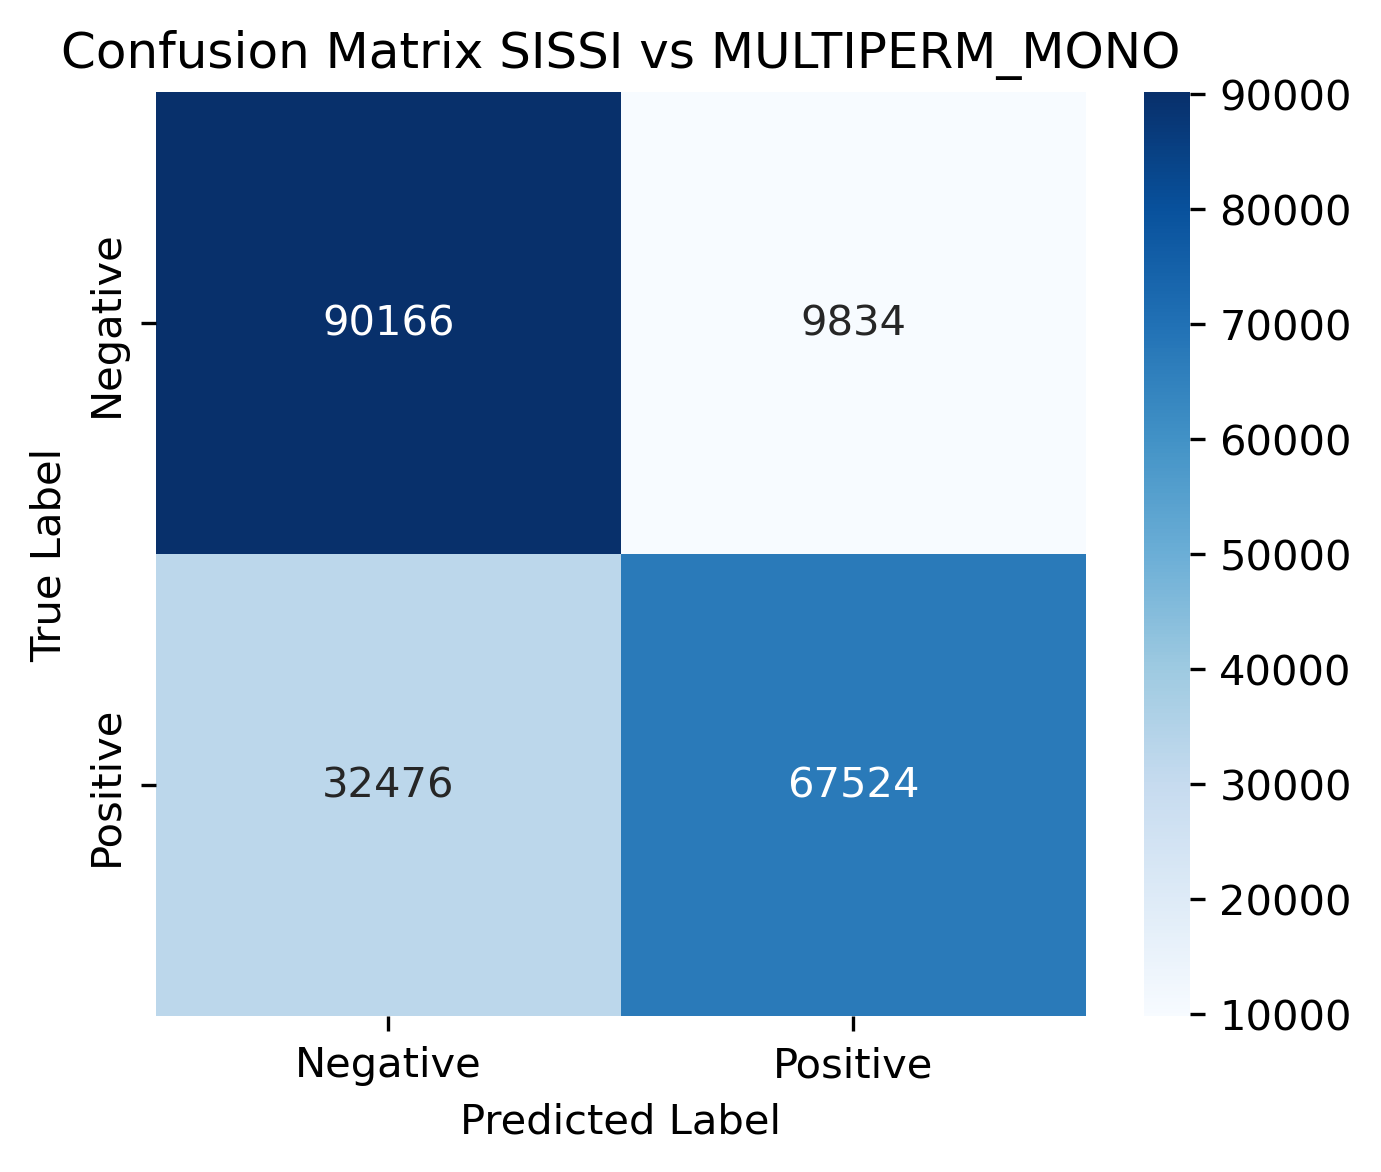
\includegraphics[width=\textwidth]{MXfold2_Confusion_Matrix_SISSI_vs_MULTIPERM_MONO.png}
        \caption{SISSI vs MULTIPERM-mono}
        \label{fig:confusion_multiperm_mono}
    \end{subfigure}
    \hfill
    \begin{subfigure}[b]{0.48\textwidth}
        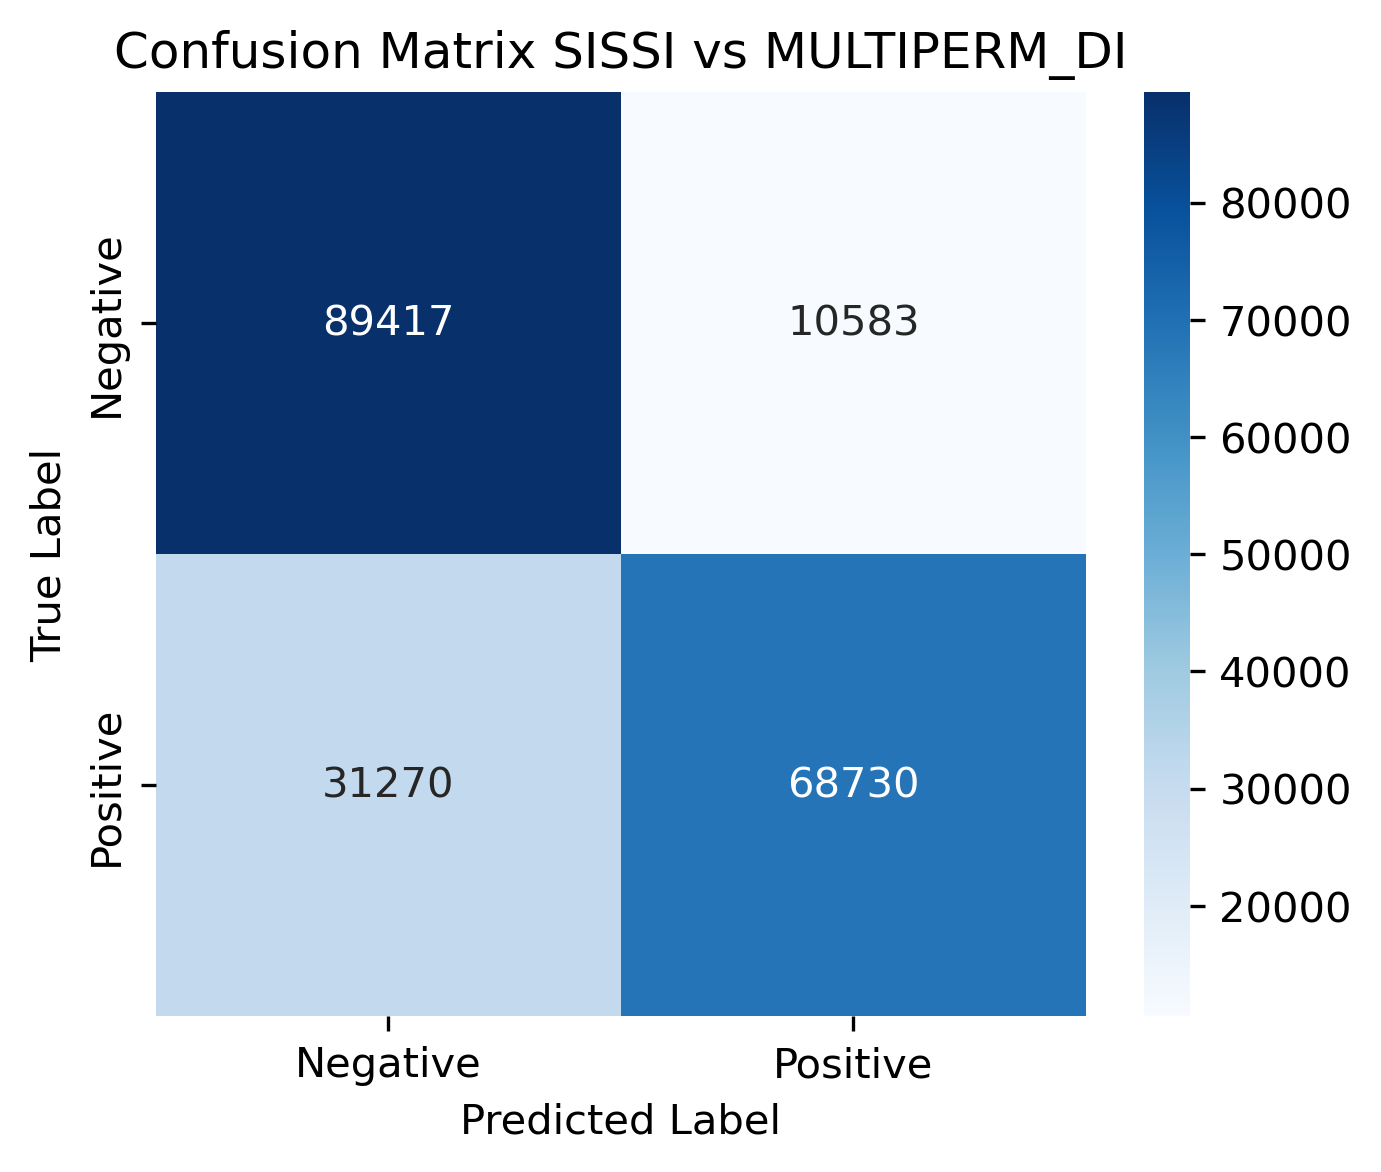
\includegraphics[width=\textwidth]{MXfold2_Confusion_Matrix_SISSI_vs_MULTIPERM_DI.png}
        \caption{SISSI vs MULTIPERM-di}
        \label{fig:confusion_multiperm_di}
    \end{subfigure}
    \vspace{1em}
    
    \begin{subfigure}[b]{0.48\textwidth}
        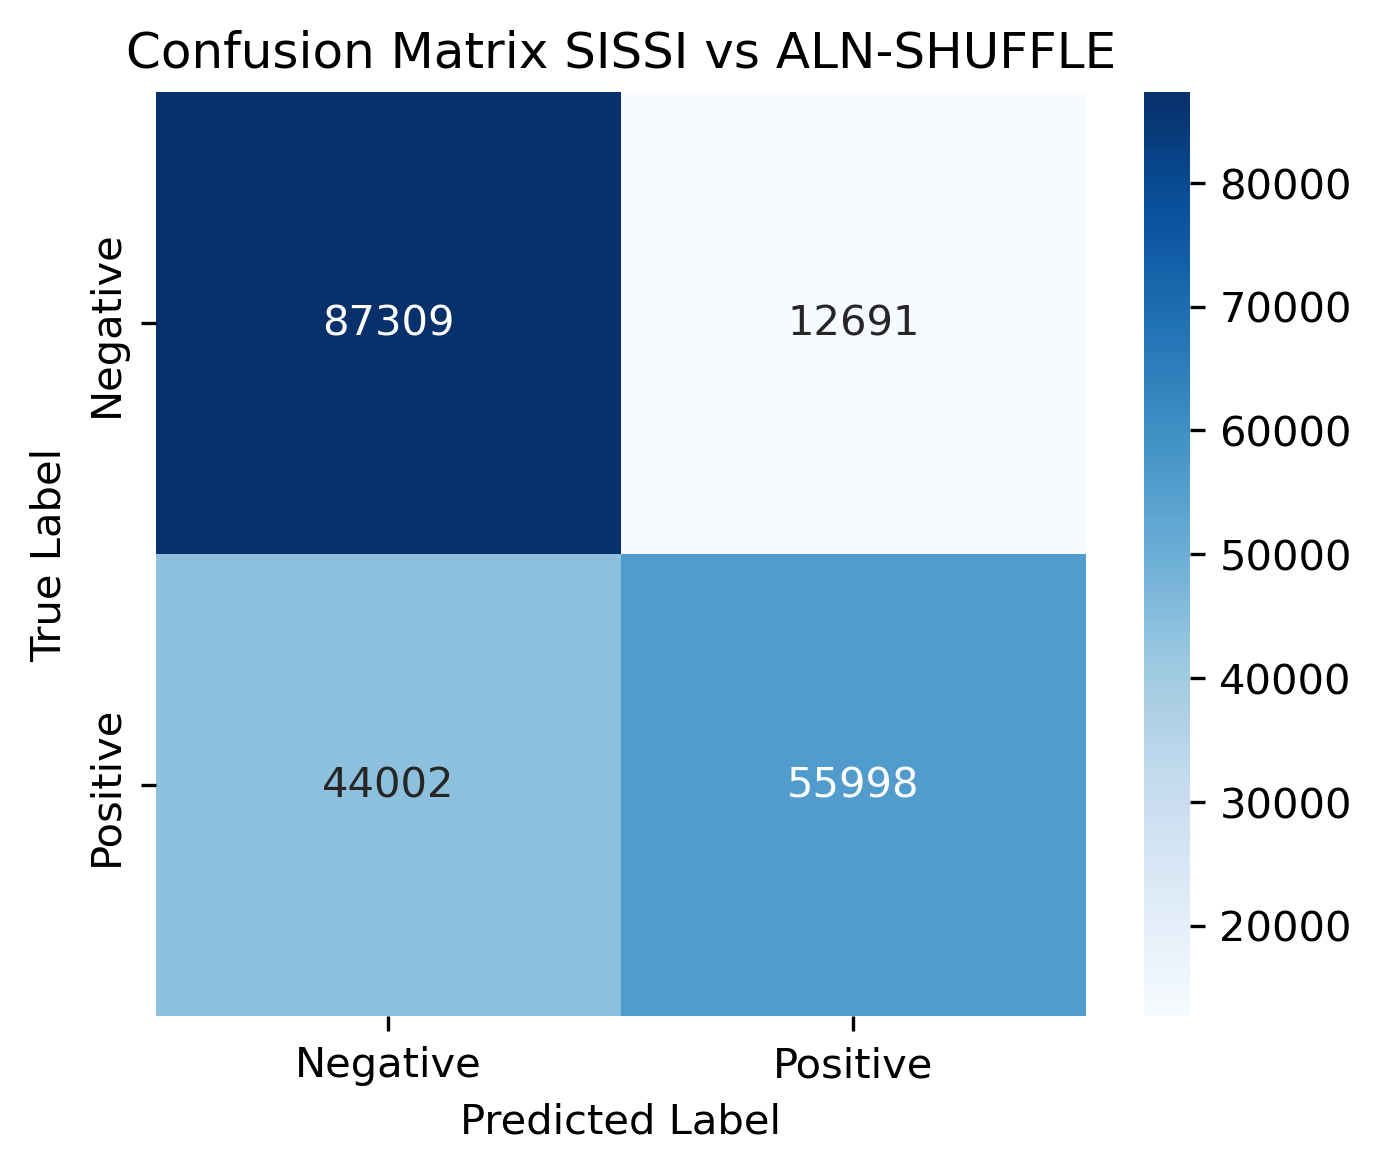
\includegraphics[width=\textwidth]{MXfold2_Confusion_Matrix_SISSI_vs_ALN-SHUFFLE.png}
        \caption{SISSI vs ALN-SHUFFLE}
        \label{fig:confusion_aln_shuffle}
    \end{subfigure}

    \caption{Confusion Matrix from MXfold2 prediction}
    \label{fig:all_confusionograms}
\end{figure}

The trends observed in the boxplot and histogram are further underpinned by the analysis of the confusion matrix. The separability of the models proves to be suboptimal. For the SISSIz-mono model (Figure a), 15,535 false-positive and 28,569 false-negative results were determined. The SISSIz-di model (Figure b) showed 17,546 false-positive and 34,018 false-negative results. \vspace{1em}    

The Multiperm-mono model (Figure c) yielded 9,834 false-positive and 32,476 false-negative results, while the Multiperm-di model (Figure d) performed similarly with 10,583 false-positive and 31,270 false-negative results. The Aln-shuffle model (Figure e) showed the worst results with 12,691 false-positive and 44,002 false-negative results.\vspace{1em}

\subsection{MXfold2 ROC-Kurven}

\begin{figure}[H]
    \centering
    \begin{subfigure}[b]{0.48\textwidth}
        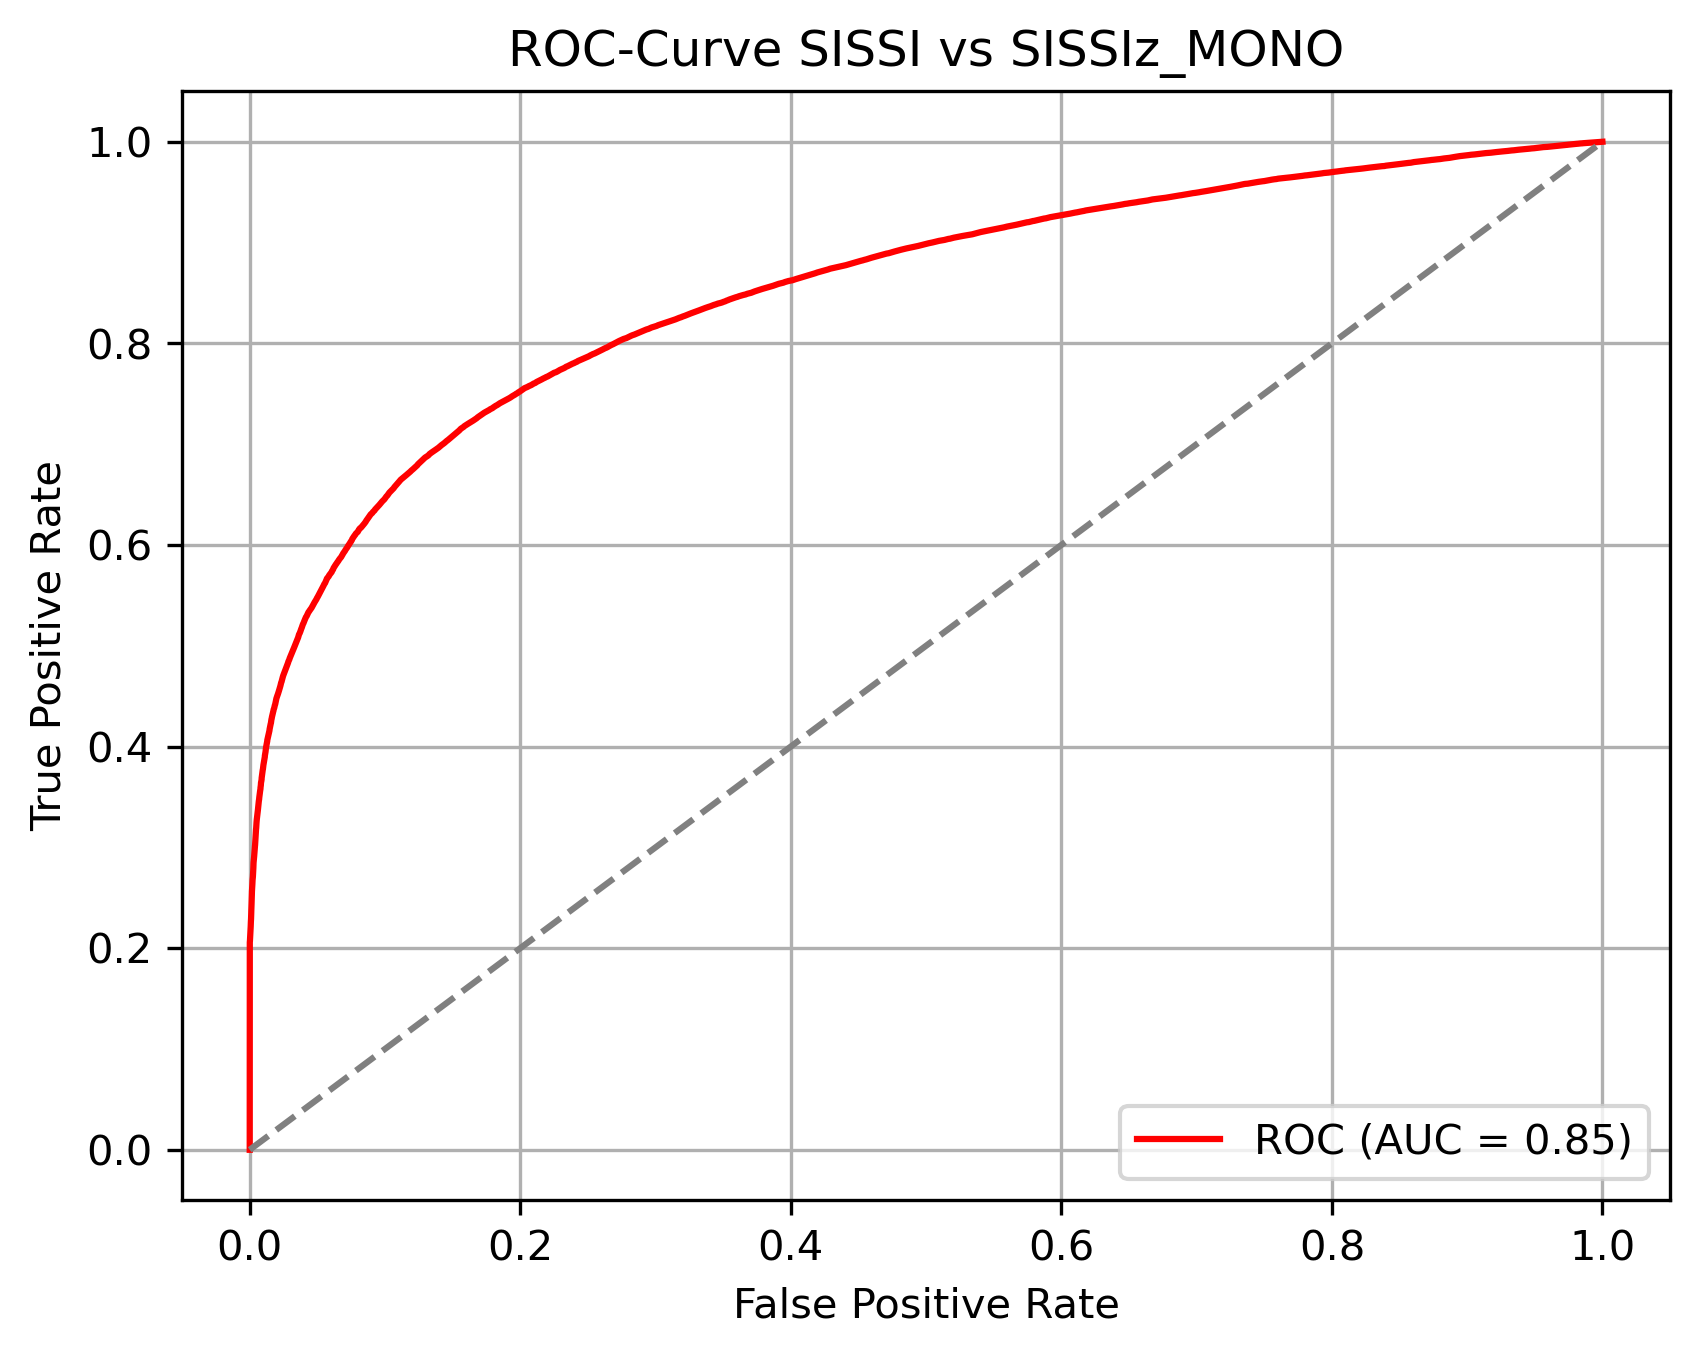
\includegraphics[width=\textwidth]{MXfold2_ROC_Curve_SISSI_vs_SISSIz_MONO.png}
        \caption{SISSI vs SISSIz-mono}
        \label{fig:roc_sissiz_mono}
    \end{subfigure}
    \hfill
    \begin{subfigure}[b]{0.48\textwidth}
        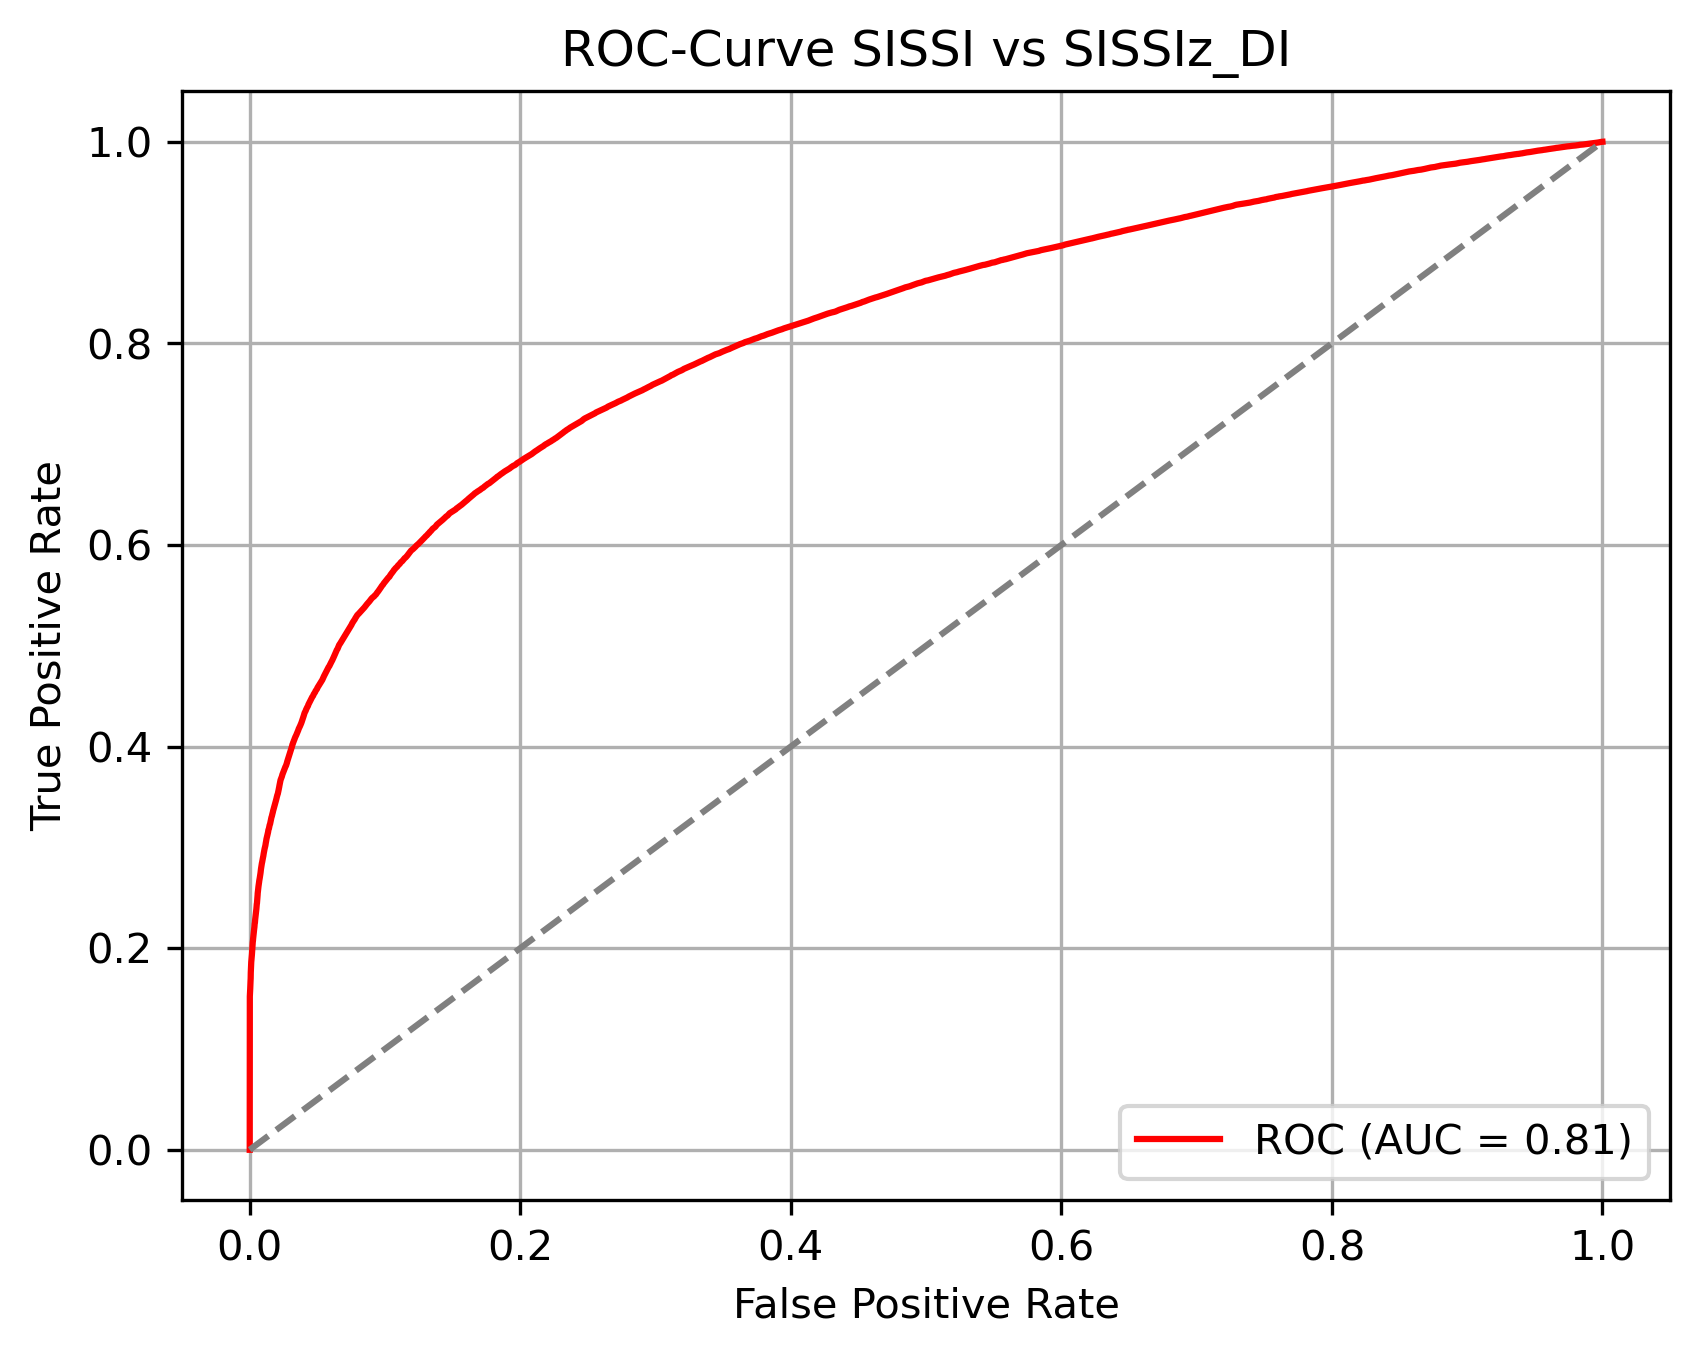
\includegraphics[width=\textwidth]{MXfold2_ROC_Curve_SISSI_vs_SISSIz_DI.png}
        \caption{SISSI vs SISSIz-di}
        \label{fig:roc_sissiz_di}
    \end{subfigure}
    \vspace{1em}

    \begin{subfigure}[b]{0.48\textwidth}
        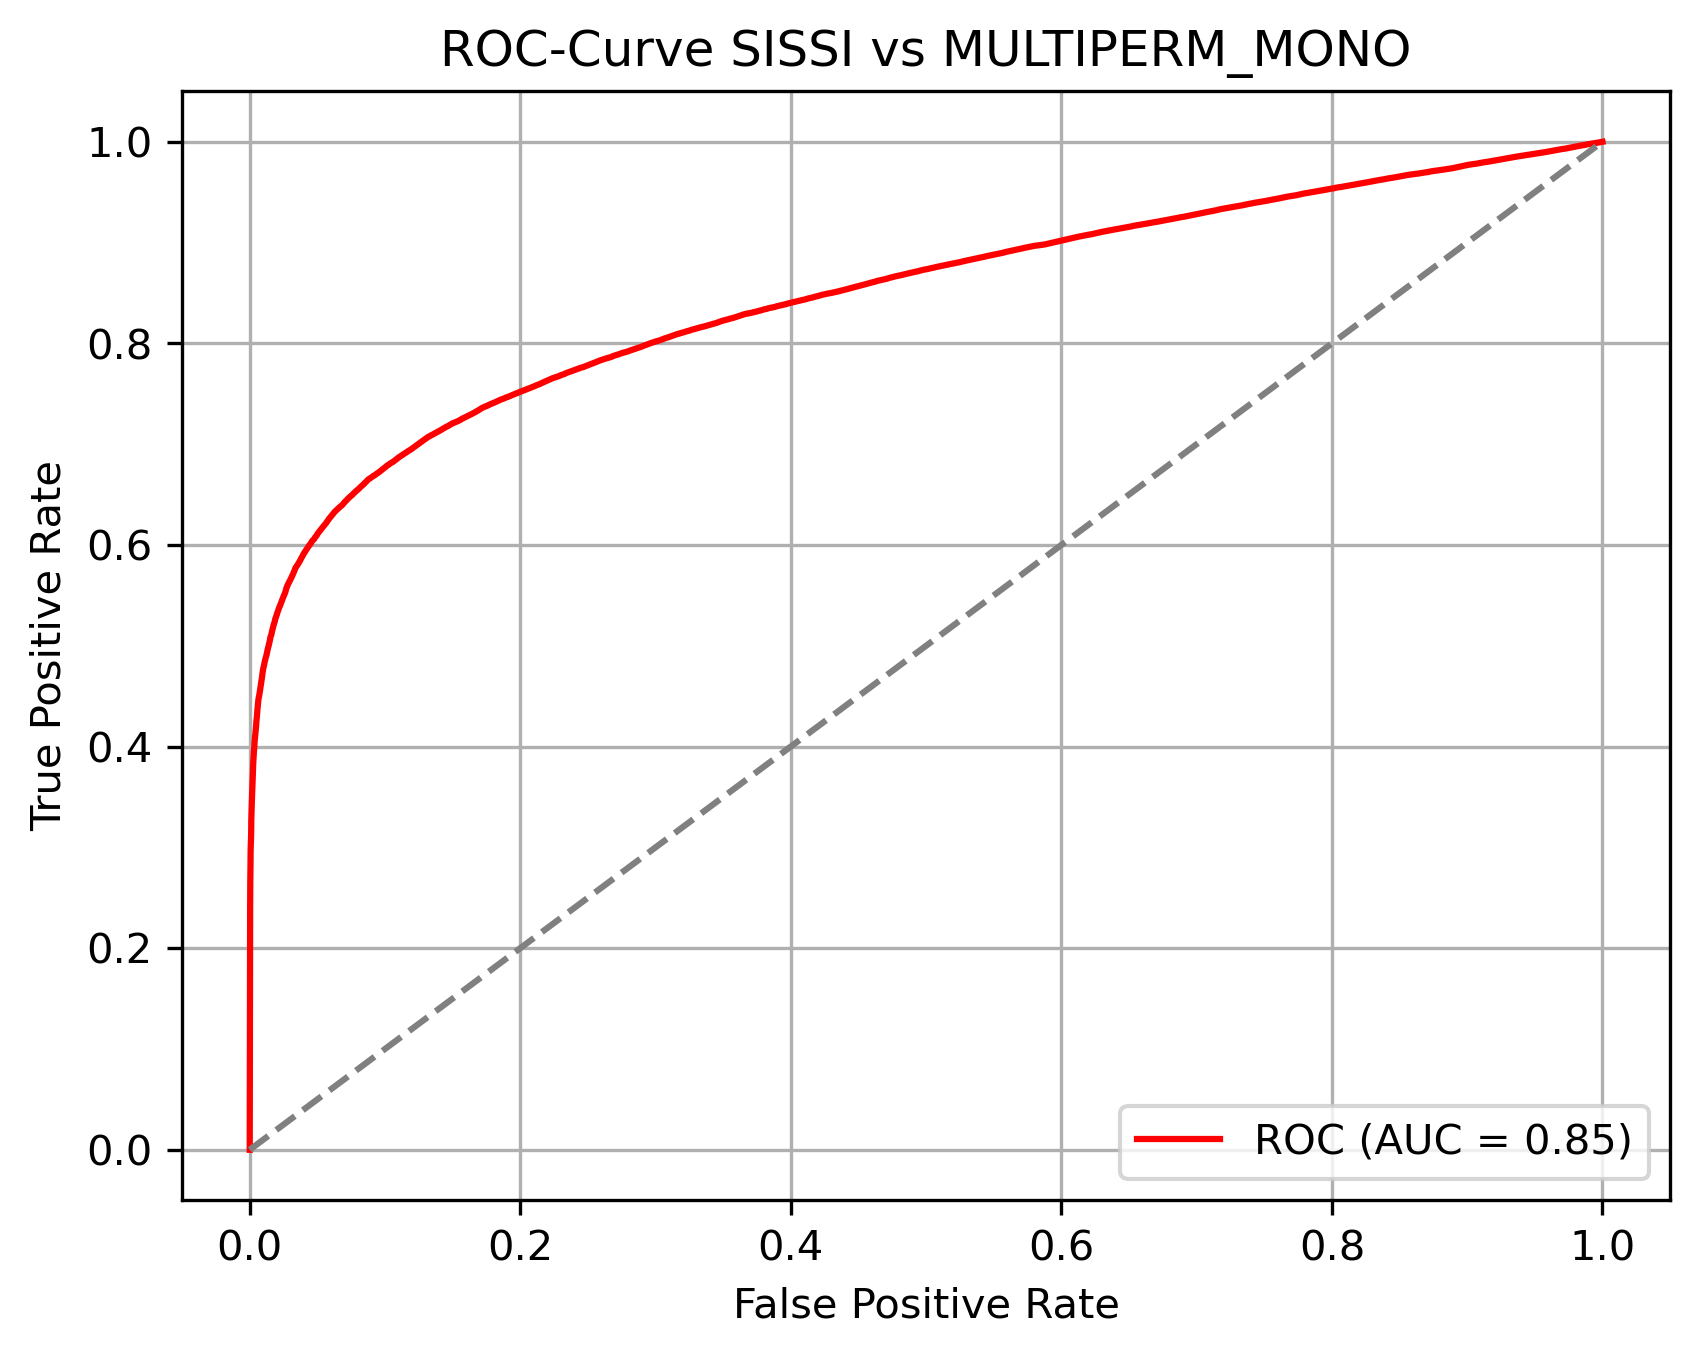
\includegraphics[width=\textwidth]{MXfold2_ROC_Curve_SISSI_vs_MULTIPERM_MONO.png}
        \caption{SISSI vs MULTIPERM-mono}
        \label{fig:roc_multiperm_mono}
    \end{subfigure}
    \hfill
    \begin{subfigure}[b]{0.48\textwidth}
        \includegraphics[width=\textwidth]{MXfold2_ROC_Curve_SISSI_vs_MULTIPERM_DI.png}
        \caption{SISSI vs MULTIPERM-di}
        \label{fig:roc_multiperm_di}
    \end{subfigure}
    \vspace{1em}

    \begin{subfigure}[b]{0.48\textwidth}
        \includegraphics[width=\textwidth]{MXfold2_ROC_Curve_SISSI_vs_ALN-SHUFFLE.png}
        \caption{SISSI vs ALN-SHUFFLE}
        \label{fig:roc_aln_shuffle}
    \end{subfigure}

    \caption{ROC-curves from MXfold2 prediction}
    \label{fig:all_roc_curves}
\end{figure}

The evaluation of the ROC curves for the MXfold2 models shows that none of the tested models provides satisfactory results. This could indicate that MXfold2 has difficulties in dealing with the simulated data generated by SISSI, leading to inaccurate prediction of RNA structural integrity.\vspace{1em}

Overall, the Multiperm-mono, Multiperm-di and SISSIz-mono model performs best, as they have a AUC score of 0.85, followed by SISSIz-di with 0.81. The last one is as excepted the Aln-shuffle with 0.77 \vspace{1em}

In view of these results, it would be of great interest to evaluate the models with real data in order to better assess their performance and applicability in practical scenarios. This could potentially lead to an improvement in the prediction accuracy and the general robustness of the models.

\clearpage

\section{Results of RNAz Prediction}

\subsection{RNAz Boxplot}

\begin{figure}[H]
    \centering
    \includegraphics[scale=0.7]{Boxplot RNAz SVM RNA-class probability.png}
    \caption{Boxplot MXfold2 Score}
    \label{fig:bar_chart}
\end{figure}

The boxplot illustrates the ability of different methods to destroy the RNA secondary structure. While the positive SISSI samples show very high RNAz probabilities as expected, the SISSIz-mono and SISSIz-di methods show significantly lower values and greater scatter. This indicates a successful destruction of the structure. In contrast, the RNAz values of the shuffling methods remain high, indicating insufficient structure destruction. Particularly striking is the Aln shuffling method, whose values are almost identical to the positive controls.

\subsection{RNAz Histograms}

\begin{figure}[H]
    \centering
    \begin{subfigure}[b]{0.48\textwidth}
        \includegraphics[width=\textwidth]{RNAz_Histogram_SISSI_vs_SISSIz_MONO.png}
        \caption{SISSI vs SISSIz-mono}
        \label{fig:hist_sissiz_mono}
    \end{subfigure}
    \hfill
    \begin{subfigure}[b]{0.48\textwidth}
        \includegraphics[width=\textwidth]{RNAz_Histogram_SISSI_vs_SISSIZ_DI.png}
        \caption{SISSI vs SISSIz-di}
        \label{fig:hist_sissiz_di}
    \end{subfigure}
    \vspace{1em}
    
    \begin{subfigure}[b]{0.48\textwidth}
        \includegraphics[width=\textwidth]{RNAz_Histogram_SISSI_vs_MULTIPERM_MONO.png}
        \caption{SISSI vs MULTIPERM-mono}
        \label{fig:hist_multiperm_mono}
    \end{subfigure}
    \hfill
    \begin{subfigure}[b]{0.48\textwidth}
        \includegraphics[width=\textwidth]{RNAz_Histogram_SISSI_vs_MULTIPERM_DI.png}
        \caption{SISSI vs MULTIPERM-di}
        \label{fig:hist_multiperm_di}
    \end{subfigure}
    \vspace{1em}
    
    \begin{subfigure}[b]{0.48\textwidth}
        \includegraphics[width=\textwidth]{RNAz_Histogram_SISSI_vs_ALN-SHUFFLE.png}
        \caption{SISSI vs ALN-SHUFFLE}
        \label{fig:hist_aln_shuffle}
    \end{subfigure}

    \caption{Histograms from RNAz prediction}
    \label{fig:all_histograms}
\end{figure}

The histograms also confirm the results of the boxplot analysis: the SISSIz-mono and SISSIz-di methods lead to a significant shift in the probability distribution towards low RNAz values, indicating effective destruction of the RNA secondary structure. In contrast, the shuffling methods show hardly any change in the distribution compared to the positive control, indicating insufficient impairment of the structure.

\subsection{RNAz Confusion Matrix}

\begin{figure}[H]
    \centering
    \begin{subfigure}[b]{0.48\textwidth}
        \includegraphics[width=\textwidth]{RNAz_Confusion_Matrix_SISSI_vs_SISSIz_MONO.png}
        \caption{SISSI vs SISSIz-mono}
        \label{fig:confusion_sissiz_mono}
    \end{subfigure}
    \hfill
    \begin{subfigure}[b]{0.48\textwidth}
        \includegraphics[width=\textwidth]{RNAz_Confusion_Matrix_SISSI_vs_SISSIZ_DI.png}
        \caption{SISSI vs SISSIz-di}
        \label{fig:confusion_sissiz_di}
    \end{subfigure}
    \vspace{1em}
    
    \begin{subfigure}[b]{0.48\textwidth}
        \includegraphics[width=\textwidth]{RNAz_Confusion_Matrix_SISSI_vs_MULTIPERM_MONO.png}
        \caption{SISSI vs MULTIPERM-mono}
        \label{fig:confusion_multiperm_mono}
    \end{subfigure}
    \hfill
    \begin{subfigure}[b]{0.48\textwidth}
        \includegraphics[width=\textwidth]{RNAz_Confusion_Matrix_SISSI_vs_MULTIPERM_DI.png}
        \caption{SISSI vs MULTIPERM-di}
        \label{fig:confusion_multiperm_di}
    \end{subfigure}
    \vspace{1em}
    
    \begin{subfigure}[b]{0.48\textwidth}
        \includegraphics[width=\textwidth]{RNAz_Confusion_Matrix_SISSI_vs_ALN-SHUFFLE.png}
        \caption{SISSI vs ALN-SHUFFLE}
        \label{fig:confusion_aln_shuffle}
    \end{subfigure}

    \caption{Confusion Matrix from RNAz prediction}
    \label{fig:all_confusionograms}
\end{figure}

An interesting result can be seen when analyzing the confusion matrices: The shuffle methods have lower overall values for false-positive (FP) and false-negative (FN) classifications. The best values are achieved by Multiperm-di with 70 FP and 717 FN, followed by Multiperm-mono with 83 FP and 706 FN. ALN-shuffle also achieves lower error rates than the SISSIz-based methods with 144 FP and 2052 FN.\vspace{1em}

However, these seemingly positive values should be viewed critically. The reason for the low FP and FN values for the shuffle methods lies in the low discriminatory power of the classification: The p-values of the negative controls are very close to those of the positive sample (SISSI), so that the model can hardly distinguish between the classes.\vspace{1em}

In contrast, SISSIz-mono (2262 FP, 6885 FN) and SISSIz-di (3262 FP, 8145 FN) show a significantly higher misclassification rate. However, this results from an overall better separability.\vspace{1em}

In summary, it can be said that the SISSIz-mono and SISSIz-di methods cause a more effective destruction of the RNA secondary structure and thus enable an improved classification. Despite higher misclassifications numbers, they provide the most convincing results overall in terms of discriminatory power and classification performance.\vspace{1em}

\subsection{RNAz ROC-Kurven}

\begin{figure}[H]
    \centering
    \begin{subfigure}[b]{0.48\textwidth}
        \includegraphics[width=\textwidth]{RNAz_ROC_Curve_SISSI_vs_SISSIz_MONO.png}
        \caption{SISSI vs SISSIz-mono}
        \label{fig:roc_sissiz_mono}
    \end{subfigure}
    \hfill
    \begin{subfigure}[b]{0.48\textwidth}
        \includegraphics[width=\textwidth]{RNAz_ROC_Curve_SISSI_vs_SISSIZ_DI.png}
        \caption{SISSI vs SISSIz-di}
        \label{fig:roc_sissiz_di}
    \end{subfigure}
    \vspace{1em}

    \begin{subfigure}[b]{0.48\textwidth}
        \includegraphics[width=\textwidth]{RNAz_ROC_Curve_SISSI_vs_MULTIPERM_MONO.png}
        \caption{SISSI vs MULTIPERM-mono}
        \label{fig:roc_multiperm_mono}
    \end{subfigure}
    \hfill
    \begin{subfigure}[b]{0.48\textwidth}
        \includegraphics[width=\textwidth]{RNAz_ROC_Curve_SISSI_vs_MULTIPERM_DI.png}
        \caption{SISSI vs MULTIPERM-di}
        \label{fig:roc_multiperm_di}
    \end{subfigure}
    \vspace{1em}

    \begin{subfigure}[b]{0.48\textwidth}
        \includegraphics[width=\textwidth]{RNAz_ROC_Curve_SISSI_vs_ALN-SHUFFLE.png}
        \caption{SISSI vs ALN-SHUFFLE}
        \label{fig:roc_aln_shuffle}
    \end{subfigure}

    \caption{ROC-curves from RNAz prediction}
    \label{fig:all_roc_curves}
\end{figure}

The highest AUC values of 1.00 were achieved with the shuffle-based control methods (Multiperm-mono, Multiperm-di and ALN-shuffle). These values indicate an almost perfect differentiation of the classes in terms of score ranking.\vspace{1em}

However, this seemingly ideal classification must be viewed in a differentiated manner. Although a high AUC value means that positive instances tend to receive higher scores than negative ones, it says nothing about the absolute separability at a specific threshold value. The shuffle methods in particular show that, despite high AUC values, the actual class separation is less pronounced, which is reflected in the relatively low p-value differences between positive and negative examples.\vspace{1em}

In contrast, the SISSIz-mono and SISSIz-di models have slightly lower values with AUC values of 0.98, but show a clearer separation of the classes along the score spectrum. This stronger separation leads to improved classification performance in practical application, especially with fixed decision limits. This is demonstrated, among other things, by the clearly different score distributions and the results of the confusion matrices.\vspace{1em}

In summary, it can be stated that the AUC values of all models indicate a fundamentally high classification quality. However, despite slightly lower AUC values, the SISSIz-mono and SISSIz-di methods offer a more robust separation of classes that is easier to use in practice, making them particularly effective negative control methods in the given classification context.\vspace{1em}

\clearpage

\section{SPOT-RNA2}

For the prediction of RNA secondary structures, I downloaded the NCBI database \texttt{nt-prok.\*.tar.gz} (26 compressed files in total). This should be sufficient to ensure broad coverage of prokaryotic sequences.\vspace{1em}

An initial problem was that SPOT-RNA2 did not recognize the database correctly. This could be fixed by creating a dummy file named \texttt{nt-prok} and adjusting the paths accordingly.\vspace{1em}

The script \texttt{run\_spotrna2.sh} can be executed successfully. However, the runtime per file is around 3909 seconds. For a total data volume of 600,000 sequences, processing would theoretically take around 74 years.\vspace{1em}

The biggest bottleneck is the use of the \texttt{Infernal} tool, which can only be executed on the CPU. As the server used only has 48 CPU cores and these are fully utilized, it is not possible to parallelize the process.\vspace{1em}

\textbf{Possible solution approaches:}\vspace{1em}
\begin{itemize}
    \item[\textbf{(1)}] Skipping the \texttt{Infernal} step, but this can lead to a lower prediction accuracy.
    \item[\textbf{(2)}] Use of a smaller database, which could also negatively affect the prediction quality
\end{itemize}

If no solution is found for SPOT-RNA2 then I will look around for alternatives. (e.g.: UFold, E2EFold,...)

\section{References}
\begin{itemize}
    \item[\textbf{[1]}] \url{https://doi.org/10.1038/s41467-021-21194-4    } \par
    \item[\textbf{[2]}] \url{https://github.com/mxfold/mxfold2?tab=readme-ov-file} \par
\end{itemize}

\end{large}
\end{document}

Summary KW23 - KW24

\documentclass{article}
\usepackage{graphicx} % Required for inserting images
\usepackage{hyperref}
\usepackage{setspace}
\usepackage{listings}
\usepackage{float}
\usepackage[font=small,labelfont=bf]{caption}
\usepackage[a4paper, margin=1in]{geometry}
\usepackage{setspace}  
\onehalfspacing
\usepackage{hyperref}
\usepackage{xcolor}
\usepackage{graphicx}
\usepackage{caption}
\usepackage{subcaption}
\hypersetup{
    colorlinks=true, 
    linkcolor=blue, 
    urlcolor=blue,  
}

\usepackage{listings}
\usepackage{xcolor}

\lstset{
    language=Python,
    basicstyle=\ttfamily\small,
    keywordstyle=\bfseries\color{blue},
    commentstyle=\itshape\color{gray},
    stringstyle=\color{orange},
    showstringspaces=false,
    numbers=left,
    numberstyle=\tiny,
    breaklines=true,
    frame=single
    aboveskip=1em,
    belowskip=1em
}


% Einstellungen für Code Listings
\lstset{
basicstyle=\ttfamily\small,
breaklines=true,
frame=single
}

\setlength{\parindent}{0pt}
\setlength{\textfloatsep}{0pt}

\title{KW23 - KW24 Summary}
\author{Stefan Redl}
\begin{document}
\maketitle

\begin{large}

\section{Methods that i try to used}

\subsection{{SPOT-RNA}\href{https://doi.org/10.1038/s41467-019-13395-9 }{\textbf{[1]}}\href{https://github.com/jaswindersingh2/SPOT-RNA}{\textbf{[2]}}}

The installation of SPOT-RNA went smoothly and the initial results also looked promising. Unfortunately, the tool required around three days to predict 3000 samples when the available resources were fully utilized. Extrapolated to 600,000 samples, this would lead to an impractically long runtime. The use of SPOT-RNA was therefore discontinued and the focus shifted to alternative tools.

\subsection{{SPOT-RNA2}\href{https://doi.org/10.1093/bioinformatics/btab165}{\textbf{[3]}}\href{https://github.com/jaswindersingh2/SPOT-RNA2}{\textbf{[4]}}}

SPOT-RNA2 also showed a very long prediction runtime. The computing time required per sample remained high despite the reduction in data volume, as SPOT-RNA and Infernal are very time-consuming. A significant acceleration could not be achieved.

\subsection{{UFold}\href{https://doi.org/10.1093/nar/gkab1074}{\textbf{[5]}}\href{https://github.com/uci-cbcl/UFold}{\textbf{[6]}}}

UFold was tested next. First issue was that the source code has some conflicts. After i solved the problems UFold could be used for the prediction. This tool does not support MSA files, only single-sequence fasta files. An attempt was therefore made to split the MSA files into individual sequences and generate suitable input files from them. This worked well and UFold provided fast predictions. One disadvantage, however, was that no real parallelization was possible, since UFold only ever works with a fixed input file (`input.txt`). Attempts to run multiple instances simultaneously failed. In addition, the output in dot-bracket notation was sometimes incorrect: brackets were missing or there were too many, which meant that no valid MFE calculation with RNAeval was possible.

\subsection{{E2Efold}\href{https://doi.org/10.48550/arXiv.2002.05810}{\textbf{[7]}}\href{https://github.com/ml4bio/e2efold}{\textbf{[8]}}}

E2Efold follows a similar concept to UFold and is also its predecessor version. As it is no longer actively maintained, a functioning installation on the server was not possible.

\subsection{{AliNA}\href{https://doi.org/10.1002/minf.202300113}{\textbf{[9]}}\href{https://github.com/Arty40m/AliNA}{\textbf{[10]}}}

AliNA is a relatively new tool for the prediction of RNA secondary structures. Installation and execution were straightforward, and the support of MSA data was a big advantage - no splitting of sequences was required. Unfortunately, AliNA only supports alignments up to a maximum length of 256 nucleotides. My alignment had a length of 401, and adjusting this limit in the code did not make sense as the model was only trained on sequences up to 256. An extension would have led to poor predictions. Without this limitation, AliNA would have been a suitable solution.

\subsection{{sincFold}\href{https://doi.org/10.1093/bib/bbae271}{\textbf{[11]}}\href{https://github.com/sinc-lab/sincFold}{\textbf{[12]}}}

The installation and setup of sincFold also went smoothly. However, the tool delivered strange results when processing my MSA fasta files: Only one sequence was ever predicted - seemingly selected at random. The tool is therefore not suitable for MSA data. In addition, the prediction time was relatively long.

\subsection{{REDFold}\href{https://doi.org/10.1186/s12859-023-05238-8}{\textbf{[13]}}\href{https://github.com/aky3100/REDfold}{\textbf{[14]}}}

Finally, REDFold was tested. Although it only accepts single sequences as input, its speed and GPU support were convincing. The installation went smoothly and the results in dot-bracket notation were formally correct. Based on these positive aspects, a full test run was started. The computing time for 234,000 fasta sequences was around 10 hours with sequential GPU use. Parallelization of the GPU processes could enable further optimizations here. However, it turned out that REDFold temporarily requires a lot of RAM - of the available 187.5 GB RAM, up to 141.5 GB was used at times. The content analysis of the results is still pending, but is being planned.

\section{References}
\begin{itemize}
    \item[\textbf{[1]}] \url{https://doi.org/10.1038/s41467-019-13395-9} \par
    \item[\textbf{[2]}] \url{https://github.com/jaswindersingh2/SPOT-RNA} \par
    
    \item[\textbf{[3]}] \url{https://doi.org/10.1093/bioinformatics/btab165} \par
    \item[\textbf{[4]}] \url{https://github.com/jaswindersingh2/SPOT-RNA2} \par
    
    \item[\textbf{[5]}] \url{https://doi.org/10.1093/nar/gkab1074} \par
    \item[\textbf{[6]}] \url{https://github.com/uci-cbcl/UFold} \par
    
    \item[\textbf{[7]}] \url{https://doi.org/10.48550/arXiv.2002.05810} \par
    \item[\textbf{[8]}] \url{https://github.com/ml4bio/e2efold} \par
    
    \item[\textbf{[9]}] \url{https://doi.org/10.1002/minf.202300113} \par
    \item[\textbf{[10]}] \url{https://github.com/Arty40m/AliNA} \par
    
    \item[\textbf{[11]}] \url{https://doi.org/10.1093/bib/bbae271} \par
    \item[\textbf{[12]}] \url{https://github.com/sinc-lab/sincFold} \par
    
    \item[\textbf{[13]}] \url{https://doi.org/10.1186/s12859-023-05238-8} \par
    \item[\textbf{[14]}] \url{https://github.com/aky3100/REDfold} \par
\end{itemize}

\end{large}
\end{document}



